\documentclass{beamer}
\usepackage[utf8]{inputenc}
\usepackage{hyperref}
\usepackage{colortbl}
\usepackage{epstopdf}
\usepackage{graphicx}
\usepackage{mathtools}
\usepackage{listings}
\usepackage{letltxmacro}
\usepackage[noend]{algorithm, algpseudocode}

\usepackage{amsmath}
\usepackage{amssymb}

\usepackage{pgfplots}

\usepackage{mathtools}
\newcommand\myeq{\stackrel{\mathclap{\normalfont\mbox{def}}}{=}}

\newcommand{\idest}{{\it i.e.}}
\newcommand{\exemp}{{\it e.g.}}
\newcommand{\etc}{{\it etc.}}
\newcommand{\etal}{{\it et al.}}

\lstdefinelanguage
{PDDL}[]{LISP}
{alsoletter={:,?}, 
morekeywords={define,domain,problem,:domain,:extends,:requirements,:strips,:equality,:typing,:conditional-effects,:strips,:types,:objects,:negative-preconditions,:disjunctive-preconditions,:existential-preconditions,:universal-preconditions, :constants,:domain-variables,:timeless,:domain-axioms,:action-expansions,:predicates,:action,:parameters,:precondition,:effect,:fluents,:primary-effect,:side-effect,:init,:goal,when,not,forall,exists,goal-type,choice,forsome,in-context}}
%[[⟨list of required aspects (keywordcomments,texcs,etc.)⟩]]

\lstdefinelanguage
{SHOP}[]{LISP}
{alsoletter={:,?,!}, 
morekeywords={defdomain,defproblem,:domain,:method,:operator
:goal,when,not,forall,exists,goal-type,choice,forsome,in-context}}


\lstset{language=PDDL}

\newcommand{\todo}[1]{ {\color{red} #1} }

\def\masterclass{1}
% \def\masterclass{0}

\usetheme{Madrid}
\usecolortheme{seagull}
\title[\fontsize{0.08cm}{1em}\selectfont Plan and Goal Recognition]{Plan and Goal Recognition \\ SICSA DVF Master Class}
\author[Meneguzzi]{Felipe Meneguzzi\dag
}
\institute[]{\dag Pontifical Catholic University of Rio Grande do Sul, Brazil
\\
\url{felipe.meneguzzi@pucrs.br}
}
\date{Aberdeen, October, 2017}

\setbeamertemplate{subsection page}
{
    \begingroup
    \begin{beamercolorbox}[sep=12pt,center]{section title}
        \usebeamerfont{section title}\insertsection\par
    \end{beamercolorbox}
    \vspace*{10pt}
    \begin{beamercolorbox}[sep=8pt,center]{subsection title}
        \usebeamerfont{subsection title}\insertsubsection\par
    \end{beamercolorbox}
    \endgroup
}

\AtBeginSection[]
{
  \begin{frame}
    \frametitle{Table of Contents}
    \tableofcontents[currentsection]
  \end{frame}
}

\AtBeginSubsection[]
{
  \frame{\subsectionpage}
}

\begin{document}

%---------------------------------------------------------------------------------

    \begin{frame}
        \titlepage
    \end{frame}
    
%---------------------------------------------------------------------------------
\section{Introduction}

\subsection[Test]{Motivation and Intuition}
	% \begin{frame}[c]\frametitle{Tentative Structure}
% 		\begin{itemize}
% 			\item Introduction to plan recognition (from Automated Planning)
% 			\item Goal recognition heuristics
% 			\item Hybrid goal recognition heuristics (ask Mor)
% 			\item Optimality monitoring and applications
% 			\item Recognizing plans using real-time video data
% 			\item Future work
% 		\end{itemize}
% 	\end{frame}

	\begin{frame}[c]\frametitle{Overview}
		\begin{itemize}
			\item Recognizing plans and goals of others is a critical ability for intelligent interaction:
			\begin{itemize}
				\item important for humans/agents working in the same environment
				\item increasingly important as we build more intelligent systems
			\end{itemize}
			\item Overall area of Plan, Activity and Intent Recognition
			\begin{itemize}
				\item Activity recognition: recognizing meaningful activities from low-level sensor data
				\item Plan/Intent/Goal recognition: recognizing intentional higher-level sequences of activities 
			\end{itemize}
		\end{itemize}
	\end{frame}

	\begin{frame}[c]\frametitle{Goal Recognition}
		\begin{itemize}
			\item \textbf{Goal Recognition} is the task of recognizing agents' goal that explains a sequence of observations of its actions;
			\begin{itemize}
				\item Related to plan recognition, i.e. recognizing a \emph{top-level} action
				\item A specific form of the problem of abduction 
			\end{itemize}
			\item Approaches to goal and plan recognition divided into roughly two types:
			\begin{itemize}
				\item Plan-library based (\emph{classical} plan recognition)
				\item Domain-theory based (plan recognition as planning, or PRAP)
			\end{itemize}
		\end{itemize}
	\end{frame}
	
	\begin{frame}[c]\frametitle{Flavors of Recognition Formalism}
		\begin{columns}
			\begin{column}[t]{0.5\textwidth}
				Plan Library
				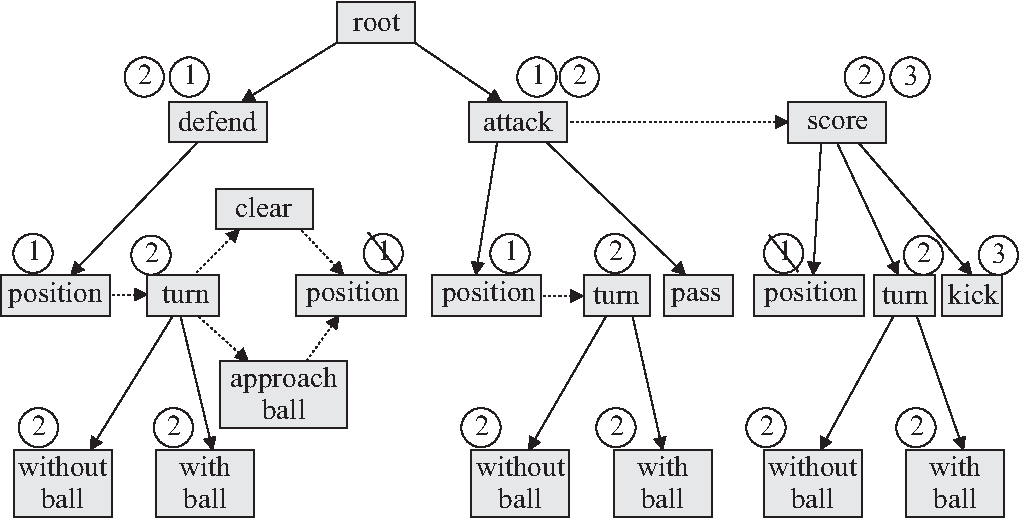
\includegraphics[width=\textwidth]{examples/fig_plan_library.pdf}
			\end{column}
			\begin{column}[t]{0.5\textwidth}
				Domain Theory (PRAP)
				\lstinputlisting[basicstyle=\fontsize{4}{4.5}\selectfont,language=PDDL]{examples/easy_ipc_grid.pddl.txt}
			\end{column}
		\end{columns}
	\end{frame}
	
	\begin{frame}[c]\frametitle{An example of Activity Recognition}
		% \animategraphics[loop,type=png,width=\linewidth]{2}{fig/egg-}{1}{4}
		\begin{center}
			\only<1>{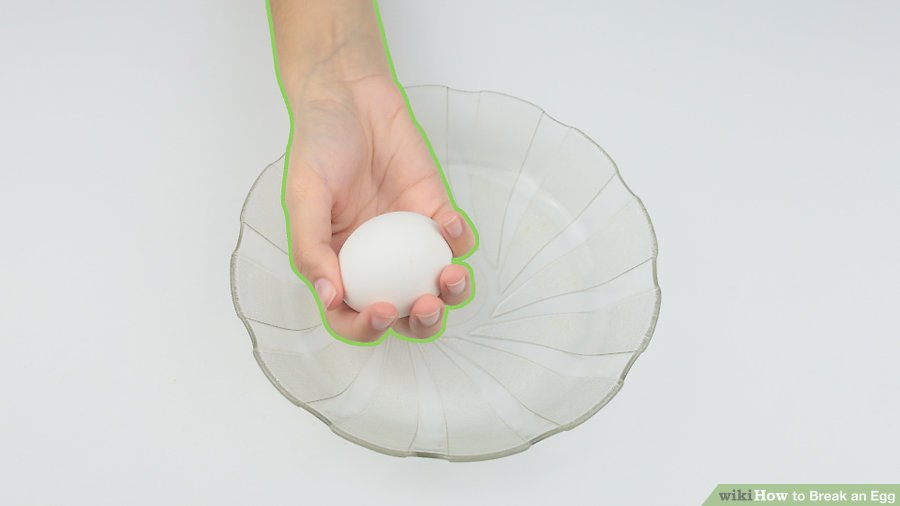
\includegraphics[width=.5\linewidth]{fig/egg-1.jpg}}
			\only<2>{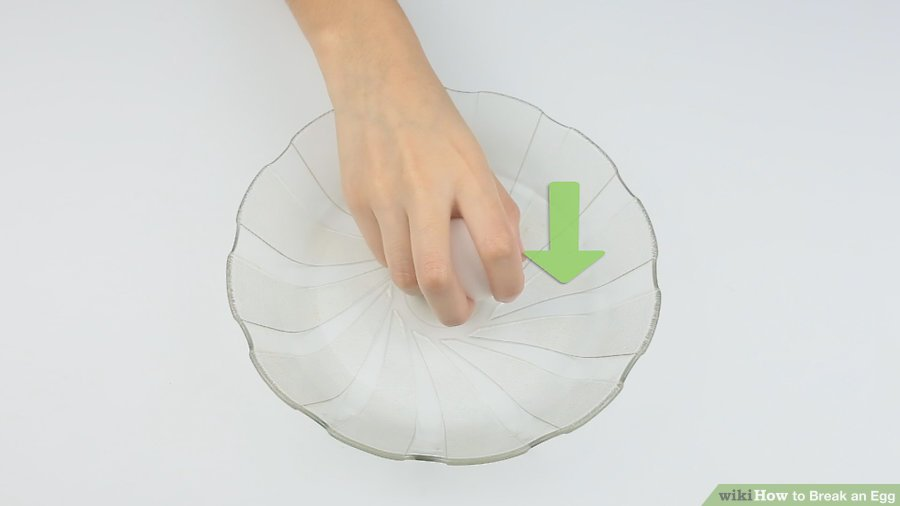
\includegraphics[width=.5\linewidth]{fig/egg-2.jpg}}
			\only<3>{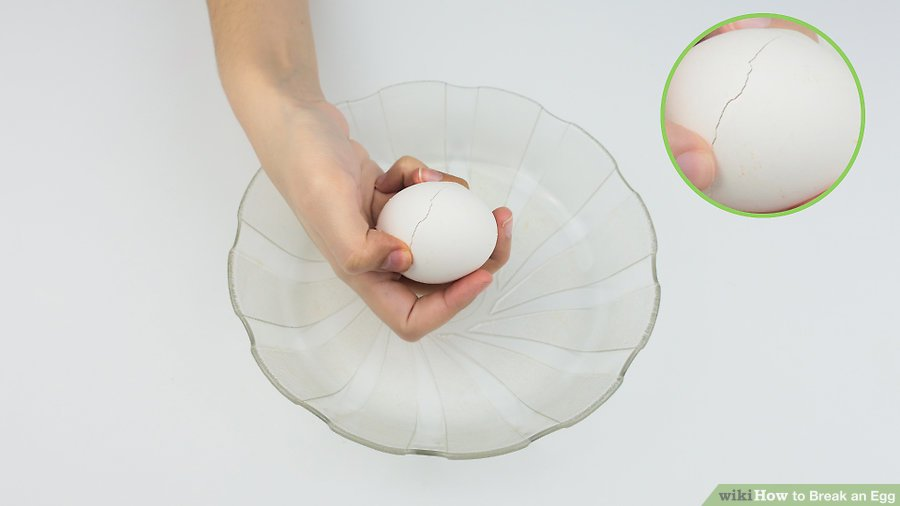
\includegraphics[width=.5\linewidth]{fig/egg-3.jpg}}
			\only<4>{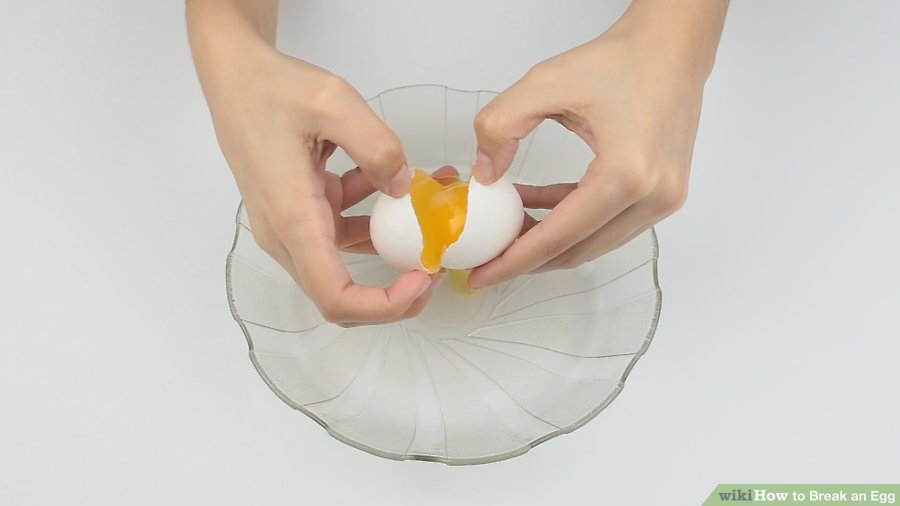
\includegraphics[width=.5\linewidth]{fig/egg-4.jpg} \\
			\texttt{breaking egg}
			}
		\end{center}
		% {\color{red} Complete this once I figure out how to include graphics}
		
	\end{frame}
	
	\begin{frame}[c]\frametitle{An Example of Goal/Plan Recognition}
		from Miquel Ramirez's thesis
		\begin{columns}
			\begin{column}{0.5\textwidth}
			    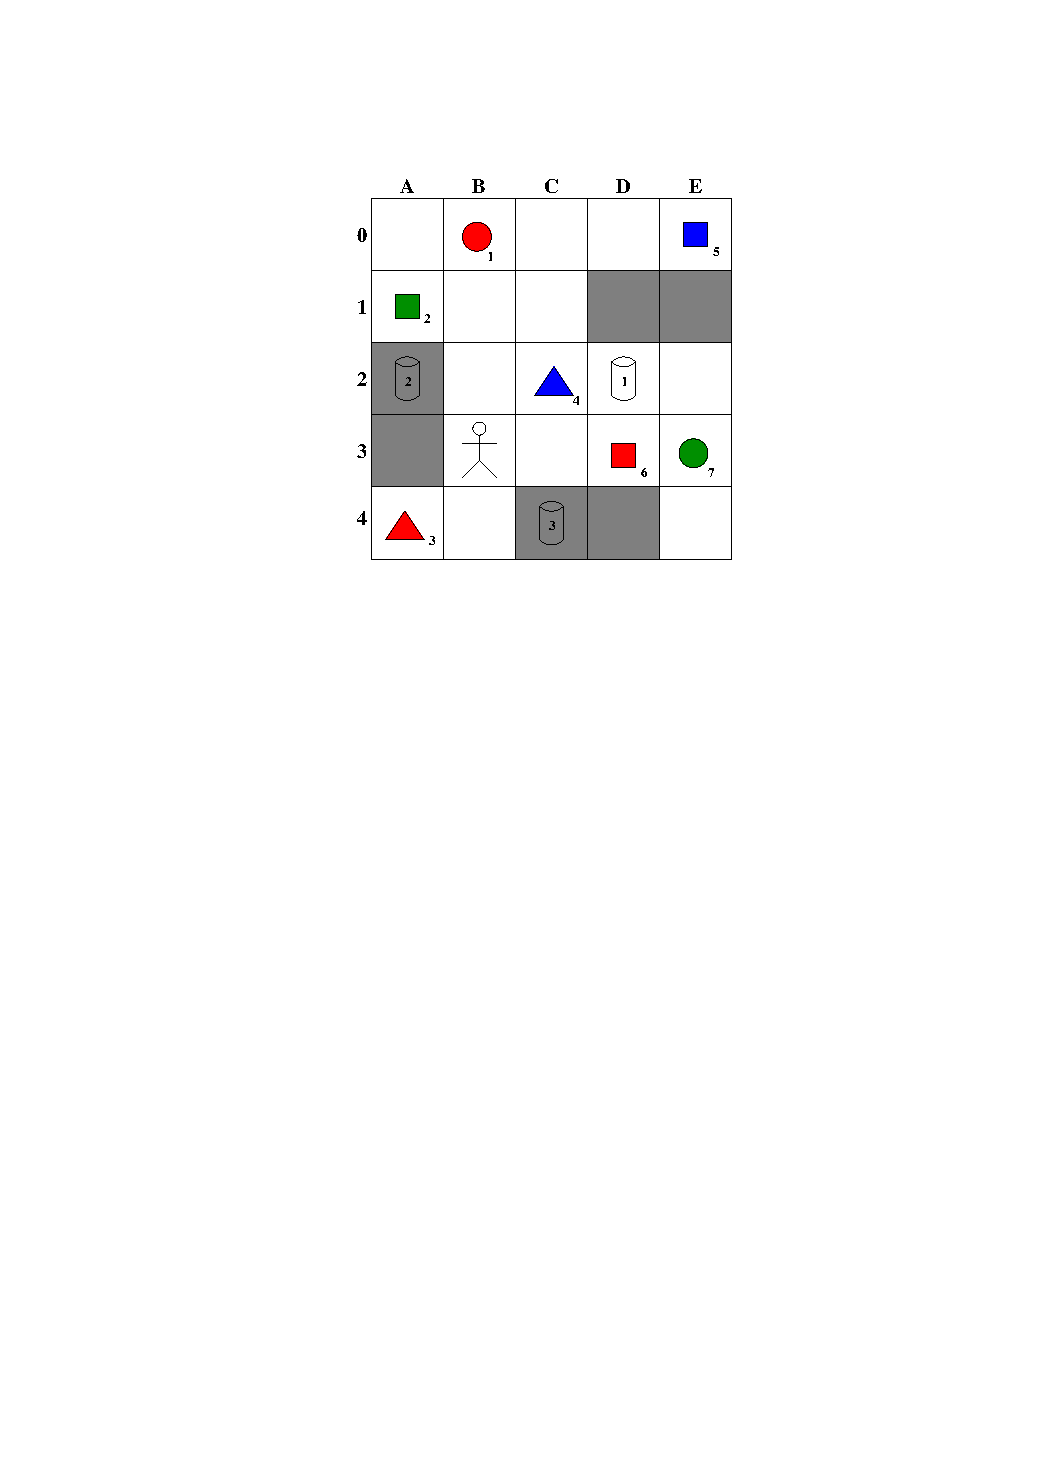
\includegraphics[width=.9\textwidth]{fig/roboschool-example.pdf}\\
				Wooden pieces $p_1,p_2, \dots p_n$\\
				Pieces have shapes and colors\\
				Bins $b_1, b_2, \dots, b_n$
			\end{column}
			\begin{column}{0.5\textwidth}
			\only<1>{
			The possible \textbf{goals} the trainer expected to pursue:
			\begin{enumerate}
				\item Store all triangles in $b_1$
				\item Store all spheres in $b_2$
				\item Store all cubes in $b_3$
				\item Store red objects in $b_2$
				\item Store green objects in $b_3$
				\item Store blue objects in $b_1$
			\end{enumerate}
			}
			\only<2>{
			One possible \emph{plan} for the trainer to achieve task \#1 \\(store all triangles in $b_1$):
			\begin{enumerate}
				\item Walk from B3 into A4
				\item Pick $p_3$ up
				\item Walk from A4 into B3
				\item Walk from B3 into C2
				\item Pick $p_4$ up
				\item Throw $p_3$ into $b_1$
				\item Throw $p_4$ into $b_1$
			\end{enumerate}
			}
			\only<3->{
			If sensors miss 70\% of \emph{walk} actions and half \emph{pick} and \emph{drop} actions, we may only see:
			\begin{enumerate}
				\item Pick $p_3$ up
				\item Walk from A4 into B3
			\end{enumerate}
			}
			\only<4->{
			Here, we could deduce either task \#1 or \#4 (store all red objects in $b_2$), as other tasks are less \emph{likely}.
			}
			\end{column}
		\end{columns}
	\end{frame}
    
%---------------------------------------------------------------------------------
\if\masterclass1
\subsection{Formalism}

	\begin{frame}[c]\frametitle{Automated Planning}
		\begin{definition} [\textbf{Planning}]
			A planning instance is represented by a triple $\Pi = \langle \Xi, \mathcal{I}, G\rangle$, in which:
			\begin{itemize}
				\item $\Xi = \langle \Sigma, \mathcal{A} \rangle$ is the \textbf{domain definition}, and consists of a finite set of \textbf{facts} $\Sigma$ and a finite set of \textbf{actions} $\mathcal{A}$ (action costs typically 1);
				\item $\mathcal{I} \subseteq \Sigma$ and $G \subseteq \Sigma$ represent the \textbf{planning problem}, in which $\mathcal{I} \subseteq \Sigma$ is the \textbf{initial state}, and $G \subseteq \Sigma$ is the \textbf{goal state}.
			\end{itemize}
		\end{definition}
		\begin{itemize}
			\item Actions $a \in \mathcal{A}$ are tuples $a = \langle \mathit{name}, \mathit{pre}(a), \mathit{eff}(a), \mathit{cost}(a) \rangle$
			\item Facts $\Sigma$ can be modeled in a variety of ways:
			\begin{itemize}
				\item As a logic language (restricted FOL): \\states are truth assignments
				\item As a set of variables $\mathcal{V}$ with finite domains: \\states are variable assignments
			\end{itemize}
			 %\todo{Complete this in a new slide}
		\end{itemize}
	\end{frame}

	% \begin{frame}[t]\frametitle{Roboschool Formalization in PDDL}
% 		\begin{columns}
% 			\begin{column}[t]{0.6\textwidth}
% 			\lstinputlisting[basicstyle=\fontsize{5}{5.5}\selectfont,language=PDDL]{examples/roboschool.pddl.txt}
% 			\end{column}
% 			\begin{column}[t]{0.4\textwidth}
% 			\lstinputlisting[basicstyle=\fontsize{3.5}{3.8}\selectfont,language=PDDL]{examples/pb2_full.pddl.txt}
% 			\end{column}
% 		\end{columns}
% 	\end{frame}

	\begin{frame}[t]\frametitle{Roboschool Domain in PDDL}
		\begin{columns}
			\begin{column}[t]{0.5\textwidth}
			\lstinputlisting[basicstyle=\fontsize{6}{6.5}\selectfont,language=PDDL,linerange=1-26]{examples/roboschool.pddl.txt}
			\end{column}
			\begin{column}[t]{0.5\textwidth}
			\lstinputlisting[basicstyle=\fontsize{6}{6.5}\selectfont,language=PDDL,linerange=27-50]{examples/roboschool.pddl.txt}
			\end{column}
		\end{columns}
	\end{frame}
	
	\begin{frame}[t]\frametitle{Roboschool Problem in PDDL}
		\begin{columns}
			\begin{column}[t]{0.5\textwidth}
			\lstinputlisting[basicstyle=\fontsize{5}{5.5}\selectfont,language=PDDL,linerange=1-24]{examples/pb2_full.pddl.txt}
			\end{column}
			\begin{column}[t]{0.5\textwidth}
			\lstinputlisting[basicstyle=\fontsize{5}{5.5}\selectfont,language=PDDL,linerange=25-50]{examples/pb2_full.pddl.txt}
			\end{column}
		\end{columns}
	\end{frame}
	
	% \begin{frame}[c]\frametitle{Automated Planning: Plans}
% 		\begin{definition} [\textbf{Planning}]
% 			A planning instance is represented by a triple $\Pi = \langle \Xi, \mathcal{I}, G\rangle$, in which:
% 			\begin{itemize}
% 				\item $\Xi = \langle \Sigma, \mathcal{A} \rangle$ is the \textbf{domain definition}, and consists of a finite set of \textbf{facts} $\Sigma$ and a finite set of \textbf{actions} $\mathcal{A}$ (action costs typically 1);
% 				\item $\mathcal{I} \subseteq \Sigma$ and $G \subseteq \Sigma$ represent the \textbf{planning problem}, in which $\mathcal{I} \subseteq \Sigma$ is the \textbf{initial state}, and $G \subseteq \Sigma$ is the \textbf{goal state}.
% 			\end{itemize}
% 		\end{definition}
% 		A solution to a planning instance is a plan $\pi = \langle a_1, \dots a_n\rangle$ that modifies the initial state $\mathcal{I}$ into one where the goal state $\mathcal{G}$ holds by the successive application of actions $a_i \in \pi$
% 	\end{frame}

	\begin{frame}[c]\frametitle{Solving Planning Problems}
		Actions $a \in \mathcal{A}$ are tuples $a = \langle \mathit{name}, \mathit{pre}(a), \mathit{eff}(a), \mathit{cost}(a) \rangle$.
		They induce a state transition system such that:
		\begin{itemize}
			\item $\mathit{eff}(a)$ constitute a set of negative (delete) and positive (add) effects: $\mathit{eff}^{+}(a)$, $\mathit{eff}^{-}(a)$
			\item an action $a$ is applicable to a state $s$ iff $s \models \mathit{pre}(a)$
			\item applying $a$ to $s$ ($\gamma(s,a)$) yields a state $s' = (s / \mathit{eff}^{-}(a)) \cup  \mathit{eff}^{+}(a)$, \\i.e. it is such that $s' \models \mathit{eff}(a)$
		\end{itemize}
		The solution to a planning problem $\Pi = \langle \Xi, \mathcal{I}, G\rangle$ is a plan $\pi = \langle a_1, \dots, a_n\rangle$ such that:
		\begin{itemize}
			\item $\mathcal{I} \models \mathit{pre}(a_1)$
			\item $\gamma(\gamma(\dots \gamma(I, a_1),\dots), a_n) \models G$
			\item The cost of $\pi$ is $\sum_{i=1}^{n}\mathit{cost}(a_i)$
		\end{itemize}
	\end{frame}
	
	\begin{frame}[c]\frametitle{Roboschool PDDL Plan}
		\begin{columns}
			\begin{column}{0.5\textwidth}
			\lstinputlisting[basicstyle=\fontsize{7}{7.5}\selectfont,language=PDDL]{examples/pb2_plan.txt}
			\end{column}
			\begin{column}{0.5\textwidth}
			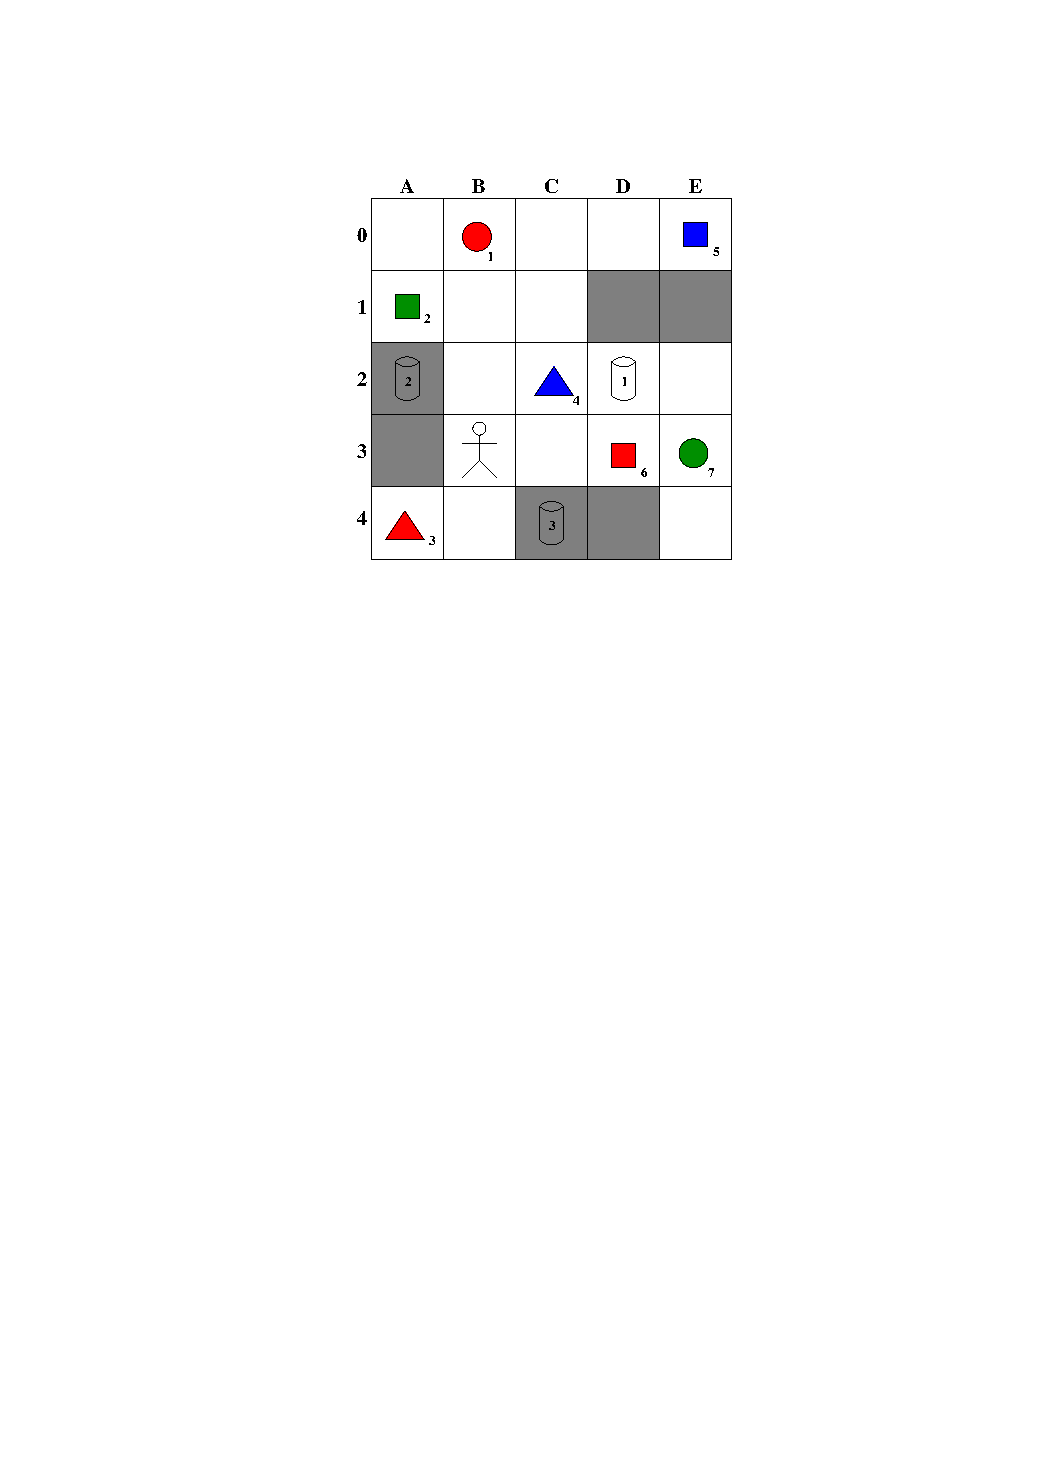
\includegraphics[width=.9\textwidth]{fig/roboschool-example.pdf}\\
			\end{column}
		\end{columns}
	\end{frame}
	
	\begin{frame}[c]\frametitle{Goals in PDDL}
		\begin{columns}
			\begin{column}[t]{0.3\textwidth}
			\lstinputlisting[basicstyle=\fontsize{5}{5.5}\selectfont,language=PDDL]{examples/pb1.pddl.txt}
			 			\lstinputlisting[basicstyle=\fontsize{5}{5.5}\selectfont,language=PDDL]{examples/pb1_plan.txt}
			\end{column}
			\begin{column}[t]{0.3\textwidth}
			\lstinputlisting[basicstyle=\fontsize{5}{5.5}\selectfont,language=PDDL]{examples/pb2.pddl.txt}
			 			\lstinputlisting[basicstyle=\fontsize{5}{5.5}\selectfont,language=PDDL]{examples/pb2_plan.txt}
			\end{column}
			\begin{column}[t]{0.3\textwidth}
			\lstinputlisting[basicstyle=\fontsize{5}{5.5}\selectfont,language=PDDL]{examples/pb3.pddl.txt}
			 			\lstinputlisting[basicstyle=\fontsize{5}{5.5}\selectfont,language=PDDL]{examples/pb3_plan.txt}
			\end{column}
		\end{columns}
		% \begin{columns}
% 			\begin{column}[t]{0.3\textwidth}
% 			\lstinputlisting[basicstyle=\fontsize{5}{5.5}\selectfont,language=PDDL]{examples/pb4.pddl.txt}
% 			 			\lstinputlisting[basicstyle=\fontsize{5}{5.5}\selectfont,language=PDDL]{examples/pb4_plan.txt}
% 			\end{column}
% 			\begin{column}[t]{0.3\textwidth}
% 			\lstinputlisting[basicstyle=\fontsize{5}{5.5}\selectfont,language=PDDL]{examples/pb5.pddl.txt}
% 			 			\lstinputlisting[basicstyle=\fontsize{5}{5.5}\selectfont,language=PDDL]{examples/pb5_plan.txt}
% 			\end{column}
% 			\begin{column}[t]{0.3\textwidth}
% 			\lstinputlisting[basicstyle=\fontsize{5}{5.5}\selectfont,language=PDDL]{examples/pb6.pddl.txt}
% 			 			\lstinputlisting[basicstyle=\fontsize{5}{5.5}\selectfont,language=PDDL]{examples/pb6_plan.txt}
% 			\end{column}
% 		\end{columns}
	\end{frame}
	
    \begin{frame}[c]\frametitle{Goal Recognition Problem}
		\begin{definition}[\textbf{Goal Recognition Problem}]
			A goal recognition problem is a tuple $P_{G} = \langle \Xi, \mathcal{I}, \mathcal{G}, \mathbf{O} \rangle$, where:
       	\begin{itemize}
       		\item $\Xi = \langle \Sigma, \mathcal{A} \rangle$ is the domain definition (facts and actions) ;
       		\item $\mathcal{I} \subseteq \Sigma$ is the initial state;
       		\item $\mathcal{G}$ s.t. $\forall{G \in \mathcal{G}}, G \subseteq \Sigma$ is a set of candidate goals (with an assumed hidden goal $G$); and
       		\item $\mathbf{O}$ is a sequence $\langle o_1, \dots o_n \rangle$ of observations, where $o_i \in \mathcal{A}$
       	\end{itemize}
       	\end{definition}
        
        \begin{itemize}
        	\item The solution for a goal recognition problem is the hidden goal $G \in \mathcal{G}$ that is most consistent with observation sequence $O$.
        	\item Caveat: we may have other representations for the observations
        	\item This is what I will refer to as PRAP
        \end{itemize}
    \end{frame}	
 
	\begin{frame}[c]\frametitle{Plan Recognition Problem}
		\begin{definition}[Plan Recognition Problem]
			A plan recognition problem is a tuple $P_{P} = \langle \Xi, \mathcal{M}, \mathcal{I}, \mathbf{O} \rangle$, where:
	       	\begin{itemize}
	       		\item $\Xi = \langle \Sigma, \mathcal{A} \rangle$ is the domain definition (facts and actions) ;
				\item $\mathcal{M}$ is a plan-library containing task-decomposing methods of the form $\langle t, \langle t_1, \dots t_n \rangle \rangle$ (implicitly defining a set $\mathcal{T}$ of task symbols); and
	       		\item $\mathcal{I} \subseteq \Sigma$ is the initial state;
	       		\item $\mathbf{O}$ is a sequence $\langle o_1, \dots o_n \rangle$ of observations, where $o_i \in \mathcal{A}$
	       	\end{itemize}
			Here, $\mathcal{T}$ comprises non-primitive tasks and primitive tasks corresponding to the names of actions $a \in \mathcal{A}$.
		\end{definition}
		
		\begin{itemize}
			\item The solution to a plan recognition goal is the top level task $t_{I} \in \mathcal{T}$ that generates a decomposition consistent with the observations in $\mathcal{O}$
			\item Requires a lot more domain knowledge (i.e. the plan-library)
			\item This is what I will refer to as classical plan recognition 
		\end{itemize}
	\end{frame}
	
	% \begin{frame}[c]\frametitle{Roboschool}
	% 	{\color{red} Add Roboschool problem for master class}
	% \end{frame}
	
	\begin{frame}[c]\frametitle{Observations}
		\begin{itemize}
			\item Observations often refer to \emph{observed action symbols}
			\begin{itemize}
				\item This observation sequence can be either \textbf{partial} or \textbf{full}
				\item Observation sequence can be \textbf{noisy}
				\item Observations can also be of \textbf{states/fluents} rather than actions
			\end{itemize}
		\end{itemize}
		\begin{columns}
			
			\begin{column}[t]{0.3\textwidth}
				{\color{red} Original Plan}\\
				\lstinputlisting[basicstyle=\fontsize{6}{6.5}\selectfont,language=PDDL]{examples/pb2_plan.txt}
			\end{column}
			\begin{column}[t]{0.6\textwidth}
				\only<2>{
				{\color{red} Full Observation}\\
				\lstinputlisting[basicstyle=\fontsize{6}{6.5}\selectfont,language=PDDL,linerange={1-15}]{examples/pb2_plan.txt}}
				\only<3>{
				{\color{red} Partial Observation}\\
				\lstinputlisting[basicstyle=\fontsize{6}{6.5}\selectfont,language=PDDL,linerange={1-1,4-5,8-9,13-15}]{examples/pb2_plan.txt}}
				\only<4>{
				{\color{red} Noisy Observation}\\
				\lstinputlisting[basicstyle=\fontsize{6}{6.5}\selectfont,language=PDDL,linerange={1-17}]{examples/pb2_plan-noisy.txt}}
				\only<5>{
				{\color{red} Noisy Partial Observation}\\
				\lstinputlisting[basicstyle=\fontsize{6}{6.5}\selectfont,language=PDDL,linerange={1-3,5-8,10-13,16-17}]{examples/pb2_plan-noisy.txt}}
				\only<6>{
				{\color{red} State Observation}\\
				\lstinputlisting[basicstyle=\fontsize{6}{6.5}\selectfont,language=PDDL]{examples/pb2_observation.txt}}
				\only<7>{
				{\color{red} Noisy State Observation}\\
				\lstinputlisting[basicstyle=\fontsize{6}{6.5}\selectfont,language=PDDL]{examples/pb2_observation-noisy.txt}}
			\end{column}
		\end{columns}
        
	\end{frame}
\fi

% @@@@@@@@@@@@@@@@@@@@@@@@@@@@@@@@@@@@@@@@@@@@@@@@@@@@@@@@@@@@@@@
	
\section{Goal Recognition as reasoning over Heuristics}

\subsection{Motivation and Background}
\if\masterclass1
	% \begin{frame}[c]\frametitle{Goal Recognition}
% 		Background on other PRAP approaches:
% 		\begin{itemize}
% 			\item Ramirez and Geffner
% 			\item Martin
% 			\item Sohrabi
% 		\end{itemize}
% 	\end{frame}
	\begin{frame}[c]\frametitle{Motivation}
		\begin{itemize}
			\item Plan Recognition as Planning (PRAP) requires much less domain knowledge  \\
			No need for a plan library
			\item Existing approaches are accurate, but very inefficient
			\item Key Insight: Landmark-based heuristics are efficient and informative\\
			\begin{itemize}
				\item landmarks provide evidence of \textbf{expected sequence} of observations
				\item can be computed once before recognition time
			\end{itemize}
		\end{itemize}
	\end{frame}
	
	\begin{frame}[c]\frametitle{Previous Work: Ramirez and Geffner (2009 and 2010)}
		\begin{itemize}
			\item First approaches to goal recognition: Plan Recognition as Planning (PRAP)
			\item Probabilistic model aims to compute $P(G \mid O)$
			\item Following Bayes Rule $P(G \mid O) = \alpha P(O \mid G) P(G)$
			\item Given $P(G)$ as a prior, key bottleneck is computing $P(O \mid G)$
			\begin{itemize}
				\item In their work $P(O \mid G)$ is computed in terms of a cost difference $c(G,O) - c(G,\bar{O})$
				\item Computational cost is \textbf{two planner calls per goal hypothesis}
				\item For online recognition: two planner calls per goal hypothesis \textbf{per observation}
			\end{itemize}
			\item Some conclusions challenged for path planning domains\\ (Masters and Sardina 2017)
		\end{itemize}
	\end{frame}
	\begin{frame}[c]\frametitle{Previous Work: E-Martín et al. (2015)}
		\begin{itemize}
			\item Improvement over Ramirez and Geffner's approach:
			\begin{itemize}
				\item Relaxes assumption that $c(G \mid O) < c(G,\bar{O})$
				\item Based on pre-computation of cost estimates using a planning graph
				\item Often orders of magnitude faster than Ramirez
			\end{itemize}
			\item Performance degrades substantially with low observability
			\item Does not cope with noisy observations
		\end{itemize}
	\end{frame}
	\begin{frame}[c]\frametitle{Previous Work: Sohrabi et al.}
		\begin{itemize}
			\item Formalizes PRAP with explicit assumptions and notions of 
			\begin{itemize}
				\item noisy observations
				\item incomplete observations
				\item action costs
			\end{itemize}
			\item Solves the goal recognition problem using a combination of:
			\begin{itemize}
				\item transformation of the recognition problem into a new $P'$ planning problem
				\item approximation of $P(G \mid O)$ by generating ``diverse plans'' for $P'$
			\end{itemize}
			\item Very accurate recognition for some domains
			\item No runtime efficiency evaluation (likely to be slow)
		\end{itemize}
	\end{frame}
\fi
	
    \begin{frame}{Overview}
       	\begin{itemize}
			\item In this work, we use a \textbf{planning domain definition} to represent agent behavior and environment properties;
			\item Previous approaches involve multiple calls to a modified planner.
			\item Our main contribution is twofold:
				\begin{itemize}
					\item We \textbf{obviate the need to execute a planner multiple times} for recognizing goals; and
					\item We develop novel goal recognition heuristics that \textbf{use planning landmarks}.
				 \end{itemize}
			% \item We evaluate our approaches against the fastest and most accurate approach of Ramírez and Geffner ({\footnotesize Plan Recognition as Planning. IJCAI, 2009}) over \textbf{15 planning domains};
			\item We show that our approaches are \textbf{more accurate} and \textbf{orders of magnitude faster} than Ramírez and Geffner's approach.
		\end{itemize}
    \end{frame}

\if\masterclass1
	

% \subsection{Planning Heuristics}
	
	% \begin{frame}[c]\frametitle{Solving Planning Problems}
	% 	Actions $a \in \mathcal{A}$ are tuples $a = \langle \mathit{name}, \mathit{pre}(a), \mathit{eff}(a), \mathit{cost}(a) \rangle$.
	% 	They induce a state transition system such that:
	% 	\begin{itemize}
	% 		\item $\mathit{eff}(a)$ constitute a set of negative (delete) and positive (add) effects: $\mathit{eff}^{+}(a)$, $\mathit{eff}^{-}(a)$
	% 		\item an action $a$ is applicable to a state $s$ iff $s \models \mathit{pre}(a)$
	% 		\item applying $a$ to $s$ ($\gamma(s,a)$) yields a state $s' = (s / \mathit{eff}^{-}(a)) \cup  \mathit{eff}^{+}(a)$, \\i.e. it is such that $s' \models \mathit{eff}(a)$
	% 	\end{itemize}
	% 	The solution to a planning problem $\Pi = \langle \Xi, \mathcal{I}, G\rangle$ is a plan $\pi = \langle a_1, \dots, a_n\rangle$ such that:
	% 	\begin{itemize}
	% 		\item $\mathcal{I} \models \mathit{pre}(a_1)$
	% 		\item $\gamma(\gamma(\dots \gamma(I, a_1),\dots), a_n) \models G$
	% 		\item The cost of $\pi$ is $\sum_{i=1}^{n}\mathit{cost}(a_i)$
	% 	\end{itemize}
	% \end{frame}
	
	\begin{frame}[c]\frametitle{From STRIPS Problem P to state model S(P)}
		Most modern planning algorithms convert a planning problem $\Pi = \langle \Xi, \mathcal{I}, G\rangle$, with $\Xi = \langle \Sigma, \mathcal{A} \rangle$ into one of state space search, where:
		\begin{itemize}
			\item the states $s \in S$ are \textbf{collections of atoms} from $\Sigma$
			\item the initial state $s_0 = I$
			\item the goal states $S_g$ are such that $\forall{s \in S_g} s \models G$
			\item the applicable actions for a state $s$ in $A(s)$ are actions from $a \in  \mathcal{A}$ such that $s \models \mathit{pre}(a)$
			\item the successor state $s' = (s / \mathit{eff}^{-}(a)) \cup  \mathit{eff}^{+}(a)$
			\item all action costs are assumed to be 1
		\end{itemize}
		How do we solve these problems?
	\end{frame}
	
	\begin{frame}[c]\frametitle{Heuristic Search Planning}
		\begin{itemize}
			\item Explicitly \textbf{searches} graph associated with model $S(P)$ with \textbf{heuristic} $h(s)$ that estimates cost from $s$ to goal
			\item \textbf{Key idea:} Heuristic $h$ extracted automatically from problem $\Pi$
			\item This is the mainstream approach in classical planning \\(and other forms of planning as well), \\ enabling the solution of problems over \textbf{huge spaces} 
		\end{itemize}
	\end{frame}
	
	\begin{frame}[c]\frametitle{Heuristic Graph Search}
		\begin{algorithmic}[1]
			\small
			\Function{graphSearch}{problem $p$, strategy $s$}
			\State{$\mathit{closed} \gets \{ \}$}\Comment{We now keep a list of explored states}
		    \State{$\mathit{frontier}.\Call{add}{new Node(\mathit{p.initial})}$}
			   \Loop
			      \If{$\mathit{frontier}$ is empty}
					\State{\textbf{return} $\mathbf{fail}$}
				  \EndIf
				  \State{$n \gets s.\Call{removeChoice}{\mathit{frontier}}$}
				  \State{$\mathit{closed}.\Call{add}{n.state}$}\Comment{Where we keep states we already visisted}
				  \If{$\Call{p.goalTest}{\mathit{n.state}}$}
					\State{\textbf{return} $\Call{getPath}{n}$}
				  \EndIf
				  \ForAll{$a \in p.\Call{actions}{n}$}
				    \State{$n' \gets a.\Call{result}{\mathit{n.state}}$}
				    \If{$\mathit{n'.state} \notin \mathit{closed}$}
					\State{$\mathit{frontier}.\Call{add}{n'}$} \Comment{And only explore states we haven't visited}
					\EndIf
				  \EndFor
			   \EndLoop
			\EndFunction
		\end{algorithmic}
	\end{frame}
	
	\begin{frame}[c]\frametitle{Heuristics}
		\begin{itemize}
			\item A heuristic function \textbf{estimates} the true cost of reaching a goal $G$
			\item Only requirement for an heuristic $h(n)$ to \textbf{work} with $A^{*}$ is that $h(G)=0$
			\begin{itemize}
				\item Though this is \textbf{not} necessarily \textbf{optimal}
			\end{itemize}
		\end{itemize}
	\end{frame}

\newcommand\puzzle[9]{
			{\Large
			\begin{tabular}{|m{.5em}|m{.5em}|m{.5em}|}
			\hline
			#1 & #2 & #3\\
			\hline
			#4 & #5 & #6\\
			\hline
			#7 & #8 & #9\\
			\hline
			\end{tabular}
			}
}

	\begin{frame}[c]\frametitle{Heuristic Functions}
		\begin{columns}
		\begin{column}{0.5\textwidth}
			\begin{center}
				\puzzle{7}{2}{4}
				       {5}{ }{6} 
				       {8}{3}{1}\\[1em]
				Start State
			\end{center}
		\end{column}
		\begin{column}{0.5\textwidth}
			\begin{center}
				\puzzle{1}{2}{3}
				       {4}{5}{6} 
				       {7}{8}{ }\\[1em]
				Goal State
			\end{center}
		\end{column}
		\end{columns}
		\begin{itemize}
			\item Heuristics
			\begin{itemize}
				\item<2-> The number of misplaced tiles -- \textbf{Hamming distance} ($h_1 = 7$)
				\item<2-> The sum of distances of the tiles from their goal positions -- \textbf{Manhattan distance} ($h_2 = 16$)  
			\end{itemize}
			\item<2-> Are they admissible?
		\end{itemize}
	\end{frame}

	\begin{frame}[c]\frametitle{Creating Heuristics}
		\begin{itemize}
			\item Ignore specific preconditions of actions (need some domain knowledge)
			\item Consider the sliding blocks from search
		\end{itemize}
		\lstinputlisting[basicstyle=\fontsize{8}{8.5}\selectfont,language=PDDL]{examples/sliding_blocks.pddl.txt}
		\begin{itemize}
			\item If we remove \texttt{(blank s2)}, we are left with Manhattan distance
		\end{itemize}
	\end{frame}
	
	\begin{frame}[c]\frametitle{Domination}
		\begin{itemize}
			\item h2 is always greater than h1. 
			\begin{itemize}
				\item It therefore dominates h1 (it is a tighter bound on the actual cost)
				\item And is more efficient
			\end{itemize}
			\item How can we invent good heuristics?
			\item Typically, by \textbf{relaxing} the problem.
		\end{itemize}
	\end{frame}

	\begin{frame}[c]\frametitle{Heuristics for Classical Planning}
		\begin{itemize}
			\item Key development in planning in the 90’s, is automatic extraction of \textbf{heuristic functions} to guide search for plans 
			\item The general idea was known: heuristics often \textbf{explained} as \textbf{optimal} cost functions of \textbf{relaxed} (simplified) problems (Minsky 61; Pearl 83)
			\item Most common relaxation in planning, $P^+$, obtained by dropping \textbf{delete-lists} from ops in P. If $c^*(P)$ is optimal cost of P, then
			$$h^{+}(P) \myeq c^{*}(P^{+})$$
			\item Heuristic $h^{+}$ \textbf{intractable} but easy to \textbf{approximate}; i.e. 
			\begin{itemize}
				\item computing \textbf{optimal} plan for $P^{+}$ is \textbf{intractable}, but 
				\item computing a non-optimal plan for $P^{+}$ \textbf{(relaxed plan)} easy 
			\end{itemize}
			\item State-of-the-art heuristics as in FF or LAMA still rely on $P^{+}$
		\end{itemize}
	\end{frame}
	
	\begin{frame}[c]\frametitle{Additive Heuristic}
		\begin{itemize}
			\item For all \textbf{atoms} $p$:
			$$h(p;s) \myeq \begin{cases}
							0 & \mathit{if} p \in s, \mathit{else} \\
							\min_{a \in O}\left[ \mathit{cost}(a) + h(Pre(a); s) \right]
							\end{cases}$$
			\item For \textbf{sets} of atoms $C$, assume \textbf{independence}:
			$$h(C;s) \myeq \sum_{r \in C} h(r; s)$$
			\item Resulting \textbf{heuristic function} $h_{add}(s)$:
			$$h_{\mathit{add}}(s) \myeq h(Goal; s)$$
			\item Heuristic not admissible, but informative and fast
		\end{itemize}
	\end{frame}
	
	\begin{frame}[c]\frametitle{Max Heuristic}
		\begin{itemize}
			\item For all \textbf{atoms} $p$:
			$$h(p;s) \myeq \begin{cases}
							0 & \mathit{if} p \in s, \mathit{else} \\
							\min_{a \in O}\left[ 1 + h(Pre(a); s) \right]
							\end{cases}$$
			\item For \textbf{sets} of atoms $C$, assume \textbf{independence}:
			$$h(C;s) \myeq \max_{r \in C} h(r; s)$$
			\item Resulting \textbf{heuristic function} $h_{add}(s)$:
			$$h_{\mathit{max}}(s) \myeq h(Goal; s)$$
			\item Heuristic admissible, but not very informative
		\end{itemize}
	\end{frame}
	
	\begin{frame}[c]\frametitle{Max Heuristic and (Relaxed) Planning Graph}
		\begin{itemize}
			\item Build reachability graph $P_0, A_0, P_1, A_1, \dots$
		\end{itemize}
		\begin{center}
		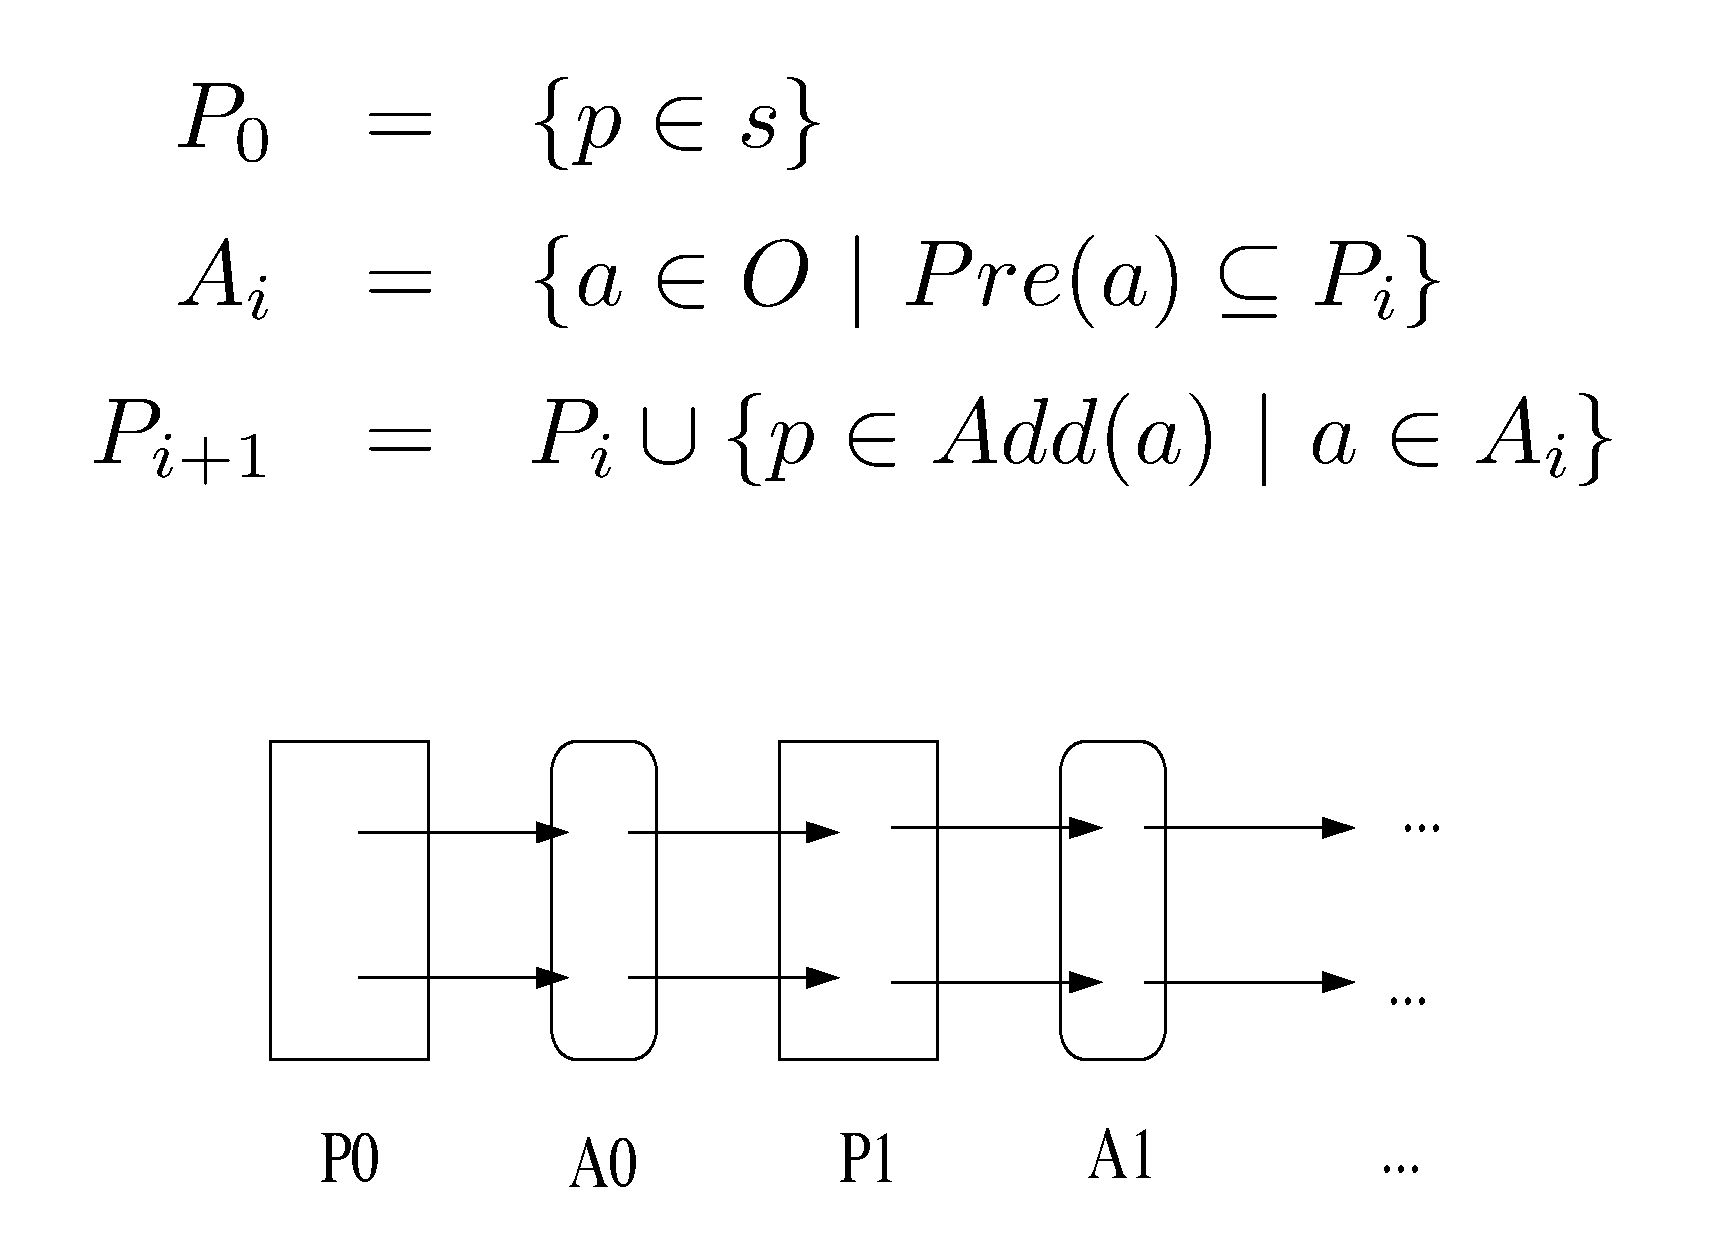
\includegraphics[width=.5\textwidth]{fig/rpg-example.pdf}
		\end{center}
		\begin{itemize}	
			\item Graph implicitly \textbf{represents} max heuristic
			$$h_{\mathit{max}}(s) = \min~i~\mathit{such~that}~G \subseteq P_{i}$$
		\end{itemize}
	\end{frame}
	
	\begin{frame}[c]\frametitle{Relaxed Planning Graph}
		\begin{itemize}
			\item A variation of the Planning Graph from Graphplan
			\begin{itemize}
				\item Alternating fact and action levels
				\item Ignores negative effects from actions, no mutex relations
			\end{itemize}
			\item Fact level $F_0$ contains the facts that are true in the initial state, 
			\item Action level $A_0$ contains actions whose preconditions are reached from $F_0$,
			\item $F_1$ contains $F_0$ plus the add effects of the actions in $A_0$, and so on.
		\end{itemize}
	\end{frame}

	\begin{frame}[c]\frametitle{RPG Construction}
		\begin{algorithmic}[1]
			\small
		    \Function{BuildFullRPG}{$\Xi$, $\mathcal{I}$, $G$}
		    		\State $i \gets 0$
		    		\State \textsc{RPG.FactLevel$_{0}$} $\gets \mathcal{I}$
		    		\While{$G \nsubseteq$ \textsc{RPG.FactLevel$_{i}$}}
		    			\State \textsc{RPG.ActionLevel$_{i}$} $\gets \lbrace a \in \mathcal{A} \mid$ \textit{pre}($a$) $\in$ \textsc{RPG.FactLevel$_{i}$}$\rbrace$
		    			\State \textsc{RPG.FactLevel$_{i+1}$} $\gets$ \textsc{RPG.FactLevel$_{i}$} $\cup$ \textit{eff}($a$)$^+$, $\forall a \in$ \textsc{RPG.ActionLevel$_{i}$}
					\If{\textsc{RPG.FactLevel$_{i+1}$} $\equiv$ \textsc{RPG.FactLevel$_{i}$}}
						\State \textbf{return} $G$ \textsc{unreachable} \Comment{\textit{The algorithm fails if at some point before reaching the facts of the goal no new fact level is added in the graph.}}
					\EndIf
		    			\State $i \gets i + 1$
		    		\EndWhile
		        \State \textbf{return} \textsc{RPG}
		    \EndFunction
		\end{algorithmic}
	\end{frame}
	
	\begin{frame}[c]\frametitle{Blocks World: RPG}
		\begin{center}
			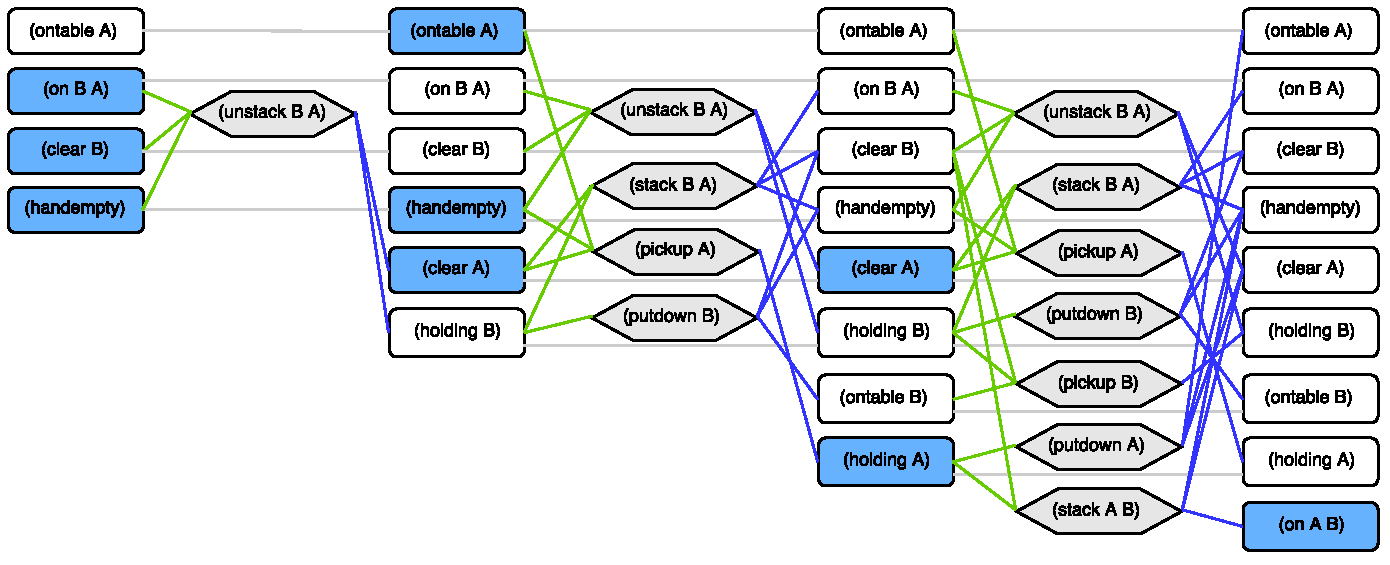
\includegraphics[width=\textwidth]{fig/blocksworld-landmarks-rpg.pdf}
		\end{center}
		\vspace{-2cm}
		Blocks World Problem\\
		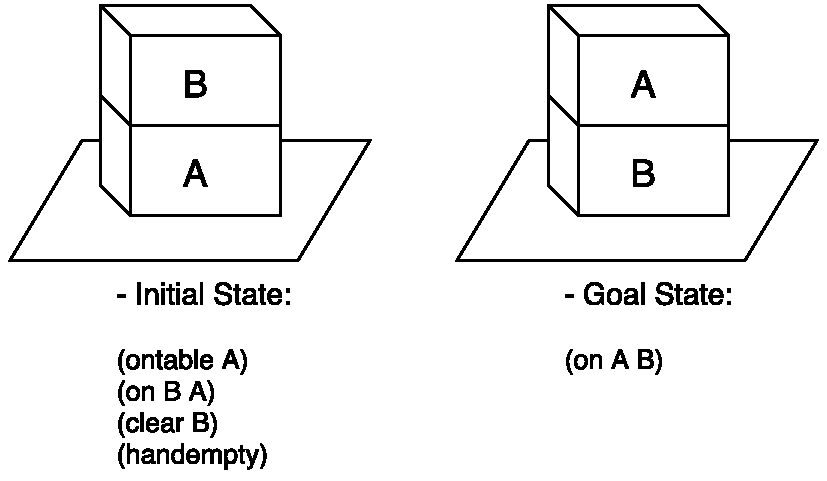
\includegraphics[width=.5\textwidth]{fig/blocksworld-problem.pdf}
	\end{frame}

\subsection{Estimating Goal Completion with Landmarks}
	
    \begin{frame}{Background: Planning and Landmarks}
		\begin{definition} [\textbf{Planning}]
			A planning instance is represented by a triple $\Pi = \langle \Xi, \mathcal{I}, G\rangle$, in which:
			\begin{itemize}
				\item $\Xi$ $=$ $\langle$$\Sigma$, $\mathcal{A}$$\rangle$ is the \textbf{domain definition}, and consists of a finite set of \textbf{facts} $\Sigma$ and a finite set of \textbf{actions} $\mathcal{A}$ (action costs $=$ 1);
				\item $\mathcal{I}$ and $G$ represent the \textbf{planning problem}, in which $\mathcal{I}$ $\subseteq$ $\Sigma$ is the \textbf{initial state}, and $G$ $\subseteq$ $\Sigma$ is the \textbf{goal state}.
			\end{itemize}
		\end{definition}
		\begin{definition}[\textbf{Landmarks}]
			Given a planning instance $\Pi = \langle \Xi, \mathcal{I}, G\rangle$, a \textbf{fact} (or \textbf{action}) $L$ is a landmark in $\Pi$ iff $L$ 	must be \textbf{satisfied} (or \textbf{executed}) at some point along all valid plans that achieve $G$ from $\mathcal{I}$.
		\end{definition}
		% \begin{itemize}
% 			\item To extract landmarks and their ordering, we use an algorithm developed by Hoffman \emph{et al.} {\footnotesize (Ordered Landmarks in Planning. JAIR, 2004)}.
% 		\end{itemize}
    \end{frame}
	
	\begin{frame}[c]\frametitle{Computing Landmarks}
		\begin{itemize}
			\item Deciding whether a fact is a landmark is PSPACE-complete\\
				Involves deciding whether a plan exists with out actions that achieve it
			\item Multiple types of landmarks/orderings
			\item Multiple ways of computing landmarks:
			\begin{itemize}
				\item Complete set of landmarks (very expensive)
				\item Various methods to compute incomplete set of landmarks \\(e.g. delete relaxation, backchaining on RPG)
				\item Disjunctive landmarks
			\end{itemize}
			\item In our work we use an algorithm from Hoffman \emph{et al.} (2004) to compute an incomplete set of landmarks with a partial order relation
		\end{itemize}
	\end{frame}
	
	\begin{frame}[c]\frametitle{Computing Landmarks}
		% \begin{columns}
% 			\begin{column}{0.5\textwidth}
% 			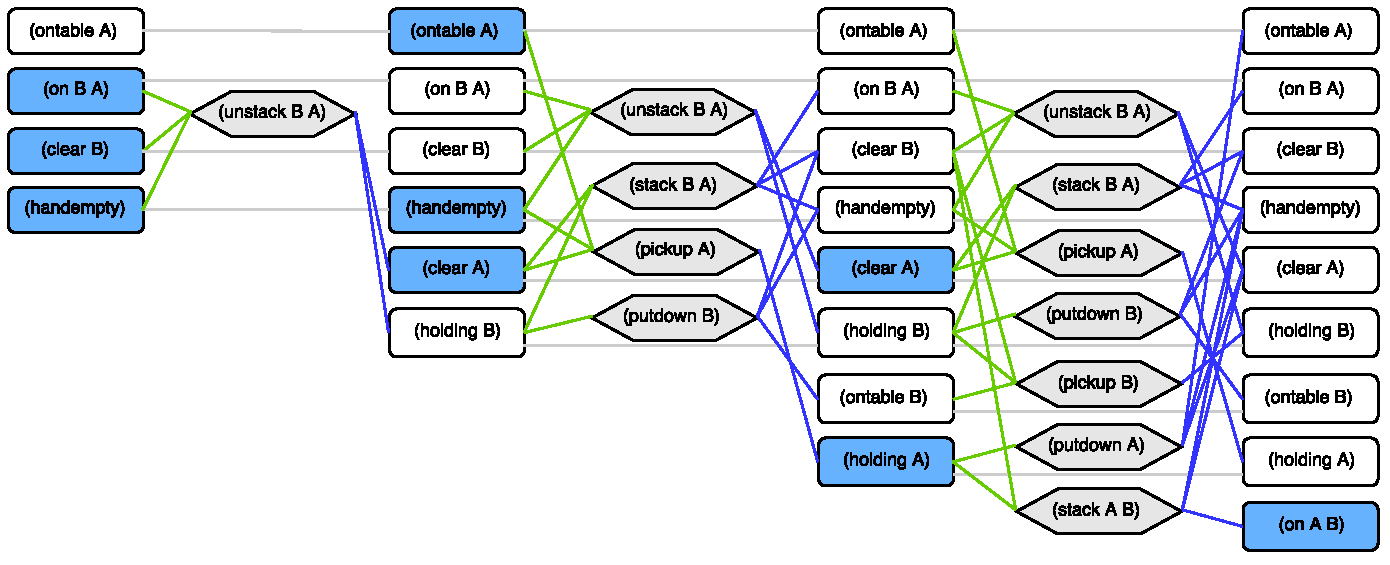
\includegraphics[width=\textwidth]{fig/blocksworld-landmarks-rpg.pdf}
% 			\end{column}
% 		\begin{column}{0.5\textwidth}
% 			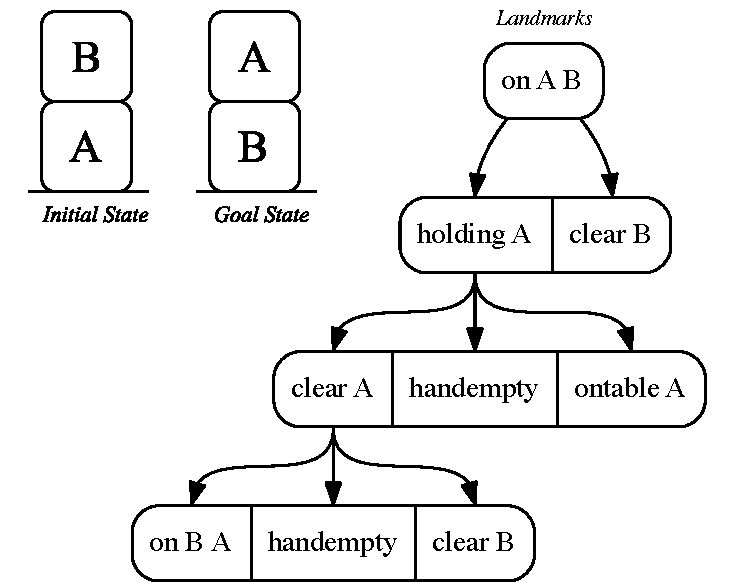
\includegraphics[width=\textwidth]{fig/blocksworld-landmarks-example.pdf}
% 		\end{column}
% 		\end{columns}

		\begin{center}
			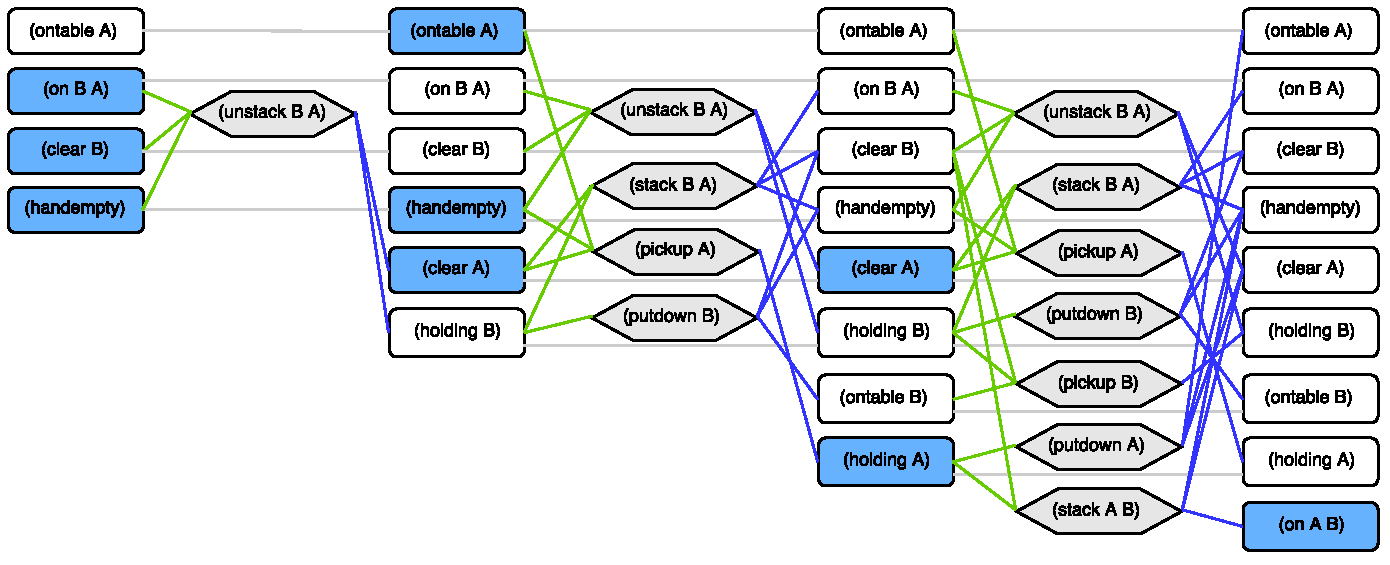
\includegraphics[width=\textwidth]{fig/blocksworld-landmarks-rpg.pdf}
		\end{center}
		\vspace{-2cm}
		Blocks World Problem\\
		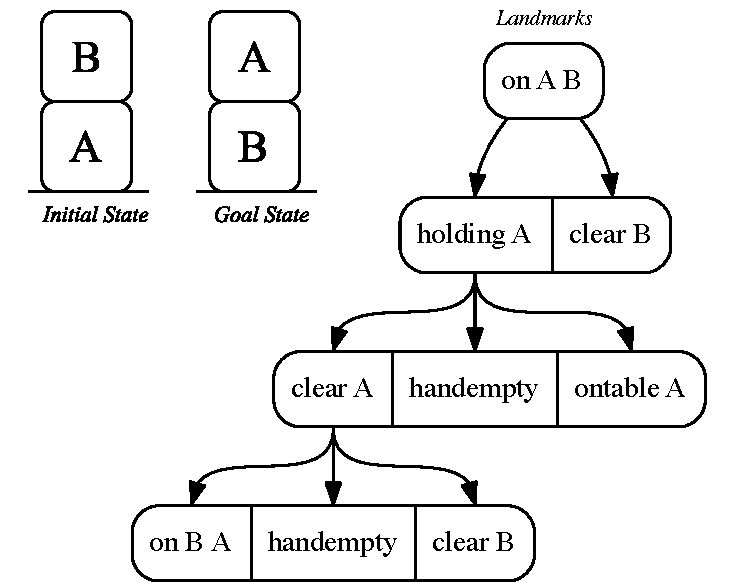
\includegraphics[width=.4\textwidth]{fig/blocksworld-landmarks-example.pdf}
	\end{frame}
\fi


%---------------------------------------------------------------------------------

    \begin{frame}{Computing Achieved Landmarks}
		\if\masterclass1
		% \todo{Change this example to the one from Ramirez}
		\fi
		\begin{center}
		    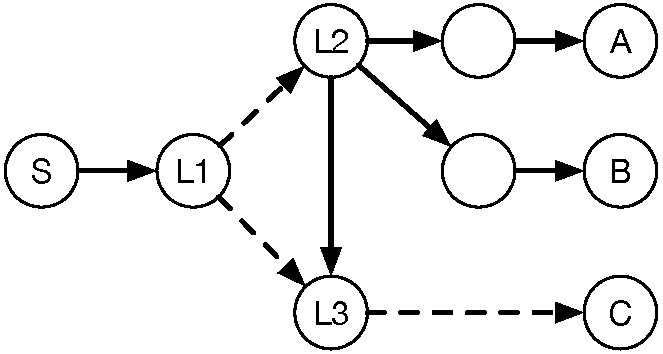
\includegraphics[width=.4\textwidth]{example.pdf} 
		\end{center}
		
       	\begin{itemize}
       		\item Our heuristics require identifying which fact landmarks have been achieved during the observed plan execution for every candidate goal $G \in \mathcal{G}$;
            \item For every candidate goal $G \in \mathcal{G}$:
            	\begin{itemize}
                	\item Extract \emph{ordered} landmarks for $G$;
                    \item Use achieved landmarks of $G$ in preconditions and effects of every observed action $o \in O$;
                   \item Under partial observability, we deal with missing actions by inferring that predecessors of observed landmarks must have been achieved;
                \end{itemize}
		\end{itemize}
% 		\begin{figure}[here]
% 			\centering
% 			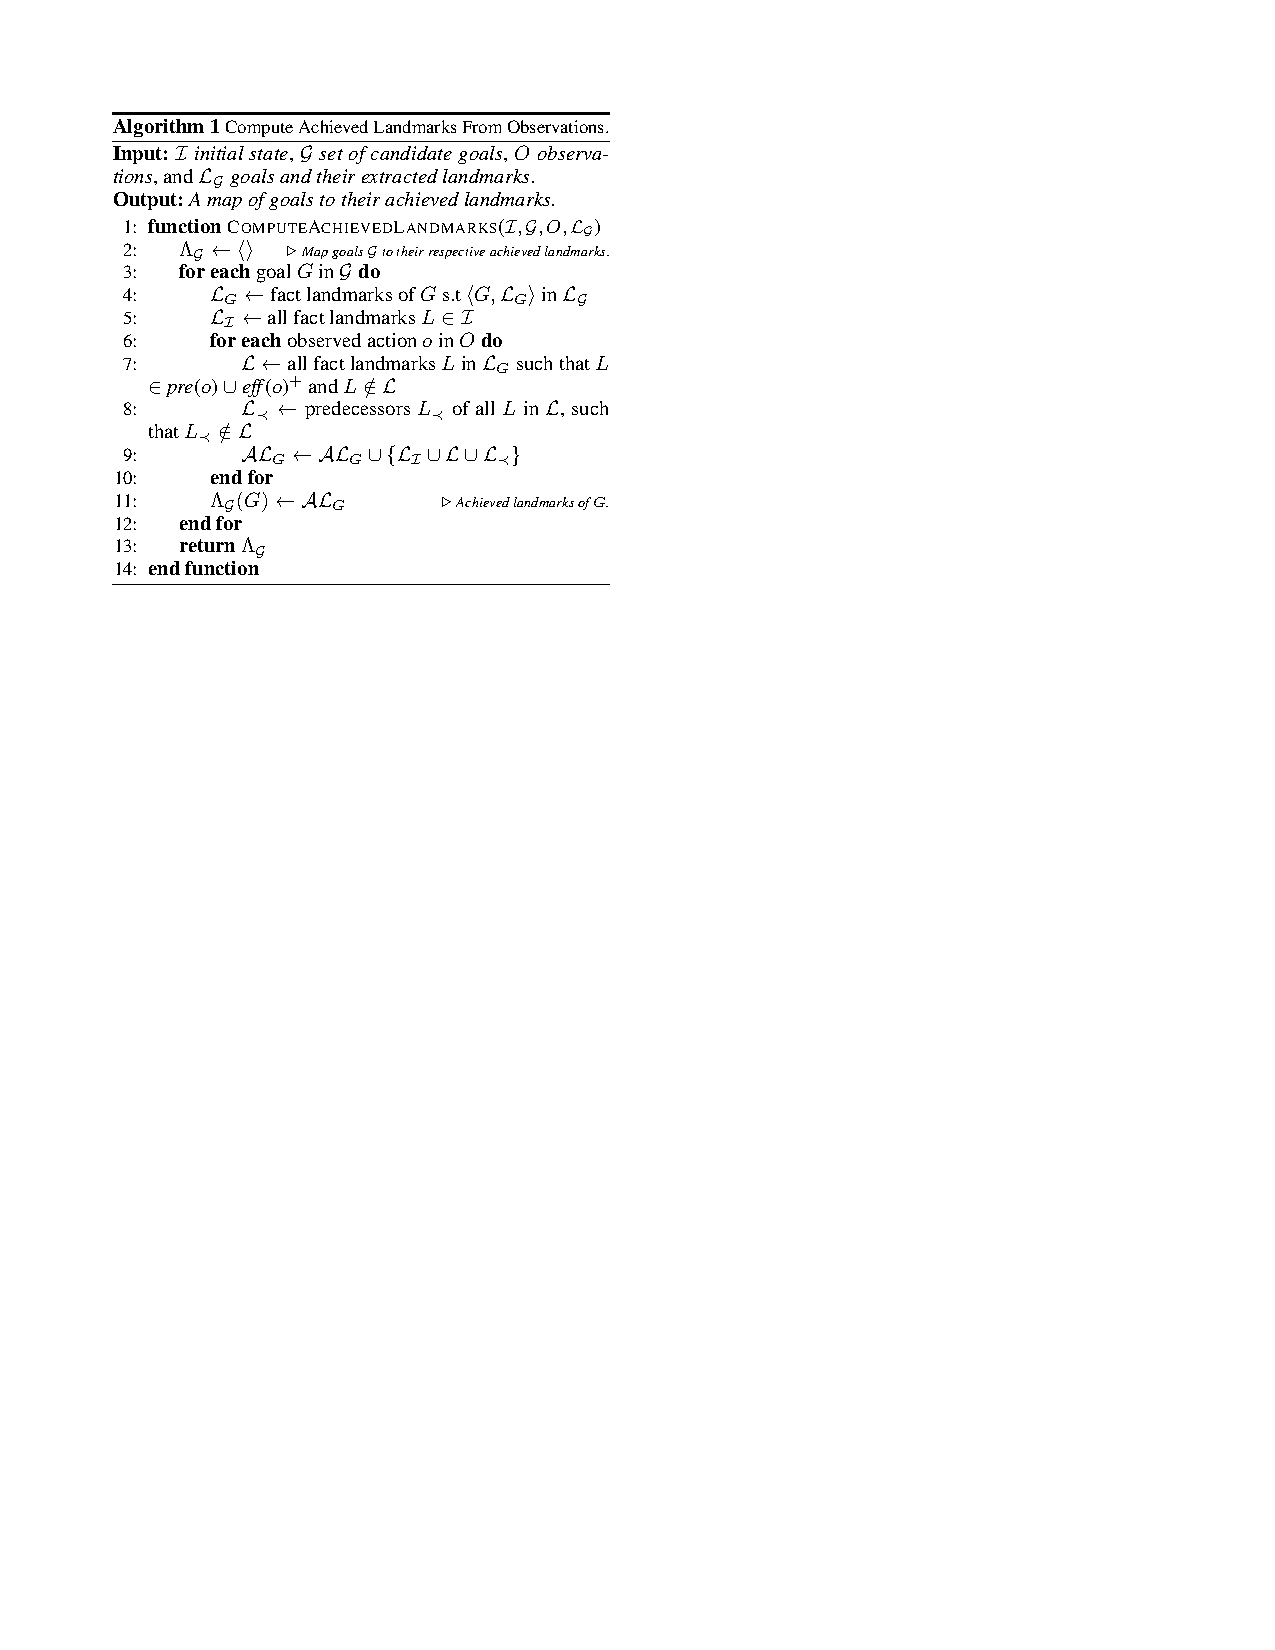
\includegraphics[width=0.65\linewidth]{algo1-computing_achieved_landmarks.pdf}
% 		\end{figure}
    \end{frame}
	
%---------------------------------------------------------------------------------

    \begin{frame}{Landmark-Based Goal Completion Heuristic}
       	\begin{itemize}
       		\item Goal Completion $h_{gc}$ aggregates the percentage of completion of each sub-goal into an overall percentage of completion for all facts of a candidate goal;
		\end{itemize}
		
		\begin{equation}
			h_{gc}(G, \mathcal{AL}_{G}, \mathcal{L}_{G}) = \left(\frac{\sum_{g \in G} \frac{|\mathcal{AL}_{g} \in \mathcal{AL}_{G} |}{|\mathcal{L}_{g} \in \mathcal{L}_{G}|}}{ |G| }\right)
		\end{equation}
		where:
		\begin{itemize}
			\item $\mathcal{AL}_{G}$ achieved landmarks for goals in $G$
			\item $\mathcal{L}_{G}$ all landmarks for goals in $G$
		\end{itemize}
    \end{frame}
	
% @@@@@@@@@@@@@@@@@@@@@@@@@@@@@@@@@@@@@@@@@@@@@@@@@@@@@@@@@@@@@@@

\if\masterclass1
    \begin{frame}{Landmark-Based Goal Completion Heuristic: Algorithm}
		\begin{itemize}
			\item Our approach allows the use of a threshold $\theta$, giving us \textbf{flexibility to avoid eliminating candidate goals} whose the percentage of goal completion are close to the highest completion value;
		\end{itemize}
		
		\begin{figure}[here]
			\centering
			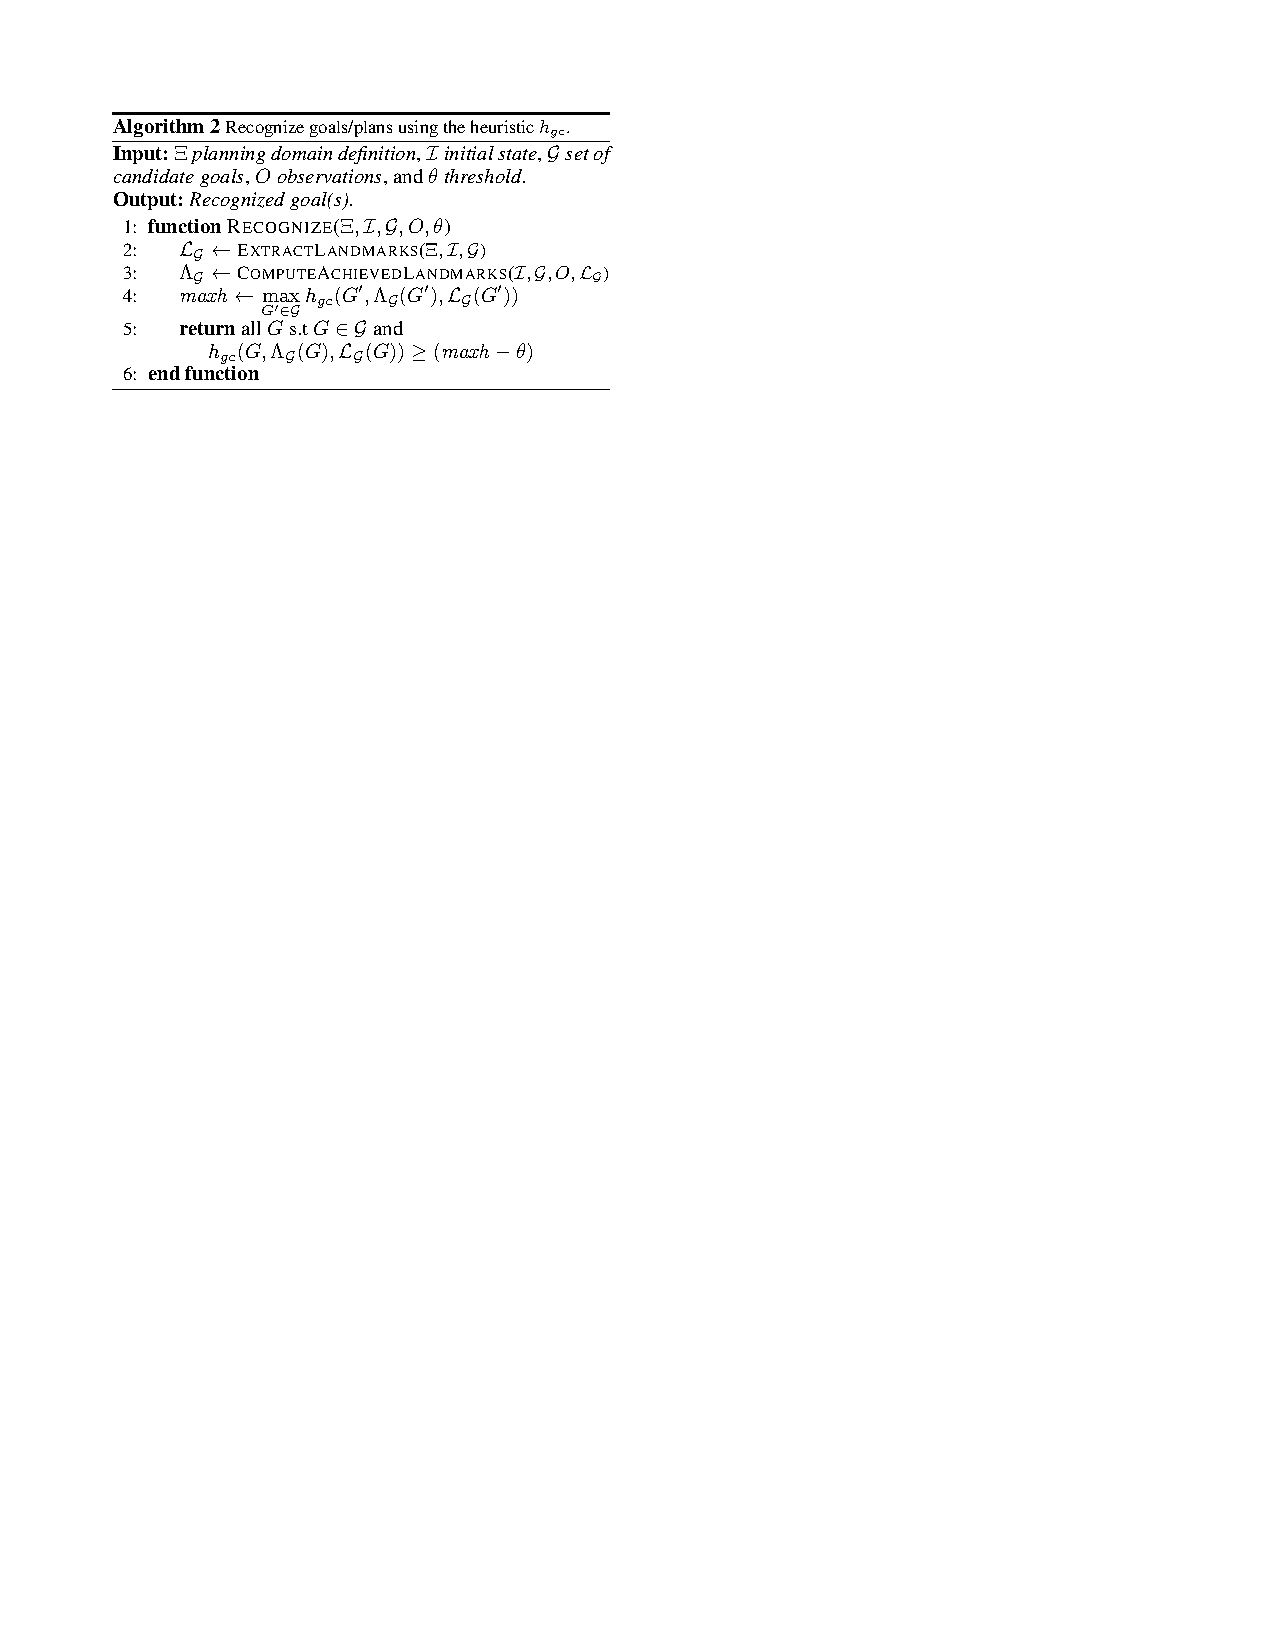
\includegraphics[width=0.8\linewidth]{algo2-heuristic_goalcompletion.pdf}
		\end{figure}	
	\end{frame}	
\fi

%---------------------------------------------------------------------------------

    \begin{frame}{Landmark-Based Uniqueness Heuristic (1 of 2)}
       	\begin{itemize}
       		\item Our second heuristic computes \textbf{landmark uniqueness}: \\inverse frequency of a landmark within landmarks for candidate goals:%, \emph{i.e.}, how unique (and thus informative) each landmark is among all landmarks; 
		\end{itemize}
		
		\begin{equation}
			L_{\mathit{Uniq}}(L, \mathcal{L}_{\mathcal{G}}) = \left(\frac{1}{\displaystyle\sum_{\mathcal{L} \in \mathcal{L_G}} |\{L |L \in \mathcal{L}\}|}\right)
		\end{equation}
		
		\begin{center}
		    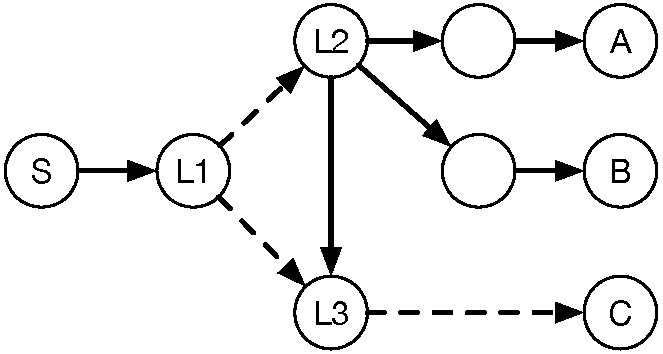
\includegraphics[width=.4\textwidth]{example.pdf} 
			\quad
			\begin{minipage}{.4\textwidth}
				\vspace{-6em}
			  $L_{\mathit{Uniq}}(L2)=1/2$ \\
			  $L_{\mathit{Uniq}}(L1)=1/3$ \\
			  $L_{\mathit{Uniq}}(L3)=1$
			\end{minipage}
		\end{center}
    \end{frame}
	
% @@@@@@@@@@@@@@@@@@@@@@@@@@@@@@@@@@@@@@@@@@@@@@@@@@@@@@@@@@@@@@@
	
	\begin{frame}{Landmark-Based Uniqueness Heuristic (2 of 2)}
		
		\begin{itemize}
			\item Our second heuristic, called $h_{uniq}$, estimates the goal completion of a candidate goal $G$ by calculating the ratio between the sum of the uniqueness value of the achieved landmarks of $G$ and the sum of the uniqueness value of all landmarks of $G$;
		\end{itemize}
		
		\begin{equation}
		h_{\mathit{uniq}}(G, \mathcal{AL}_{G}, \mathcal{L}_{G}, \Upsilon_{uv}) = \left(
		\frac
		{\displaystyle\sum_{\mathcal{A}_{L} \in \mathcal{AL}_{G}}\Upsilon_{uv}(\mathcal{A}_{L})}
		{\displaystyle\sum_{L \in \mathcal{L}_{G}}\Upsilon_{uv}(L)}\right)
		\end{equation}	
		
		where:
		\begin{itemize}
			\item $\Upsilon_{uv}$ is a table of uniqueness values
			\item $\mathcal{AL}_{G}$ achieved landmarks for goals in $G$
			\item $\mathcal{L}_{G}$ all landmarks for goals in $G$
		\end{itemize}
		
	\end{frame}
		
% @@@@@@@@@@@@@@@@@@@@@@@@@@@@@@@@@@@@@@@@@@@@@@@@@@@@@@@@@@@@@@@

\if\masterclass1
    \begin{frame}{Landmark-Based Uniqueness Heuristic: Algorithm}
       	\begin{itemize}
       		\item Our second heuristic is called $h_{uniq}$; 
		\end{itemize}
		
		\begin{figure}[here]
			\centering
			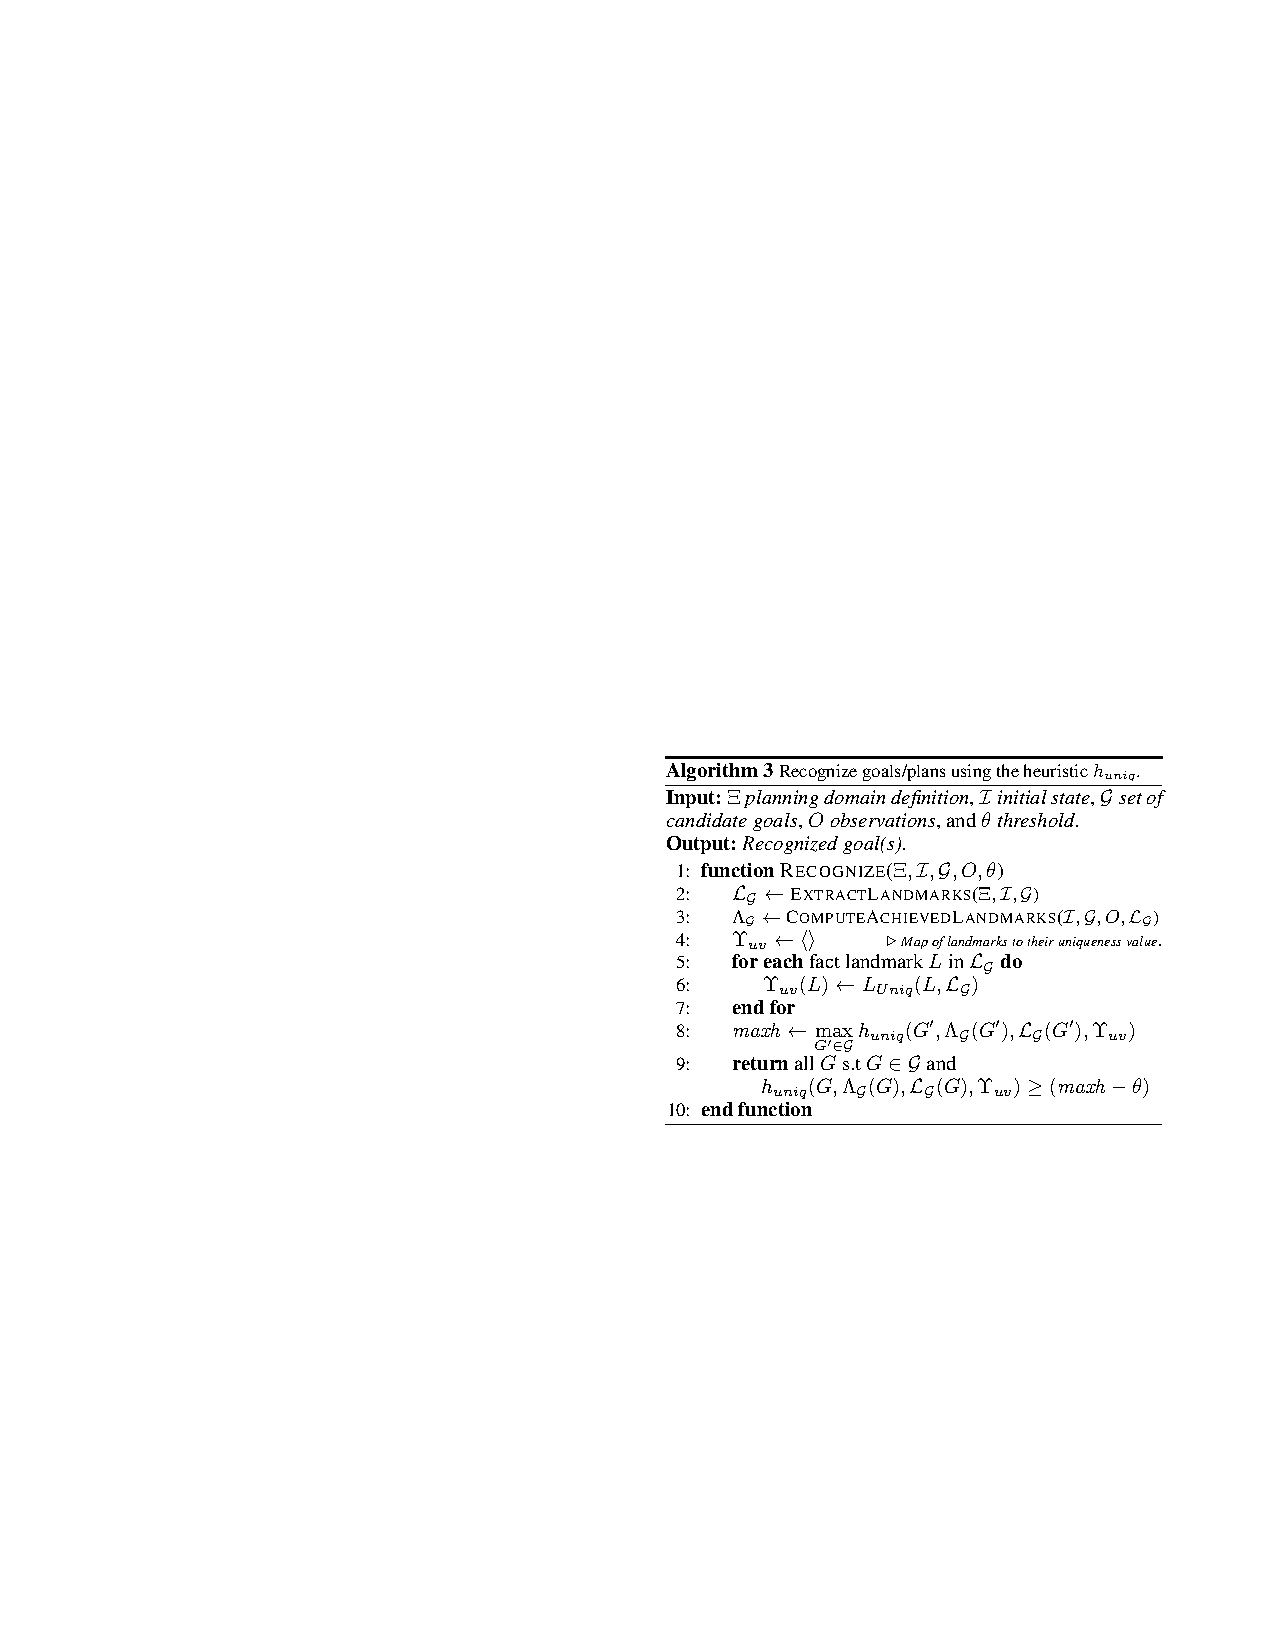
\includegraphics[width=0.75\linewidth]{algo3-heuristic_uniqueness.pdf}
		\end{figure}			
    \end{frame}	
\fi
%---------------------------------------------------------------------------------

% \if\masterclass1
    \begin{frame}{Example (1 of 4)}
		\begin{figure}[here]
			\centering
			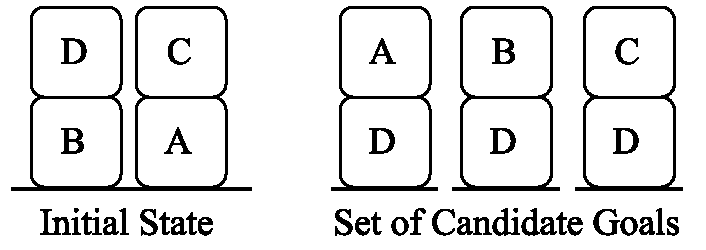
\includegraphics[width=0.75\linewidth]{example-blocksworld.pdf}
		\end{figure}
       	\begin{itemize}
       		\item Observations:
				\begin{itemize}
					\item \texttt{(unstack D B)}; and
					\item \texttt{(unstack C A)}.
				\end{itemize}
			\item The real goal is: \texttt{(and (ontable D) (on C D) (clear C))}
		\end{itemize}
    \end{frame}

\newcommand{\achieved}[1]{{\color{red}#1}}

    \begin{frame}{Example (2 of 4)}
		\textbf{Achieved Landmarks in Observations:}
       	\begin{itemize}
       		\item \texttt{(and (ontable D) (clear A) (on A D))}:%, 5 out of 8:
				\begin{itemize}\scriptsize \setlength{\itemindent}{-3em}
					% \item {\scriptsize \texttt{[(clear A)]}, \texttt{[(clear A) (ontable A) (handempty)]},
% 					\\ \texttt{[(on C A) (clear C) (handempty)]}, \texttt{[(holding D)]},
% 					\\ \texttt{[(clear D) (on D B) (handempty)]}}
					\item[] \texttt{(clear a) $\rightarrow$ \achieved{[(on c a), (clear c), (handempty)]}, \achieved{[(clear a)]}}, % 2 achieved 
					\item[] \texttt{(on a d) $\rightarrow$ \achieved{[(on c a), (clear c), (handempty)]}, \break \achieved{[(clear a), (ontable a), (handempty)]}, \break [(holding a), (clear d)], [(on a d)]}, % 2 achieved
					\item[] \texttt{(ontable d) $\rightarrow$ \achieved{[(clear d), (on d b), (handempty)]}, \achieved{[(holding d)]}, \break [(ontable d)]} % 2 achieved
				\end{itemize}
				
			\item \texttt{(and (ontable D) (clear B) (on B D)), 4 out of 7}:
				\begin{itemize}\scriptsize \setlength{\itemindent}{-3em}
					% \item {\scriptsize \texttt{[(clear B)]}, \texttt{[(ontable B) (handempty)]},
% 					\\ \texttt{[(on D B) (clear D) (handempty)]}, \texttt{[(holding D)]}}
					\item[] \texttt{(clear b) $\rightarrow$ \achieved{[(clear d), (on d b), (handempty)]}, \achieved{[(clear b)]}} % 2 achieved
					\item[] \texttt{(on b d) $\rightarrow$ \achieved{[(ontable b), (handempty)]}, [(clear d), (holding b)], [(on b d)]} % 1 achieved 
					\item[] \texttt{(ontable d) $\rightarrow$ \achieved{[(clear d), (on d b), (handempty)]}, \achieved{[(holding d)]}, \break [(ontable d)]} % 2 achieved
				\end{itemize}
			
			\item \texttt{(and (ontable D) (clear C) (on C D)), 5 out of 7}:
				\begin{itemize}\scriptsize \setlength{\itemindent}{-3em}
					% \item {\scriptsize \texttt{[(clear C)]}, \texttt{[(clear C) (on C A) (handempty)]}, \texttt{[(clear D) (holding C)]}
% 					\\ \texttt{[(clear D) (on D B) (handempty)]}, \texttt{[(holding D)]}}
					\item[] \texttt{(on c d) $\rightarrow$ \achieved{[(on c a), (clear c), (handempty)]}, \achieved{[(holding c), (clear d)]}, [on c d]} % 2 achieved
					\item[] \texttt{(ontable d) $\rightarrow$ \achieved{[(clear d), (on d b) (handempty)]}, \achieved{[(holding d)]}, [ontable d]} % 2 achieved 
					\item[] \texttt{(clear c) $\rightarrow$ \achieved{[(clear c)]}} % 1 achieved
				\end{itemize}
		\end{itemize}
    \end{frame}

    \begin{frame}{Example (3 of 4) - $h_{gc}$}
		\textbf{Landmark-Based Goal Completion Heuristic}
		% TODO break this down in more detail
       	\begin{itemize}
       		\item \texttt{(and (ontable D) (clear A) (on A D))}:%, 5 out of 8:
				\begin{itemize}
					%\item Goal Completion: 0.7222
					\item Goal Completion: $\displaystyle \frac{\frac{2}{2}+\frac{2}{4}+\frac{2}{3}}{3} =  0.7222$
				\end{itemize}
			\item \texttt{(and (ontable D) (clear B) (on B D))}:%, 4 out of 7:
				\begin{itemize}
					\item Goal Completion: $\displaystyle \frac{\frac{2}{2}+\frac{1}{3}+\frac{2}{3}}{3} =  0.6666$
				\end{itemize}
			\item \texttt{(and (ontable D) (clear C) (on C D))}:%, 5 out of 7:
				\begin{itemize}
					\item Goal Completion: $\displaystyle \frac{\frac{2}{3}+\frac{2}{3}+\frac{1}{1}}{3} =  0.7733$ \textbf{(highest estimated value)}
				\end{itemize}
		\end{itemize}
    \end{frame}

    \begin{frame}{Example (4 of 4) - $h_{uniq}$}
		\textbf{Landmark-Based Uniqueness Heuristic}
       	\begin{itemize}
       		\item \texttt{(and (ontable D) (clear A) (on A D))}, Total$_{Uniq}$ = 5.5:
				\begin{itemize}
					\item {\scriptsize \texttt{[(clear A)] = 1}, \texttt{[(clear A) (ontable A) (handempty)] = 1},
					\\ \texttt{[(on C A) (clear C) (handempty)] = 0.5}, \texttt{[(holding D)] = 0.3333},
					\\ \texttt{[(clear D) (on D B) (handempty)] = 0.3333}}
					\item $h_{uniq}$ = 3.1666 / 5.5 = 0.5757
				\end{itemize}
			\item \texttt{(and (ontable D) (clear B) (on B D))}, Total$_{Uniq}$ = 5:
				\begin{itemize}
					\item {\scriptsize \texttt{[(clear B)] = 1}, \texttt{[(ontable B) (handempty)] = 1},
					\\ \texttt{[(on D B) (clear D) (handempty)] = 0.3333}, \texttt{[(holding D)] = 0.3333}}
					\item $h_{uniq}$ = 2.6666 / 5 = 0.5333
				\end{itemize}
			\item \texttt{(and (ontable D) (clear C) (on C D))}, Total$_{Uniq}$ = 4.5:
				\begin{itemize}
					\item {\scriptsize \texttt{[(clear C)] = 1}, \texttt{[(on C A) (clear C) (handempty)] = 0.5},
					\\ \texttt{[(clear D) (holding C)] = 1}, \texttt{[(holding D)] = 0.3333}
					\\ \texttt{[(clear D) (on D B) (handempty)] = 0.3333}}
					\item $h_{uniq}$ = 3.1666 / 4.5 = 0.71
				\end{itemize}
		\end{itemize}

		\textbf{Recognized} {\footnotesize \texttt{(and (ontable D) (clear C) (on C D))}} \textbf{with: }
		\\ $h_{uniq} = 0.71$
    \end{frame}

% % \if\masterclass1
% \fi
%---------------------------------------------------------------------------------

\subsection{Results}

    \begin{frame}{Experiments and Evaluation}
       	\begin{itemize}
       		\item We evaluate our heuristics over datasets with 15 planning domains \\(6 of these domains from original Ramírez and Geffner paper):
			\begin{itemize}
				\item {\footnotesize \textsc{Blocks-World, Campus, Depots, Driver-Log, Dock-Worker-Robots, Easy-IPC-Grid, Ferry, Intrusion-Detection, Kitchen, Logistics, Miconic, Rovers, Satellite, Sokoban, and Zeno-Travel}}; 
			\end{itemize}
			\item These datasets contain hundreds of goal recognition problems, varying the observability (10\%, 30\%, 50\%, 70\%, and 100\%);
			\item We compared our heuristics against the original approach of Ramírez and Geffner ({\footnotesize Plan Recognition as Planning. IJCAI, 2009}), which is their fastest and most accurate approach;
		\end{itemize}
    \end{frame}

% @@@@@@@@@@@@@@@@@@@@@@@@@@@@@@@@@@@@@@@@@@@@@@@@@@@@@@@@@@@@@@@

    \begin{frame}{Experiments and Evaluation - ROC Space (1 of 2)}
       	\begin{itemize}
       		\item Results of our heuristics use threshold $\theta = $ 20\%;
			\item We compare Ramírez and Geffner's approach over ROC space,\\
			which shows the trade-off between TPR and FPR;
			\item We aggregate multiple domains and plot these goal recognition results in ROC space.
		\end{itemize}
	\end{frame}

% @@@@@@@@@@@@@@@@@@@@@@@@@@@@@@@@@@@@@@@@@@@@@@@@@@@@@@@@@@@@@@@

\begin{frame}{Experiments and Evaluation - ROC Space (2 of 2)}	
	\begin{figure}[here]
		\centering
		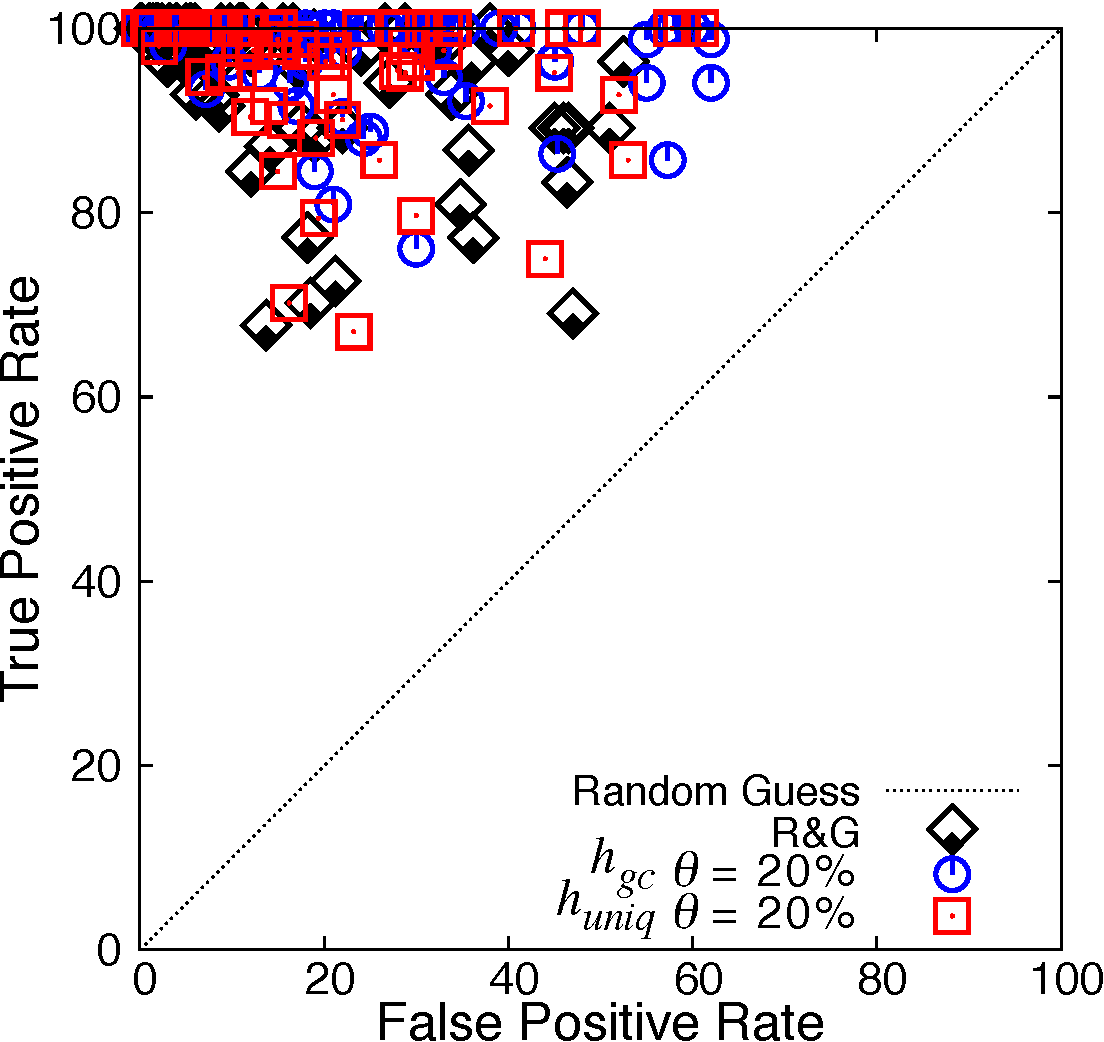
\includegraphics[width=0.6\linewidth]{fig/rocspace-all_domains.pdf}
	\end{figure}
\end{frame}

% @@@@@@@@@@@@@@@@@@@@@@@@@@@@@@@@@@@@@@@@@@@@@@@@@@@@@@@@@@@@@@@	
\begin{frame}{Experiments and Evaluation - Recognition Time}
	\begin{figure}[here]
		\centering
		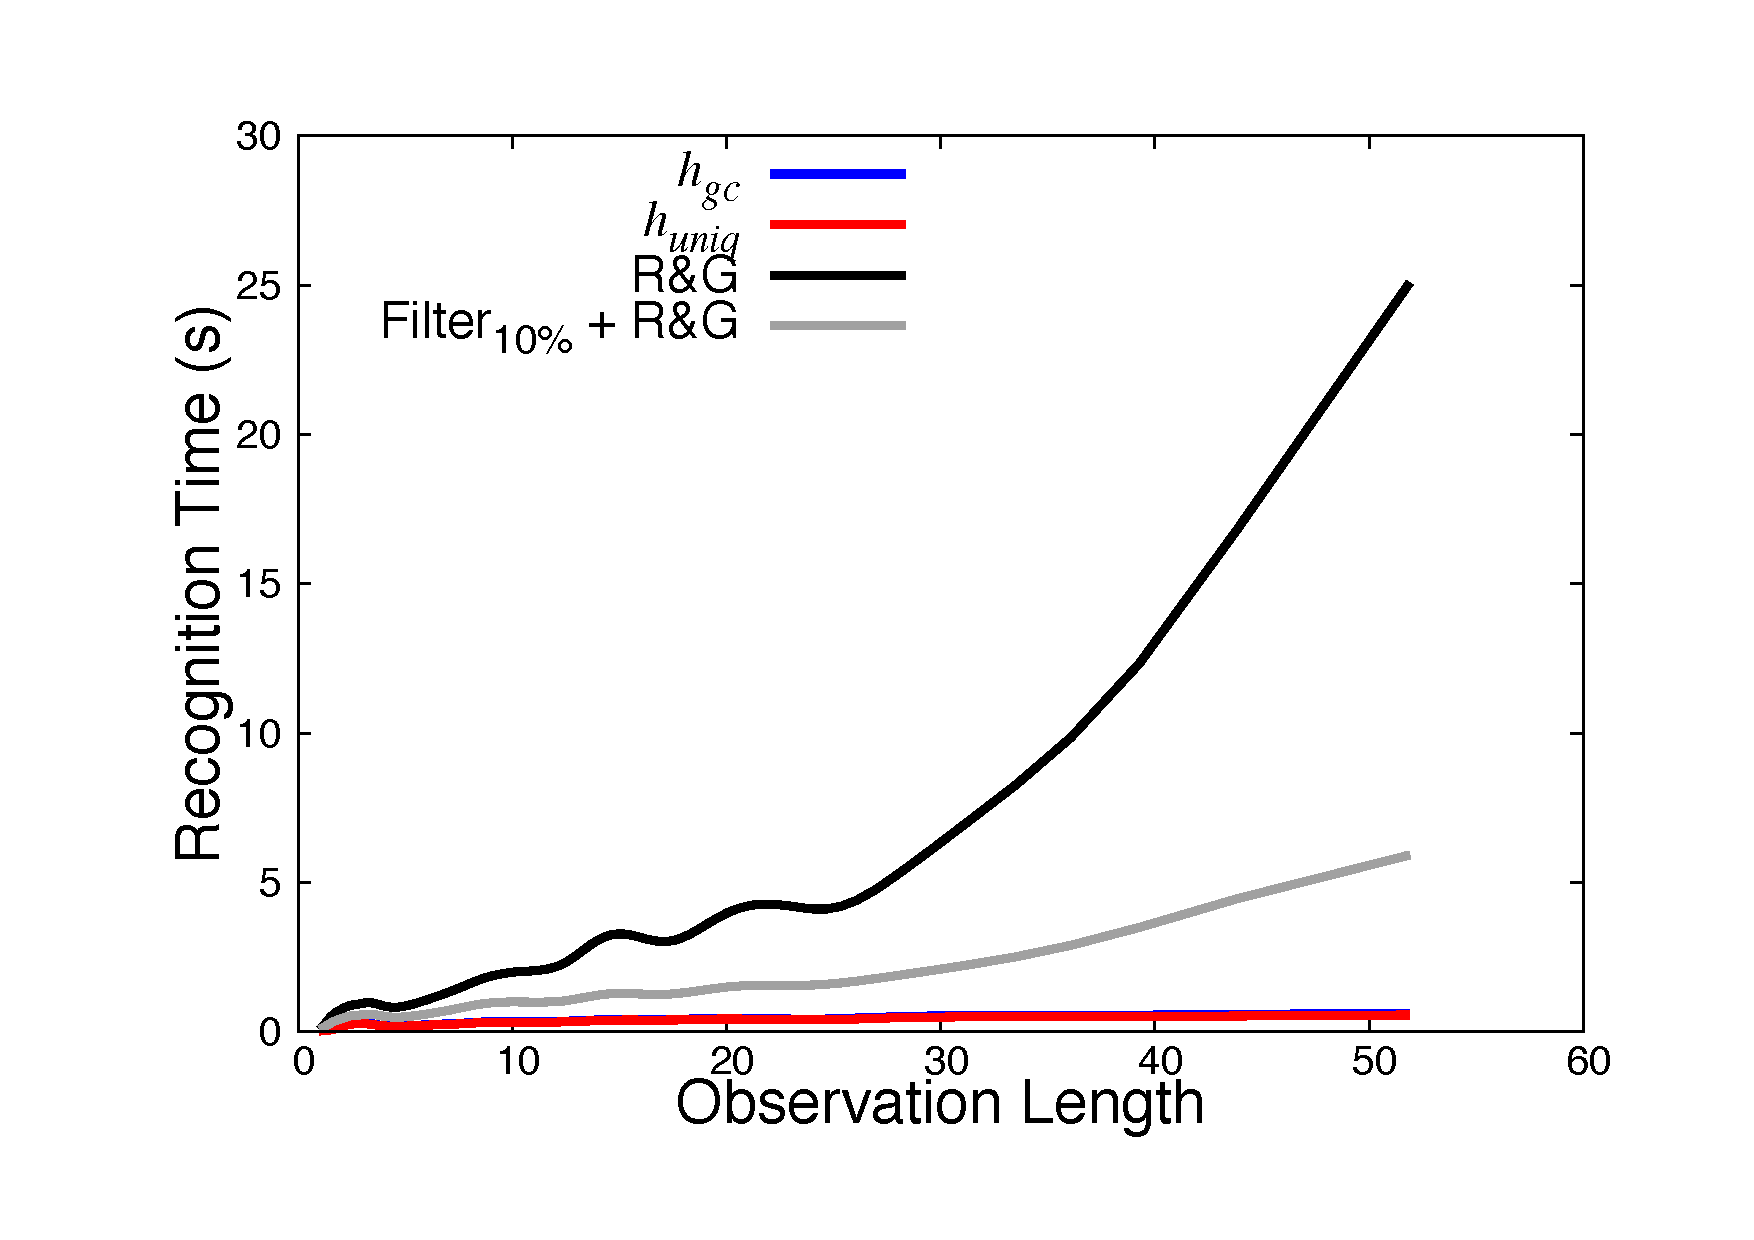
\includegraphics[width=0.7\linewidth]{fig/missing-recognition_time.pdf}
	\end{figure}
\end{frame}

\begin{frame}{Experiments and Evaluation - Recognition Time with Noise}
	\begin{figure}[here]
		\centering
		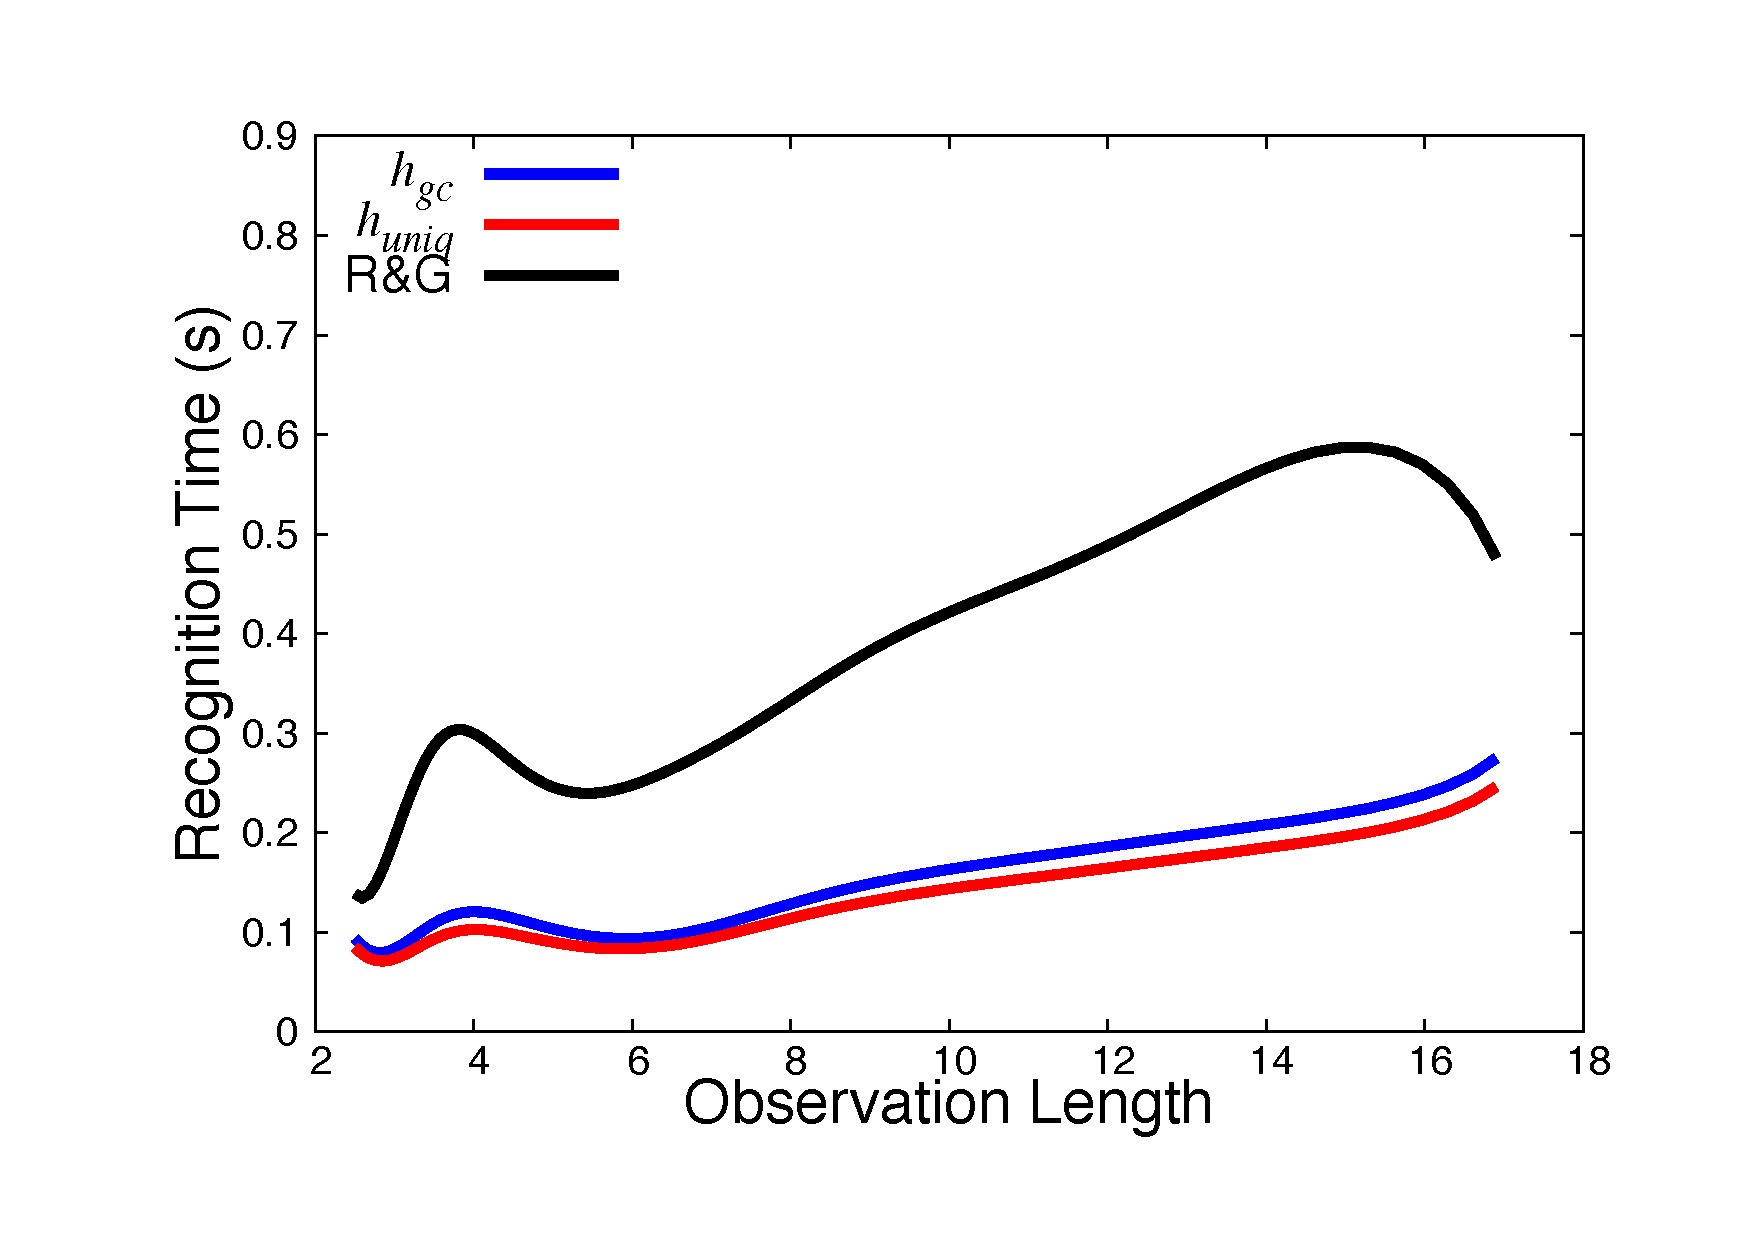
\includegraphics[width=0.7\linewidth]{fig/noisy-recognition_time.pdf}
	\end{figure}
\end{frame}
	
	
%---------------------------------------------------------------------------------
	% RFP - Do we need talk about related work?!
	% \begin{frame}{Related Work}
	% 	\begin{itemize}
	% 		\item ?
	% 	\end{itemize}
	% \end{frame}
	
%---------------------------------------------------------------------------------

\begin{frame}{Contributions and Limitations}
% 	\todo{REDO THIS SLIDE}
   	\begin{itemize}
   		\item \textbf{Contribution so far:}
			\begin{itemize}
				\item Use planning landmarks for goal recognition; 
				\item Obviate the need to run a planner during goal recognition, resulting in much faster and highly accurate recognition; and
                \item Robust dataset to evaluate goal recognition algorithms
			\end{itemize}
		% \item We show that our heuristics are more accurate and much faster than Ramírez and Geffner's approach ({\footnotesize Plan Recognition as Planning. IJCAI, 2009}).
		\item \textbf{Limitations:}
			\begin{itemize}
				\item Sensitive to the presence of landmarks; and
				\item Low accuracy with very few observations, \emph{i.e.}, 10\% of observability;
			\end{itemize}
% 		\item \textbf{Future Work:}
% 			\begin{itemize}
% 				\item Use different landmark extraction algorithms;
% 				\item Use goal ordering techniques; 
% 				\item Derive a probabilistic interpretation for the landmarks; and
% 				\item Apply our landmark-based heuristics to continuous and temporal domains.
% 			\end{itemize}
	\end{itemize}
\end{frame}		

%---------------------------------------------------------------------------------
\section{Online Goal Recognition as Reasoning over Landmarks}

	\begin{frame}[c]\frametitle{Motivation for Efficient Online Goal Recognition}
		Most goal recognition approaches using domain models have three key limitations:
		\begin{enumerate}
			\item assumption of a discrete state-space in a PDDL-like formalism
			\begin{itemize}
				\item not viable for use with path planning scenarios
			\end{itemize}
			\item assume all access to all observations at once
			\begin{itemize}
				\item approaches do not consider the time to recognition
			\end{itemize}
			\item need to call a planner multiple times per goal to rank hypotheses
			\begin{itemize}
				\item PRAP is computationally expensive, impractical for long plans
			\end{itemize}
		\end{enumerate}
	\end{frame}
	
	\begin{frame}[c]\frametitle{Online vs. Offline Plan Recognition}
		\begin{itemize}
			\item Offline plan recognition:
			\begin{itemize}
				\item All observations received at once;
				\item Observations may be incomplete or noisy;
				\item One-shot recognition;
			\end{itemize}
			\item Online plan recognition:
			\begin{itemize}
				\item Observations received incrementally;
                \item Observations may be incomplete or noisy; %(can use facts as observations);
				\item Objective is to recognize goal as soon as possible, without the full observation sequence
			\end{itemize}
		\end{itemize}
		\begin{center}
			\vspace{-3mm}
			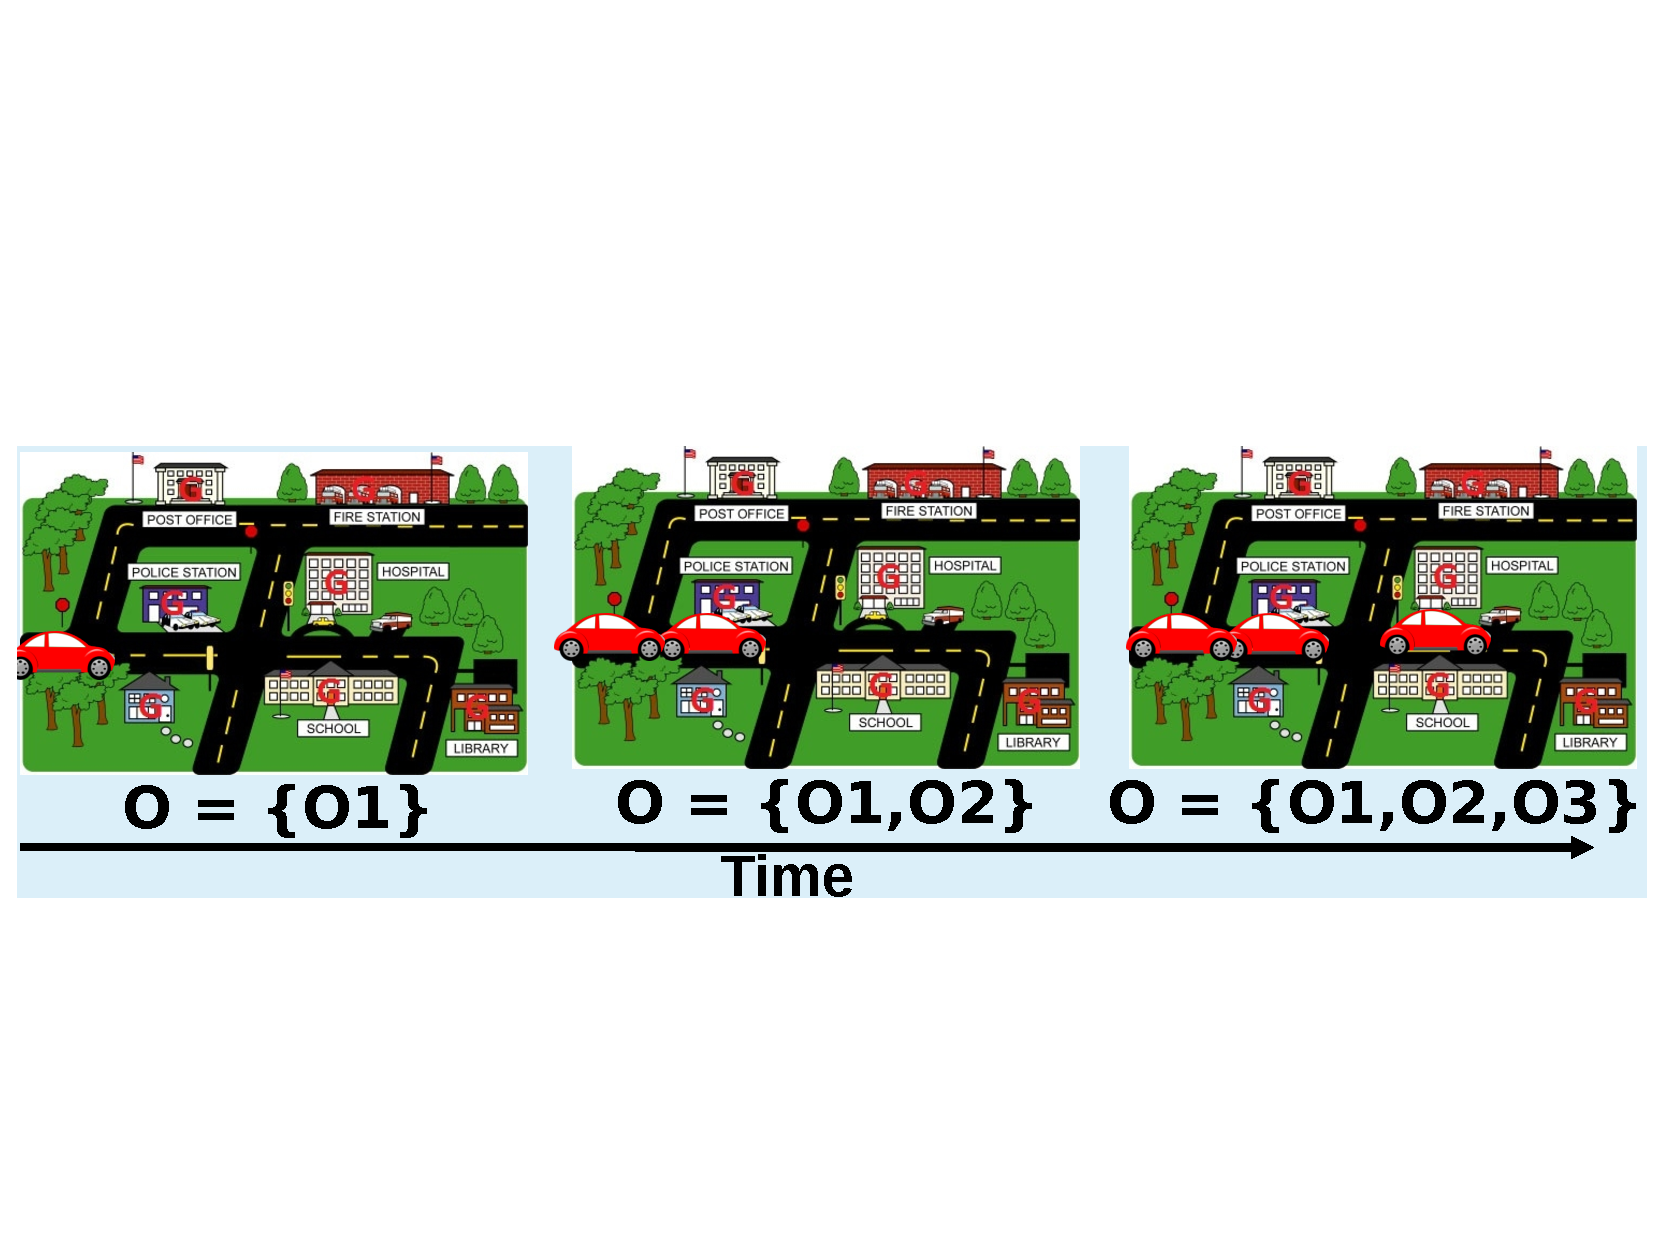
\includegraphics[width=.9\textwidth]{fig/observations-example.pdf}
		\end{center}
	\end{frame}
	
	\begin{frame}[c]\frametitle{Efficient Online Goal Recognition}
		% Thus, want to develop an approach that can:
% 		\begin{itemize}
% 			\item recognize plans over continuous and discrete domains
% 			\item use a full-fledged planner as little as possible
% 			\item return reliable goal ranking as soon as possible
% 		\end{itemize}
		Our approach:
		\begin{itemize}
			\item is efficient for online goal recognition;
			\item works in both discrete and continuous domains;
			\if\masterclass1
			\item uses goal-mirroring to minimize planner calls;
			\else
			\item minimizes planner calls;
			\fi
			\item reasons about landmarks to minimize the number of goal hypotheses; 
			\item returns reliable goal ranking as soon as possible
		\end{itemize}
	\end{frame}
	
\if\masterclass1
	% \begin{frame}[c]\frametitle{Previous Work: Ramirez and Geffner}
% 		\if\masterclass1
% 		\todo{Move this to the background}
% 		\fi
% 		\begin{itemize}
% 			\item First approaches to goal recognition: Plan Recognition as Planning (PRAP)
% 			\item Probabilistic model aims to compute $P(G \mid O)$
% 			\item Following Bayes Rule $P(G \mid O) = \alpha P(O \mid G) P(G)$
% 			\item Given $P(G)$ as a prior, key bottleneck is computing $P(O \mid G)$
% 			\begin{itemize}
% 				\item In their work $P(O \mid G)$ is computed in terms of a cost difference $c(G,O) - c(G,\bar{O})$
% 				\item Computational cost is \textbf{two planner calls per goal hypothesis}
% 				\item For online recognition: two planner calls per goal hypothesis \textbf{per observation}
% 			\end{itemize}
% 			\item Some conclusions challenged for path planning domains\\ (Masters and Sardina 2017)
% 		\end{itemize}
% 	\end{frame}
	
	\begin{frame}[c]\frametitle{Previous Work: Goal Mirroring}
		\begin{itemize}
			\item Focuses on efficient online recognition
			\item Uses a planner to generate plan hypotheses using $(|O|+1)|G|$ planner calls
			\begin{itemize}
				\item Computes optimal plans for each goal
				\item For every incoming observation compute:
				\begin{itemize}
					\item prefix -- concatenation of observations
					\item suffix -- plan from last observation to every goal
				\end{itemize}
				\item Rank plan hypotheses by comparing to ideal plan
			\end{itemize}
		\end{itemize}
	\end{frame}
	
	\begin{frame}[c]\frametitle{Previous Work: Goal Recognition using Heuristics}
		\begin{itemize}
			\item Focuses on efficient recognition with \textbf{no planner calls}
			\item Uses heuristic estimation of states resulting from observation
			\item Ranks goals as a weighed sum based on the number of \textbf{landmarks} visited by the observations
			\item Key characteristics: 
			\begin{itemize}
				\item Very fast (linear on the number of goals and observations)
				\item Less accurate in domains with few landmarks and/or observability
			\end{itemize}
		\end{itemize}
	\end{frame}
\fi
	
	\if\masterclass1
	\begin{frame}[c]\frametitle{Domain formalization}
		The underlying representation adapts from the Transition Normal Form (TNF) (from Pommerening and Helmert), specifically
		\begin{itemize}
			\item Domain model originally dealt with operators that modify the truth-value of \emph{facts} or fluents
			\item We adopt a domain model $M = \langle \mathcal{V}, \mathcal{O} \rangle$:
			\begin{itemize}
				\item $\mathcal{V}$ is a set of variables with a, possibly infinite, domain
				\item operators in $\mathcal{O}$ change the value of all variables in $\mathcal{V}$ from $s$ into $s'$
				\item $cost(o)$ is usually $1$, but when dealing with continuous variables it is the euclidean distance of such values between $s$ and $s'$
			\end{itemize}
		\end{itemize}
	\end{frame}
	
	\begin{frame}[c]\frametitle{Landmarks in Discrete Domains}
		\begin{columns}
			\begin{column}{0.5\textwidth}
				\begin{itemize}
					\item Facts that must be true in all valid plans
					\item Root node is the goal condition
					\item Leaves are facts of initial state
					\item Connected boxes – facts that must be true together
				\end{itemize}
			\end{column}
			\begin{column}{0.5\textwidth}
				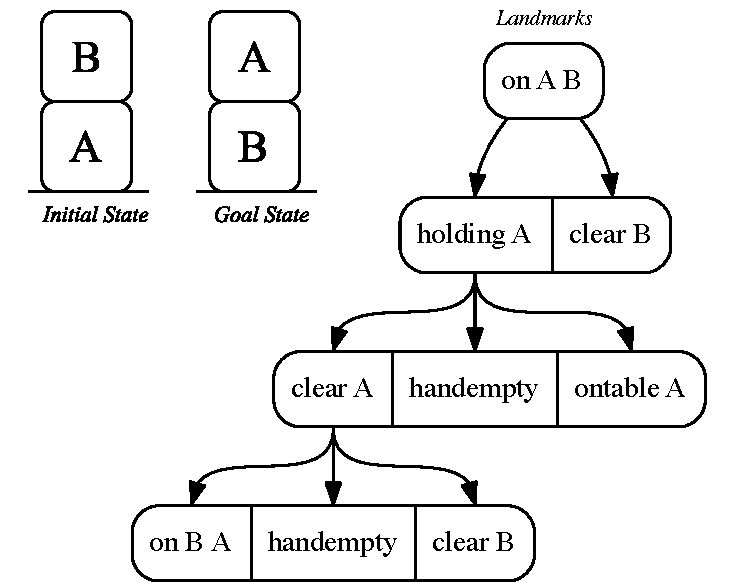
\includegraphics[width=\textwidth]{fig/blocksworld-landmarks-example.pdf}
			\end{column}
		\end{columns}
	\end{frame}
	\fi
	
	\begin{frame}[c]\frametitle{Landmarks in Continuous Domains}
		We need a notion of landmark in continuous domains
		\begin{columns}
			\begin{column}{0.7\textwidth}
			\begin{itemize}
				\item Redefine landmarks as areas surrounding goals
				\begin{itemize}
					\item Goals – Black dots
					\item Surrounding Rectangles – continuous landmark areas
				\end{itemize}
				\item To reach a goal the observed motion must intersect (go through) the corresponding landmark area.
				\item In this work, landmark areas roughly correspond to rooms partitioned as rectangular Voronoi diagrams
				\begin{itemize}
					\item Other notions of numeric landmarks may apply \\(e.g. Scala et al. IJCAI 2017)
				\end{itemize}
			\end{itemize}
			\end{column}
			\begin{column}{0.3\textwidth}
			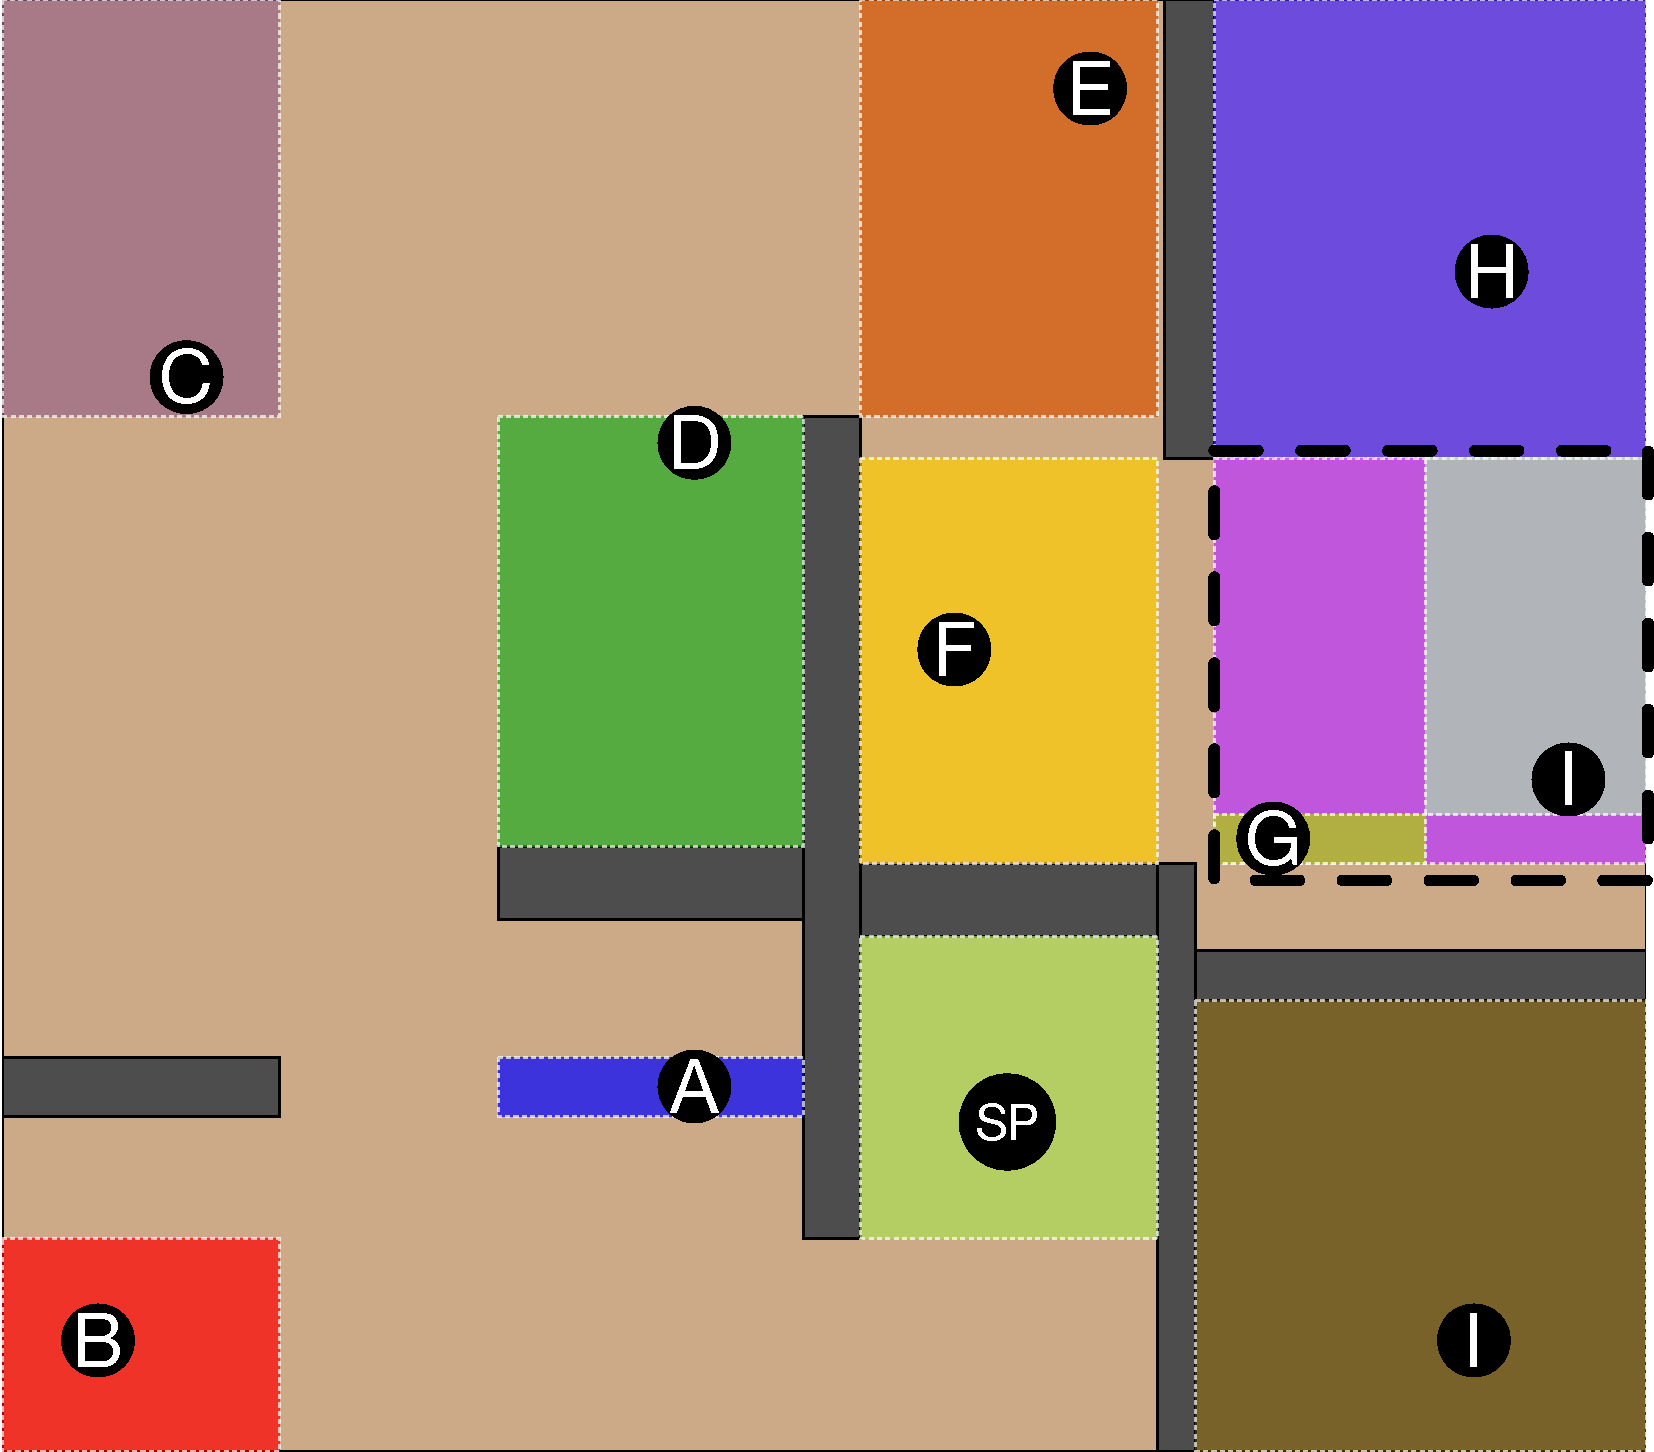
\includegraphics[width=\textwidth]{fig/continuous-landmark-example.pdf}
			\end{column}
		\end{columns}
	\end{frame}
	
	\if\masterclass1
	\begin{frame}[c]\frametitle{Extracting Landmarks in Continuous Domains}
		\begin{columns}
			\begin{column}{0.5\textwidth}
				\onslide<1->{
					1. Partition landmarks using wall aligned squares. \\
				}
				\onslide<2->{
					2. Recursively divide squares with multiple goals using the mid-point in $x,y$ between two randomly selected goals.
				}
			\end{column}
			\begin{column}{0.5\textwidth}
				\only<1>{
					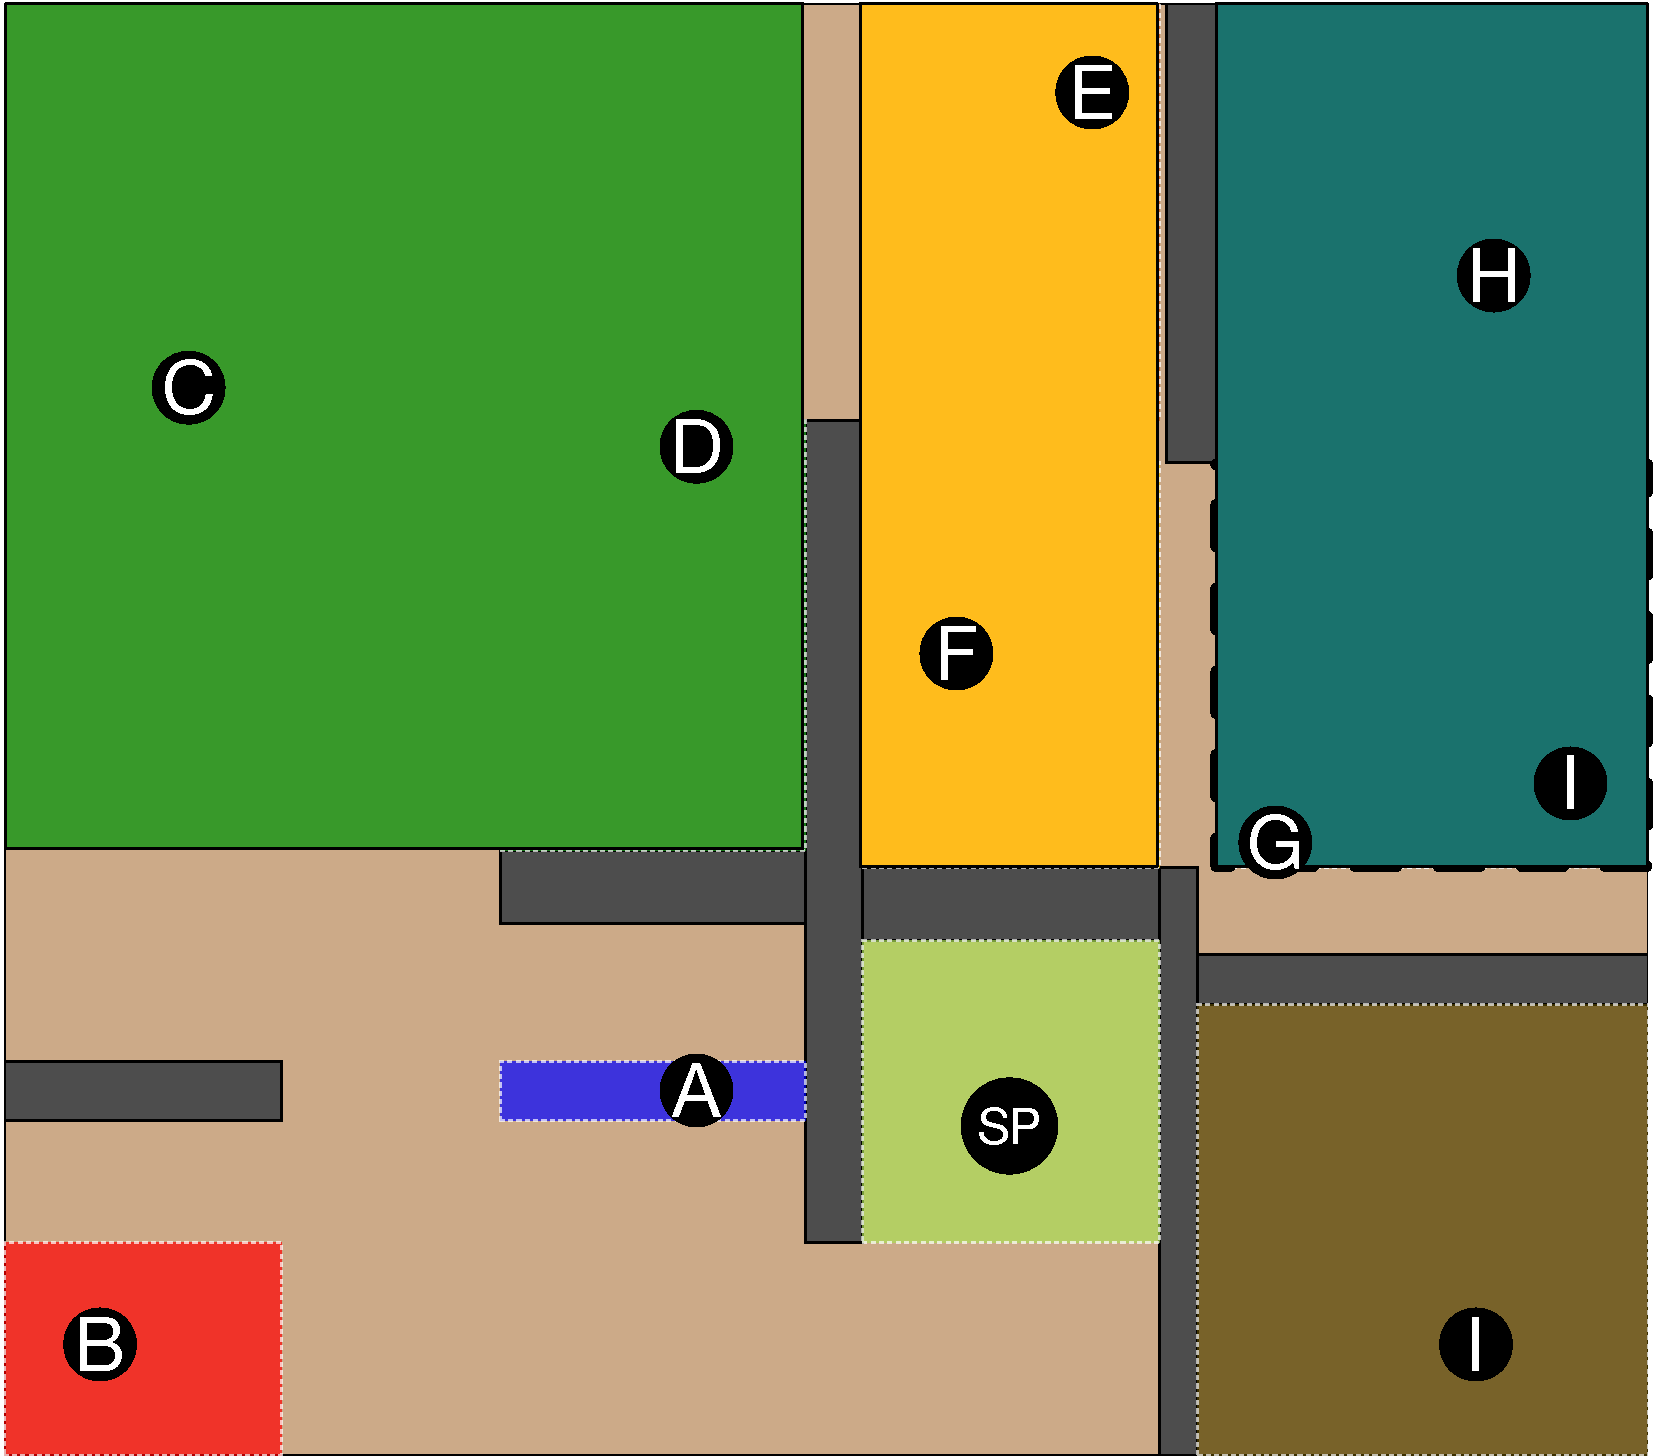
\includegraphics[width=\textwidth]{fig/landmarks-1.pdf}
				}
				\only<2>{
					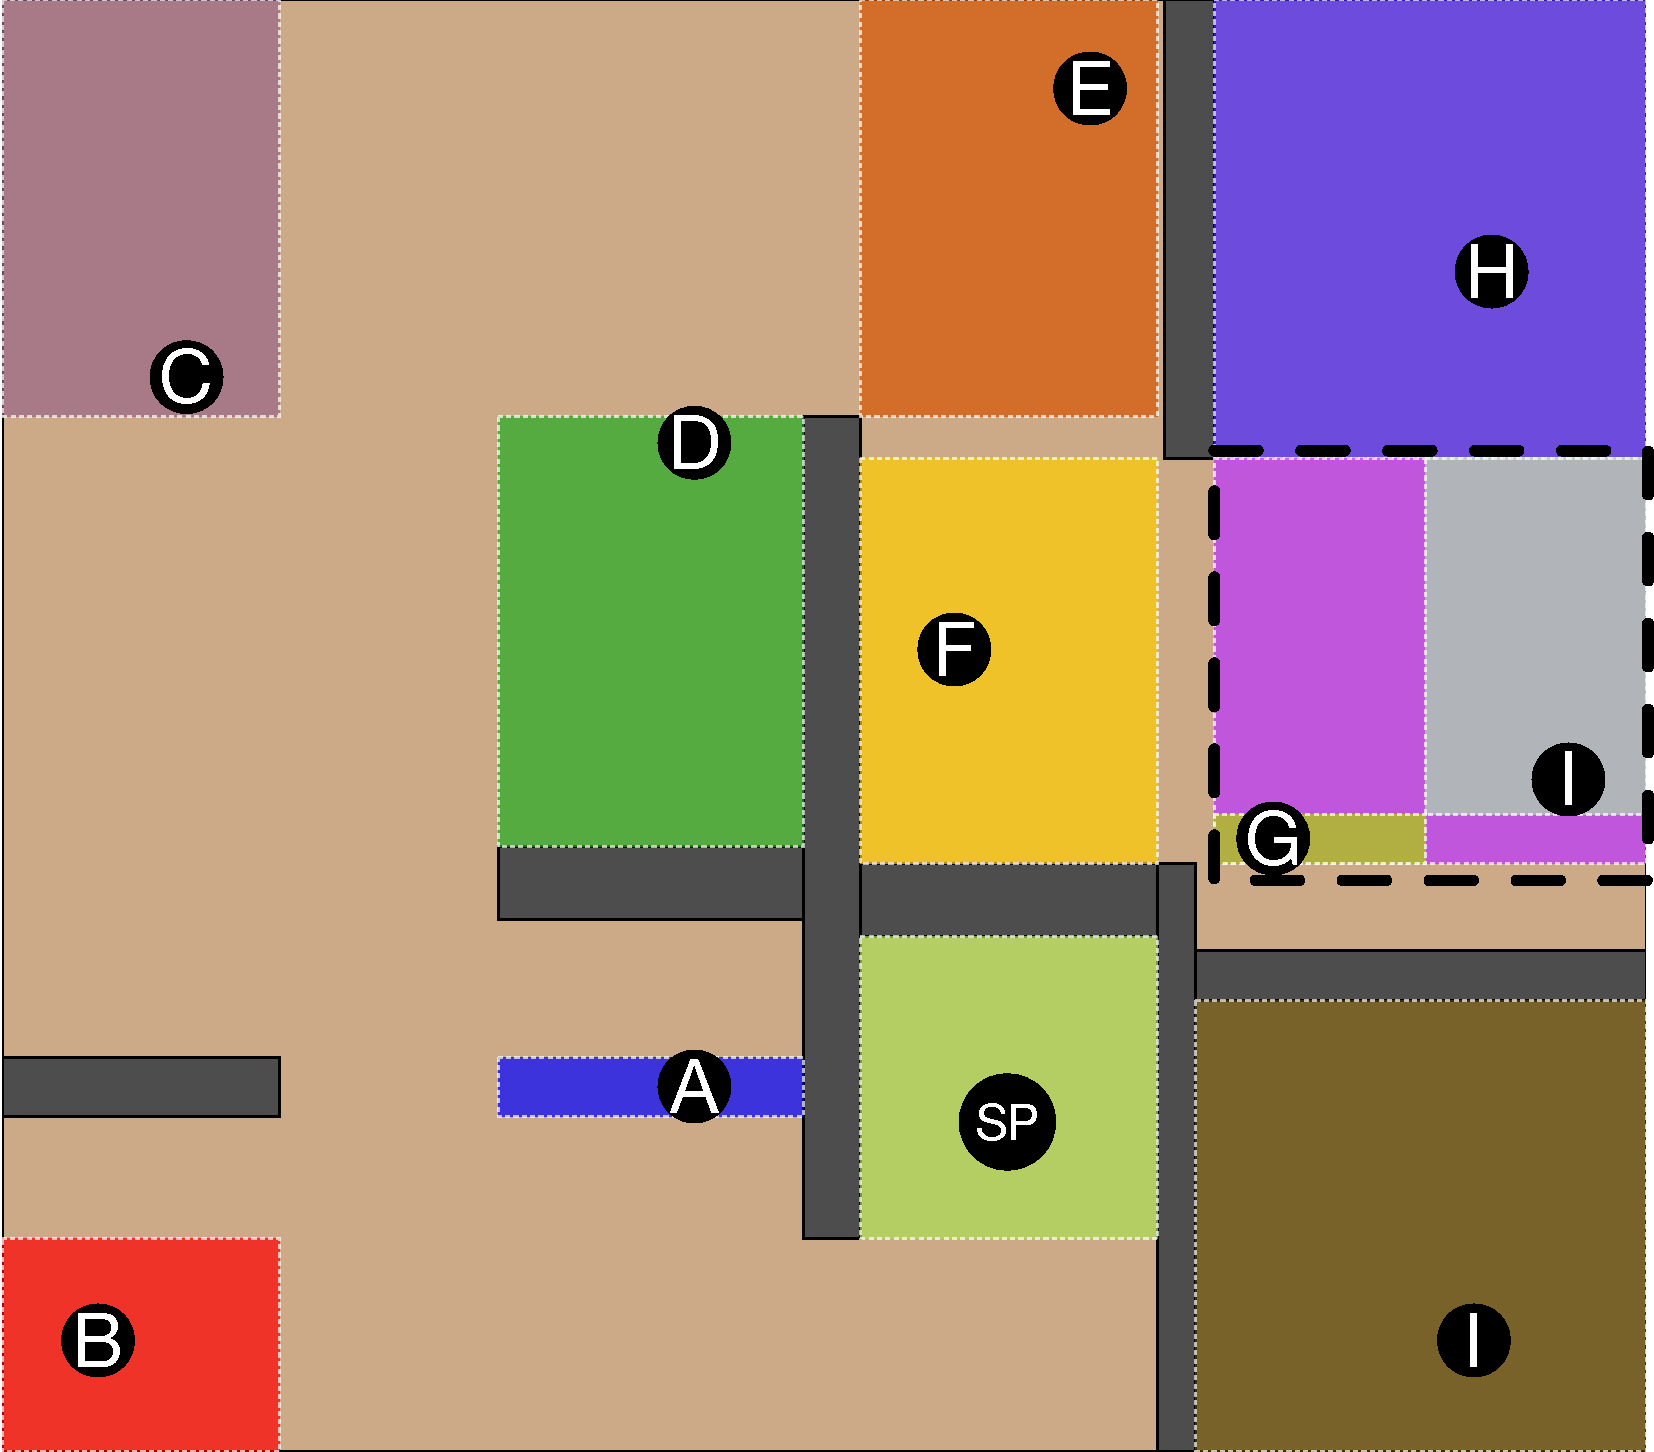
\includegraphics[width=\textwidth]{fig/continuous-landmark-example.pdf}
				}
			\end{column}
		\end{columns}
	\end{frame}
	\fi

	\begin{frame}[c]\frametitle{Online Recognition with Landmarks}
		\begin{columns}
			\begin{column}{0.7\textwidth}
			\begin{itemize}
				\item Generate the ordered set of achieved landmarks
				\item Maintain the group of goals eliminated due to landmarks
				\item For every observation:
				\begin{itemize}
					% \item Check if it caused any landmarks to be achieved
					\item Check if it ``achieved'' a landmark
					% \item Intersect observation point with landmark areas
					\item If observations backtrack, re-instate goals
				\end{itemize}
				\item Rank goals using the landmark completion heuristic $h_{gc}$
			\end{itemize}
			\end{column}
			\begin{column}{0.3\textwidth}
				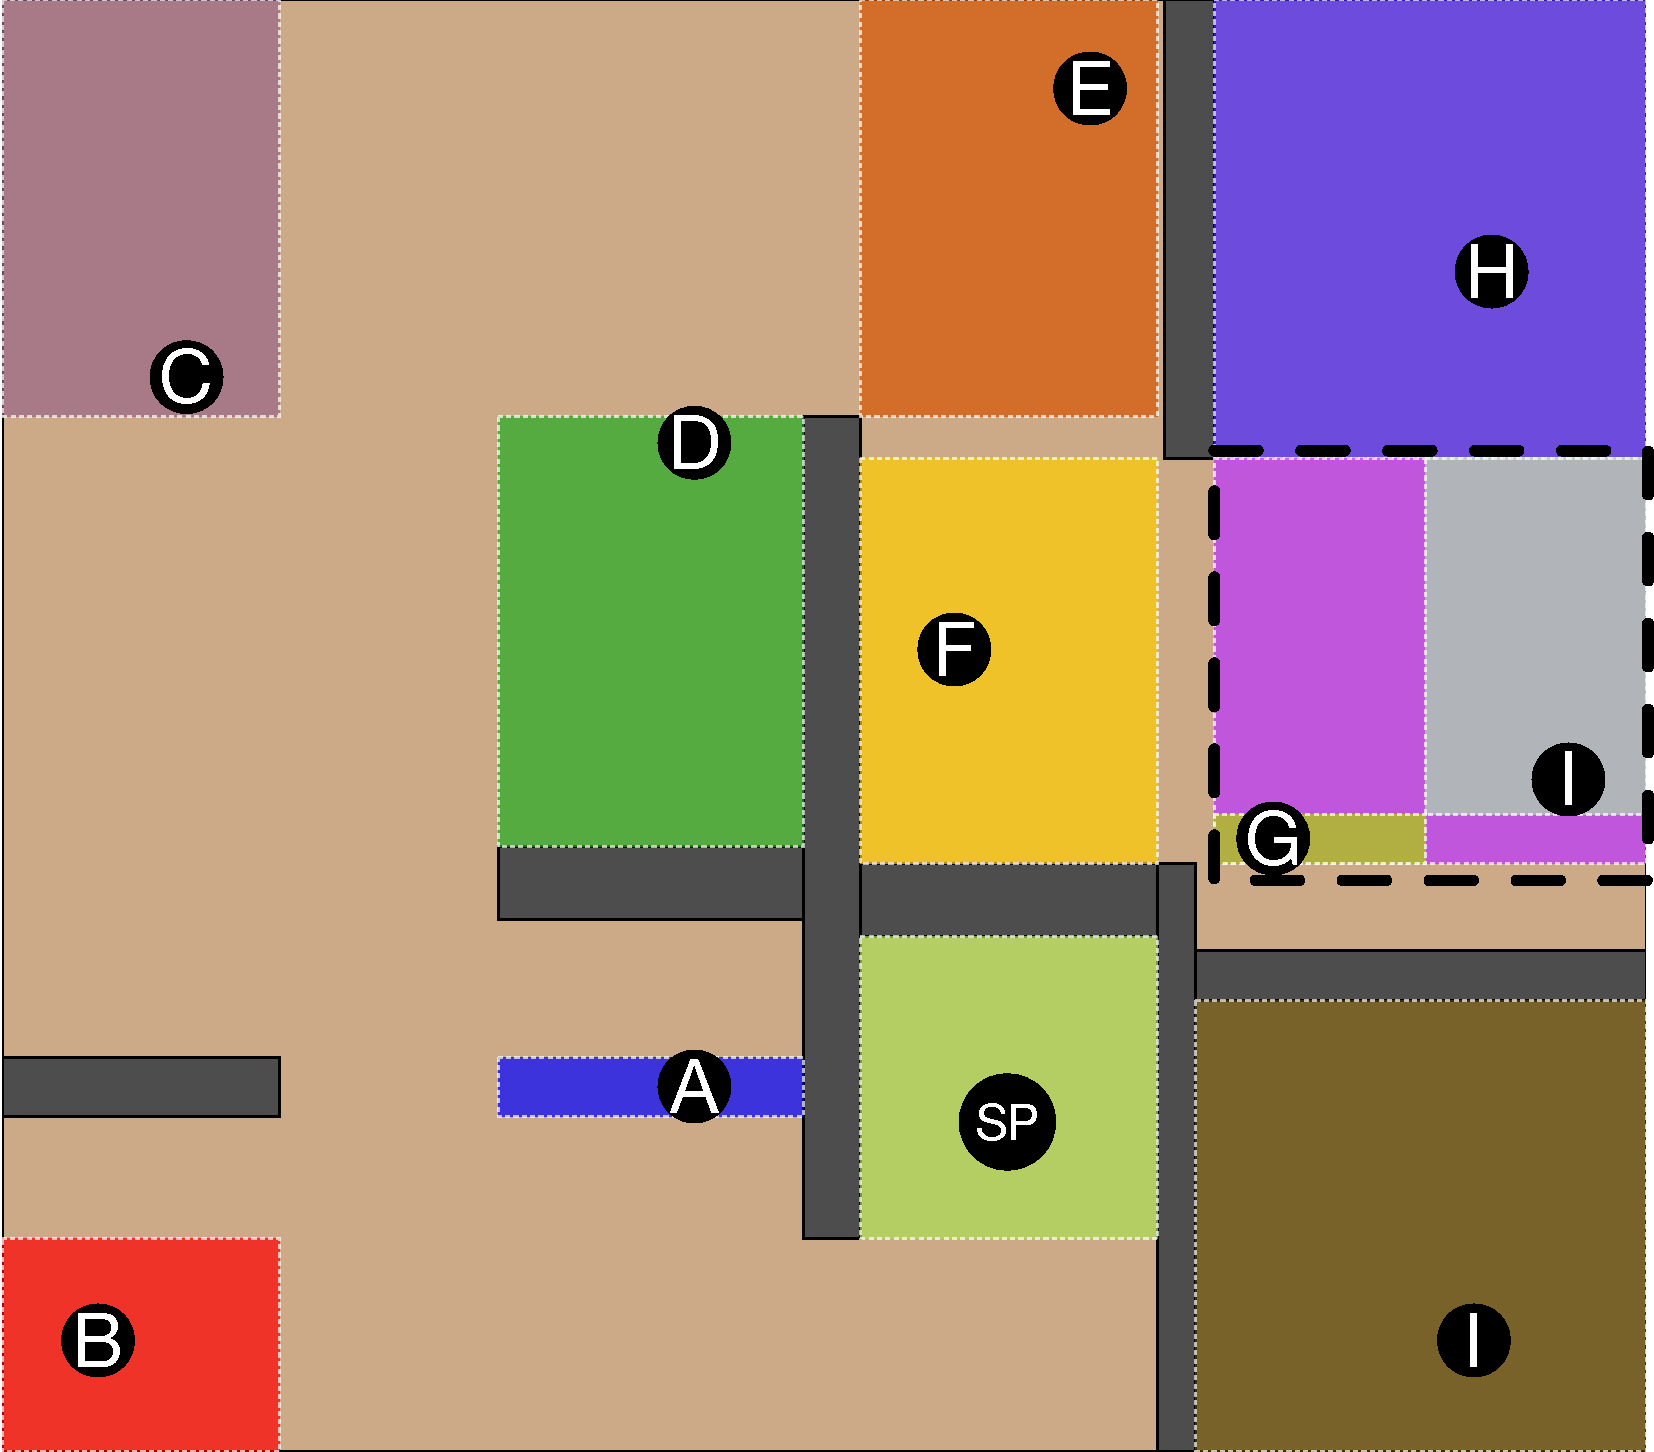
\includegraphics[width=\textwidth]{fig/continuous-landmark-example.pdf}
			\end{column}
		\end{columns}
	\end{frame}
	
	% \if\masterclass1
% 	\begin{frame}[c]\frametitle{Online Recognition with Landmarks}
% 		\todo{For masterclass, put algorithm with example}
% 	\end{frame}
% 	\fi
	
	\begin{frame}[c]\frametitle{Goal Mirroring with Landmarks}
		Combines landmark reasoning with goal mirroring
		\begin{columns}
			\begin{column}{0.7\textwidth}
			\begin{itemize}
				\item Compute landmarks and optimal plans for all goals
				\item For every observation:
				\begin{itemize}
					\item Compute plan prefix, and for every goal
					\begin{itemize}
						\item Either prune goals that have \textbf{passed} the last landmark; or
						\item Compute plan suffix (from last observation) using planner
						\item Compute \textbf{cost ratio} between prefix+suffix and optimal plan
					\end{itemize}
				\end{itemize}
				\item Rank unpruned goals based on a \textbf{normalized cost ratio}
			\end{itemize}
			\end{column}
			\begin{column}{0.3\textwidth}
				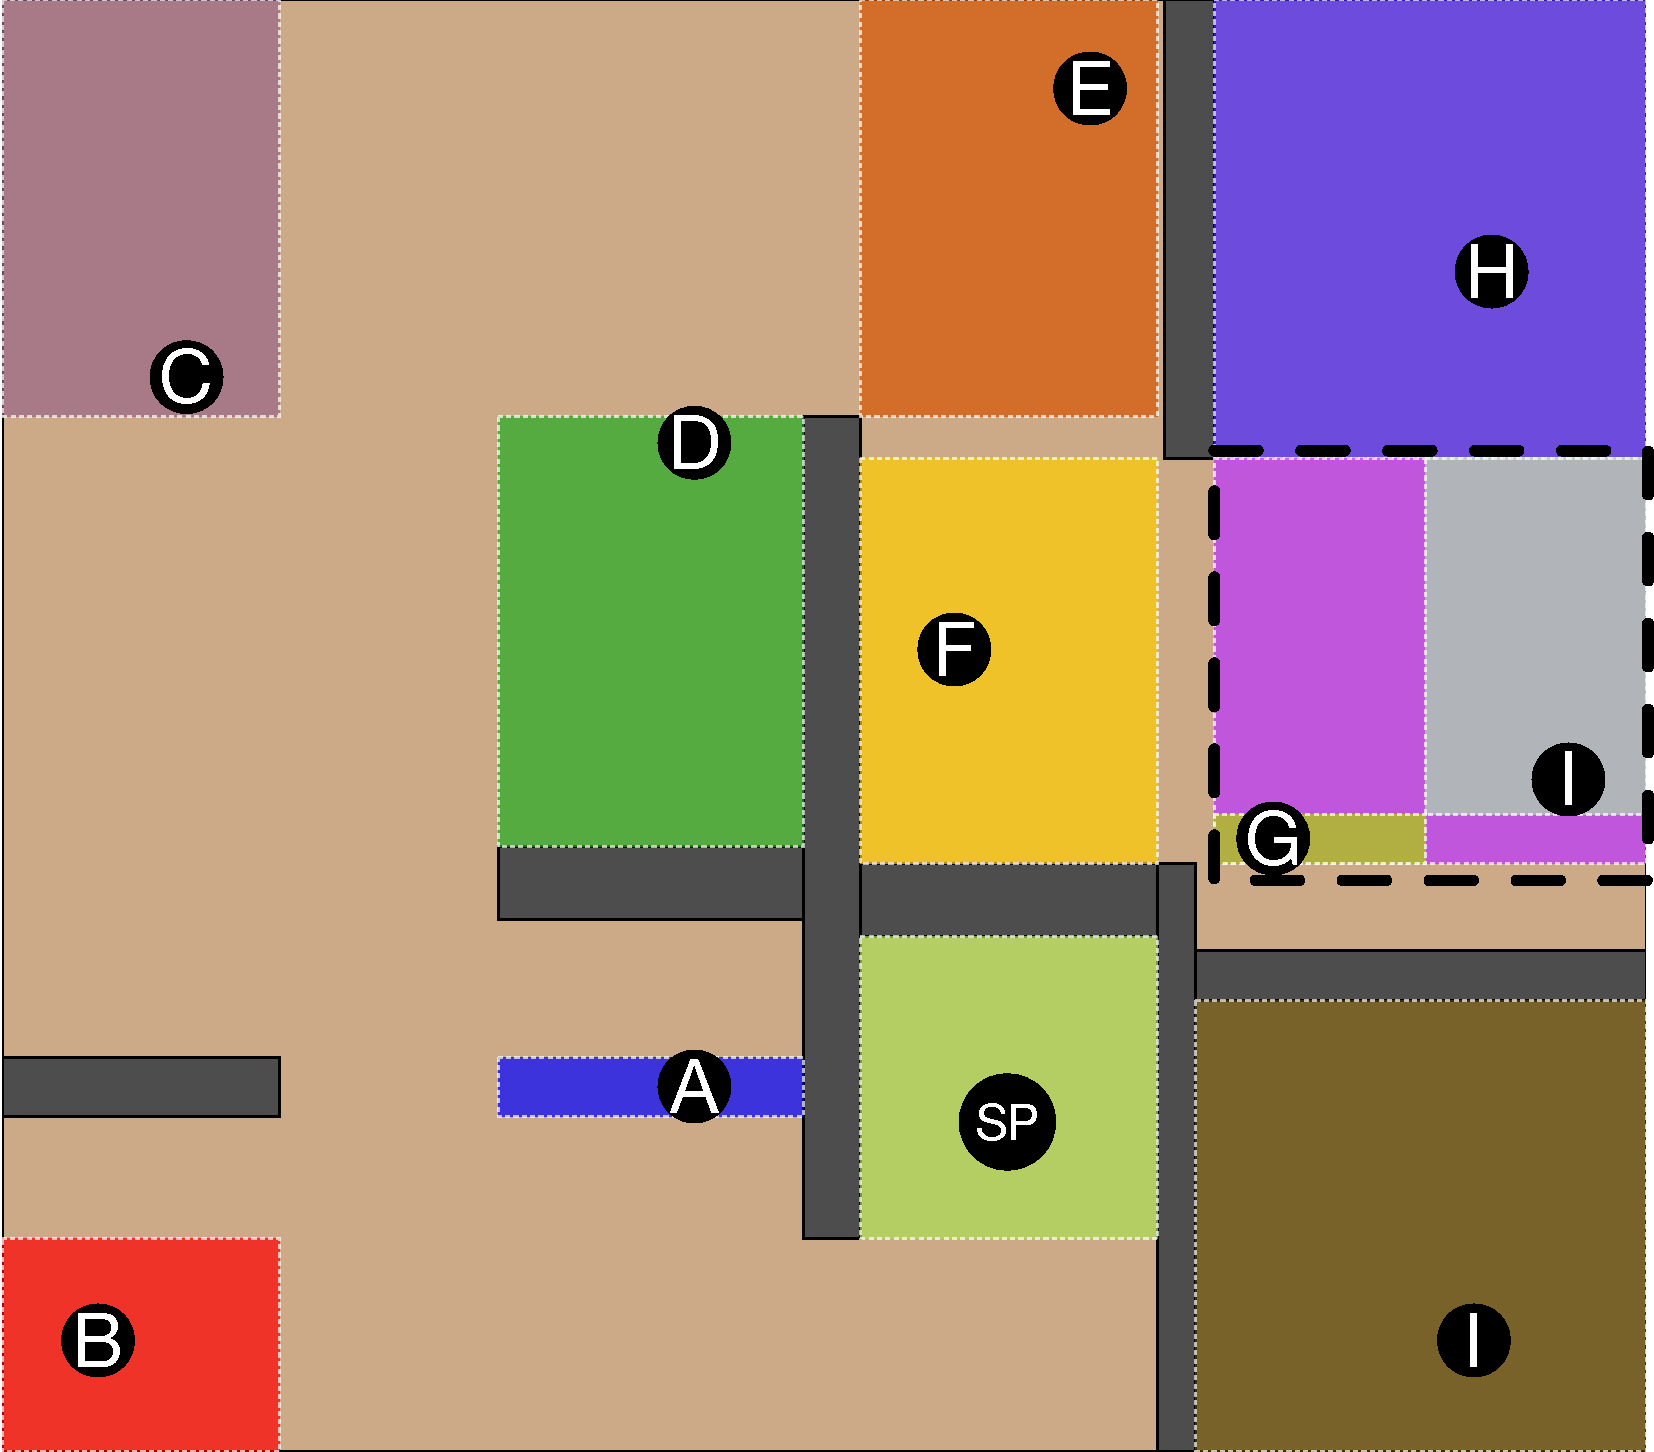
\includegraphics[width=\textwidth]{fig/continuous-landmark-example.pdf}
			\end{column}
		\end{columns}
		\begin{itemize}
			\item Ranks $P(g_k \mid O)$ using a normalizing factor $\eta 1/\sum_{g_k \in G} rank(g_k)$
			\item Approximates $P(g \mid O) = \eta \sum_{g_k \in G} P(O \mid g_k) P(g_k)$ for all goals, assuming $P(g_k) = 0$ for pruned goals 
		\end{itemize}
	\end{frame}
	
	\if\masterclass1
	\begin{frame}[c]\frametitle{Goal Mirroring with Landmarks}
		\todo{Algorithm and example for masterclass}
	\end{frame}
	\fi
	
	\begin{frame}[c]\frametitle{Continuous Evaluation}
		\begin{columns}
			\begin{column}{0.7\textwidth}
				\begin{itemize}
					\item Cubicles environment and robot (OMPL)
					\item 11 points spread evenly over the environment
					%\item Two different paths from start to goal 110*2 problems
					\item 220 problems
				\end{itemize}
		\end{column}
		\begin{column}{0.3\textwidth}
			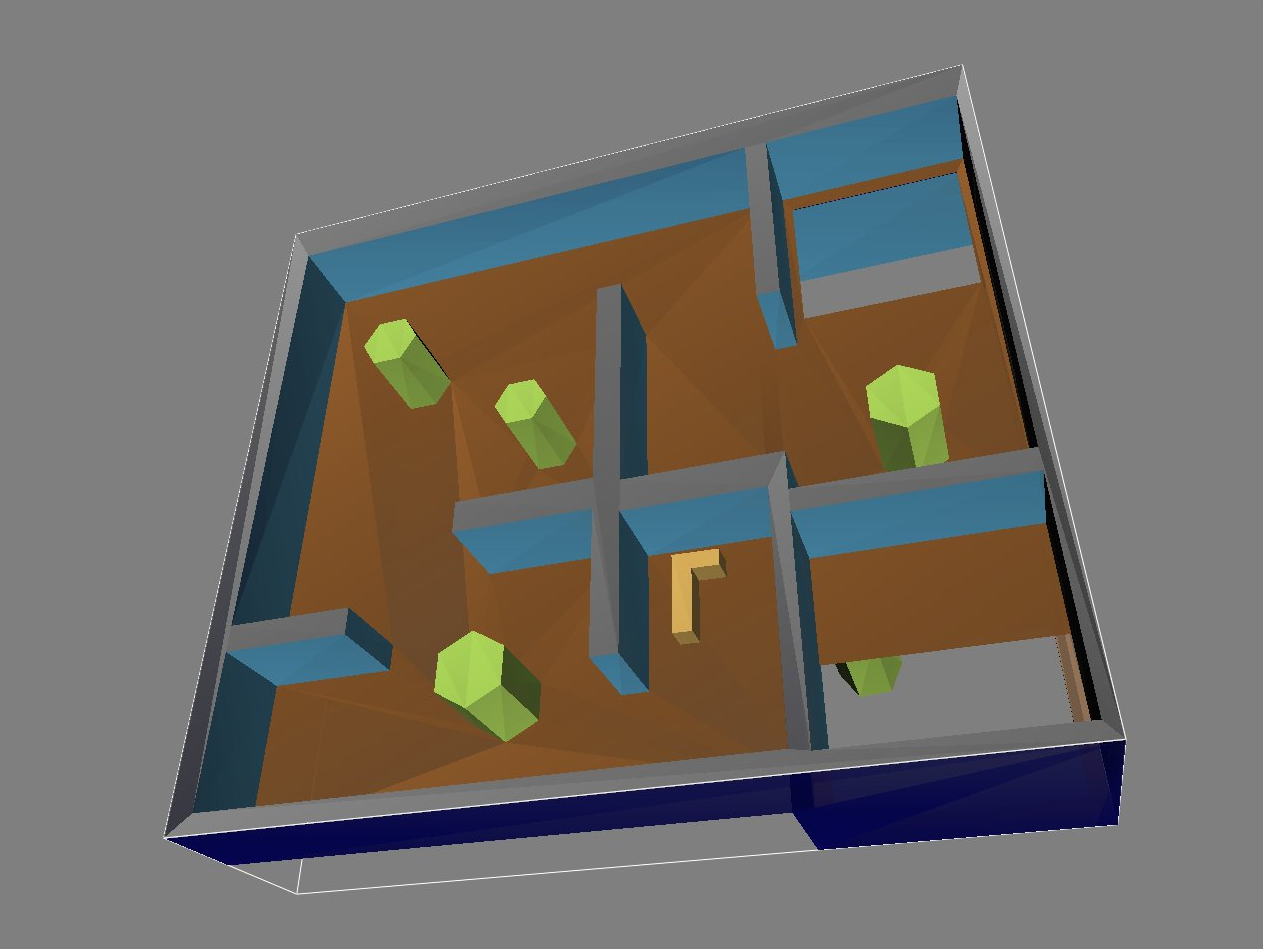
\includegraphics[width=\textwidth]{fig/CubiclesEnv_RobotOnlyView.png}
		\end{column}
		\end{columns}
	\end{frame}

% \if\masterclass1
	\begin{frame}[c]\frametitle{Discrete Evaluation}
		\begin{columns}
			\begin{column}{0.7\textwidth}
				\begin{itemize}
					\item Dataset expanded from Ramirez and Geffner's original work
					\item Domains extracted from the IPC competition
					\item Hundreds of goal recognition problems
				\end{itemize}
			\end{column}
			\begin{column}{0.3\textwidth}
			Domains
			\begin{itemize}
				\tiny
				\item \textsc{Blocks-World}
				\item \textsc{Campus}
				\item \textsc{Depots}
				\item \textsc{Driver-Log}
				\item \textsc{Dock-Worker-Robots}
				\item \textsc{Easy-IPC-Grid}
				\item \textsc{Ferry}
				\item \textsc{Intrusion-Detection}
				\item \textsc{Kitchen}
				\item \textsc{Logistics}
				\item \textsc{Miconic}
				\item \textsc{Rovers}
				\item \textsc{Satellite}
				\item \textsc{Sokoban}; and
				\item \textsc{Zeno-Travel}
			\end{itemize}
			\end{column}
		\end{columns}
	\end{frame}
% \fi

% \if\masterclass1
% 	\begin{frame}[c]\frametitle{Performance Results}
% 		\todo{Redo this table for the masterclass}
% 		\newcommand{\timeout}{\fontsize{4}{4}\selectfont \textit{Timeout}}
% 		\tiny
% 		\begin{tabular}{llll|cccccc|cccccc|cccccc|}
% 		\cline{5-22}
% 		                                                                                              &                                &                                &               & \multicolumn{18}{c|}{\bf Continuous Domains}                                                                                                                                      \\ \cline{5-22}
% 		                                                                                              &                                &                                &               & \multicolumn{6}{c|}{\sc Goal Mirroring}
% 		& \multicolumn{6}{c|}{\sc Goal Mirroring with Landmarks}
% 		& \multicolumn{6}{c|}{\sc Online Recognition with Landmarks}                                                            \\ \hline
% 		\multicolumn{1}{|c|}{\textit{\begin{tabular}[c]{@{}c@{}}Domain\\ (\# problems)\end{tabular}}\hspace{0.2em}}
% 		& \multicolumn{1}{c}{\textit{$|G|$}} & \multicolumn{1}{c}{\textit{$|O|$}} & \multicolumn{1}{c|}{\textit{$|L|$}}
% 		& \textit{Time}     & \textit{PC} & \textit{TPR} & \textit{FPR} & \textit{RF} & \textit{CV}
% 		& \textit{Time}     & \textit{PC} & \textit{TPR} & \textit{FPR} & \textit{RF} & \textit{CV}
% 		& \textit{Time}     & \textit{PC} & \textit{TPR} & \textit{FPR} & \textit{RF} & \textit{CV} \\ \hline
%
% 		\multicolumn{1}{|c|}{\begin{tabular}[c]{@{}c@{}}Cubicles\\ (220)\end{tabular}\hspace{0.2em}}
% 			& \multicolumn{1}{c}{11.0}
% 			& \multicolumn{1}{c}{26.5}
% 			& \multicolumn{1}{c|}{11.0}
% 			% Mirroring Results
% 			& 104.70	& 265.0		& \textbf{100\%}		& 100\%		& 20.2\%	& 21.8\%
%
% 			% Mirroring with Landmarks
% 			& 85.90 	& 184.8		& 78.2\%	& 61.1\%	& \textbf{24.3\%}	& \textbf{26.2\%}
%
% 			% Landmarks
% 			& \textbf{0.020}  & \textbf{0}	& 78.3\%	& \textbf{60.9\%}	& 21.7\%	&	15\% \hspace{0.3em}             \\ \hline
% 		\end{tabular}
%
% 		\vspace{1mm}
%
% 		\begin{tabular}{llll|cccccc|cccccc|cccccc|}
% 		\cline{5-22}
% 		                                                                                              &                                &                                &               & \multicolumn{18}{c|}{\bf Discrete Domains}                                                                                                                                      \\ \cline{5-22}
% 		                                                                                              &                                &                                &               & \multicolumn{6}{c|}{\sc Goal Mirroring}
% 		& \multicolumn{6}{c|}{\sc Goal Mirroring with Landmarks}
% 		& \multicolumn{6}{c|}{\sc Online Recognition with Landmarks}                                                            \\ \hline
% 		\multicolumn{1}{|c|}{\textit{\begin{tabular}[c]{@{}c@{}}Domain\\ (\# problems)\end{tabular}}}
% 		& \multicolumn{1}{c}{\textit{$|G|$}} & \multicolumn{1}{c}{\textit{$|O|$}} & \multicolumn{1}{c|}{\textit{$|L|$}}
% 		& \textit{Time}     & \textit{PC} & \textit{TPR} & \textit{FPR} & \textit{RF} & \textit{CV}
% 		& \textit{Time}     & \textit{PC} & \textit{TPR} & \textit{FPR} & \textit{RF} & \textit{CV}
% 		& \textit{Time}     & \textit{PC} & \textit{TPR} & \textit{FPR} & \textit{RF} & \textit{CV} \\ \hline
%
% 		\multicolumn{1}{|c|}{\begin{tabular}[c]{@{}c@{}}Campus\\ (15)\end{tabular}}
% 			& \multicolumn{1}{c}{2.0}
% 			& \multicolumn{1}{c}{5.4}
% 			& \multicolumn{1}{c|}{8.6}
% 			% Mirroring Results
% 			& 0.441		& 12.8	& 60.0\%	& 21.3\% 	& 57.3\% 	& 41.3\%
%
% 			% Mirroring with Landmarks
% 			& 0.212		& 7.7	& \textbf{96.4\%}	& \textbf{1.7\%}	& \textbf{96.4\%} 	& \textbf{96.4\%}
%
% 			% Landmarks
% 			& \textbf{0.065} & \textbf{0}	& 92.8\%	& 3.5\%		& 92.8\% 	& 92.8\%              \\ \hline
%
% 		\multicolumn{1}{|c|}{\begin{tabular}[c]{@{}c@{}}IPC-Grid\\ (61)\end{tabular}}
% 			& \multicolumn{1}{c}{8.3}
% 			& \multicolumn{1}{c}{21.8}
% 			& \multicolumn{1}{c|}{10.2}
% 			% Mirroring Results
% 			& 10.36		& 209.1		& \textbf{87.2\%}	& 19.4\%	& 36.6\% 	& 35.6\%
%
% 			% Mirroring with Landmarks
% 			& 3.29		& 71.2		& 55.6\%	& \textbf{10.5\%} 	& \textbf{45.8\%}	& \textbf{41.5\%}
%
% 			% Landmarks
% 			& \textbf{0.335}	& \textbf{0}	& 59.4\%	& 21.8\% 	& 32.6\%	& 31.1\%              \\ \hline
%
% 		\multicolumn{1}{|c|}{\begin{tabular}[c]{@{}c@{}}Ferry\\ (28)\end{tabular}}
% 			& \multicolumn{1}{c}{7.5}
% 			& \multicolumn{1}{c}{24.2}
% 			& \multicolumn{1}{c|}{28.5}
% 			% Mirroring Results
% 			& 55.24	& 179.5		& 83.1\%	& 10.2\% 	& 59.2\%	& 57.2\%
%
% 			% Mirroring with Landmarks
% 			& 7.98	& 35.4		& \textbf{83.3\%}	& \textbf{3.1\%} 	& \textbf{82.4\%}	& \textbf{82.1\%}
%
% 			% Landmarks
% 			& \textbf{0.101}	& \textbf{0}		& 82.4\%	& 5.4\%  & 72.5\%	& 71.9\%              \\ \hline
%
% 		\multicolumn{1}{|c|}{\begin{tabular}[c]{@{}c@{}}Intrusion\\ (45)\end{tabular}}
% 			& \multicolumn{1}{c}{16.6}
% 			& \multicolumn{1}{c}{13.1}
% 			& \multicolumn{1}{c|}{16.0}
% 			% Mirroring Results
% 			& 2.02	& 235.5		& \textbf{100\%}		& 7.2\% 	& 55.3\%	& 55.3\%
%
% 			% Mirroring with Landmarks
% 			& 0.257	& 34.7		& 75.5\%	& \textbf{3.6\%} 	& \textbf{67.1\%}	& \textbf{67.1\%}
%
% 			% Landmarks
% 			& \textbf{0.127}	& \textbf{0}	& 87.6\%	& 3.9\% 	& 57.1\%	& 55.1\%              \\ \hline
%
% 		\multicolumn{1}{|c|}{\begin{tabular}[c]{@{}c@{}}Kitchen\\ (15)\end{tabular}}
% 			& \multicolumn{1}{c}{3.0}
% 			& \multicolumn{1}{c}{7.4}
% 			& \multicolumn{1}{c|}{5.0}
% 			% Mirroring Results
% 			& 0.141	& 25.4		& 70.1\%	& 18.4\% 	& 44.6\%	& 36.1\%
%
% 			% Mirroring with Landmarks
% 			& 0.07	& 20.0		& 77.6\%	& \textbf{17.9\%} 	& \textbf{62.6\%}	& \textbf{58.3\%}
%
% 			% Landmarks
% 			& \textbf{0.04}	& \textbf{0}	& \textbf{100\%}		& 50\% 		& 23.9\%	& 23.9\%              \\ \hline
%
% 		\multicolumn{1}{|c|}{\begin{tabular}[c]{@{}c@{}}Logistics\\ (61)\end{tabular}}
% 			& \multicolumn{1}{c}{10.4}
% 			& \multicolumn{1}{c}{24.4}
% 			& \multicolumn{1}{c|}{16.1}
% 			% Mirroring Results
% 			& 53.82	& 199.3		& \textbf{95.4\%}	& 14.7\% 	& 26.9\%	& 25.8\%
%
% 			% Mirroring with Landmarks
% 			& 14.39	& 49.6		& 61.7\%	& \textbf{6.7\%} 	& \textbf{49.1\%}	& \textbf{48.4\%}
%
% 			% Landmarks
% 			& \textbf{0.594}	& \textbf{0}	& 56.1\%	& 9.5\% 	& 40.5\%	& 40.5\%              \\ \hline
%
% 		\multicolumn{1}{|c|}{\begin{tabular}[c]{@{}c@{}}Rovers\\ (28)\end{tabular}}
% 			& \multicolumn{1}{c}{6.0}
% 			& \multicolumn{1}{c}{24.9}
% 			& \multicolumn{1}{c|}{19.8}
% 			% Mirroring Results
% 			& \timeout	& -	& -	& -	& - & -
%
% 			% Mirroring with Landmarks
% 			& 58.87	& 31.1		& \textbf{76.8\%}	& \textbf{4.8\%} 	& \textbf{76.2\%}	& \textbf{75.1\%}
%
% 			% Landmarks
% 			& \textbf{0.867}	& \textbf{0}	& 72.1\%	& 8.5\% 	& 62.1\%	& 62.1\%              \\ \hline
%
% 		\multicolumn{1}{|c|}{\begin{tabular}[c]{@{}c@{}}Satellite\\ (28)\end{tabular}}
% 			& \multicolumn{1}{c}{6.4}
% 			& \multicolumn{1}{c}{16.9}
% 			& \multicolumn{1}{c|}{10.1}
% 			% Mirroring Results
% 			& 93.89	& 177.2		& \textbf{100\%}		& 33.8\% 	& 36.1\%	& 36.1\%
%
% 			% Mirroring with Landmarks
% 			& 5.18	& 30.6		& 81.8\%	& 9.4\% 	& \textbf{72.8\%}	& \textbf{71.9\%}
%
% 			% Landmarks
% 			& \textbf{1.09}	& \textbf{0}	& 78.2\%	& \textbf{9.3\%} 	& 64.4\%	& 64.1\%              \\ \hline
% 		\end{tabular}
% 	\end{frame}
% \fi
	
	\begin{frame}[c]\frametitle{Performance Results}
		\begin{center}
			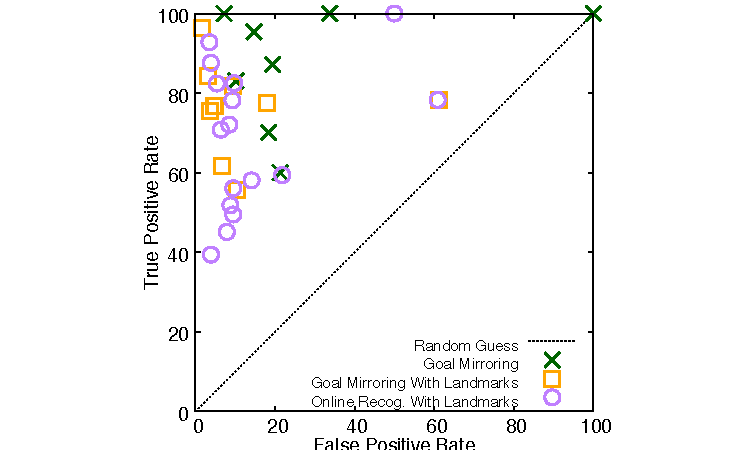
\includegraphics[width=.8\textwidth]{roc_space-online_approaches/rocspace-all_domains-online.pdf}
		\end{center}
	\end{frame}
	
	\begin{frame}[c]\frametitle{Efficiency Results}
		\begin{center}
			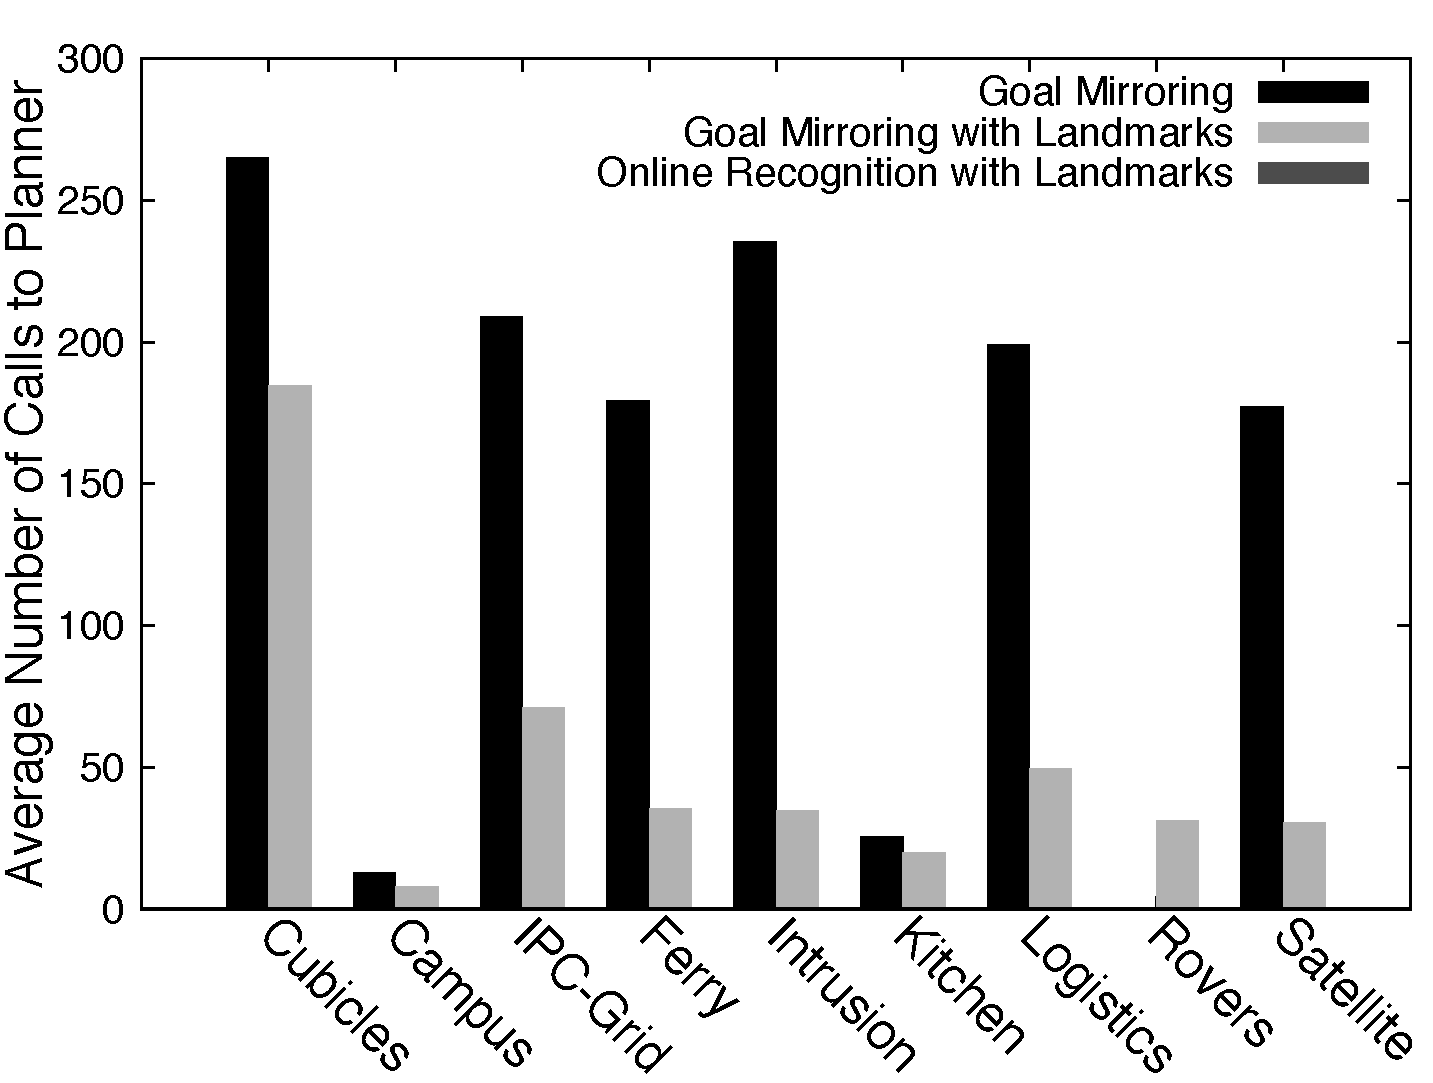
\includegraphics[width=.45\textwidth]{fig/histogram-number_of_calls_to_planner.pdf}
			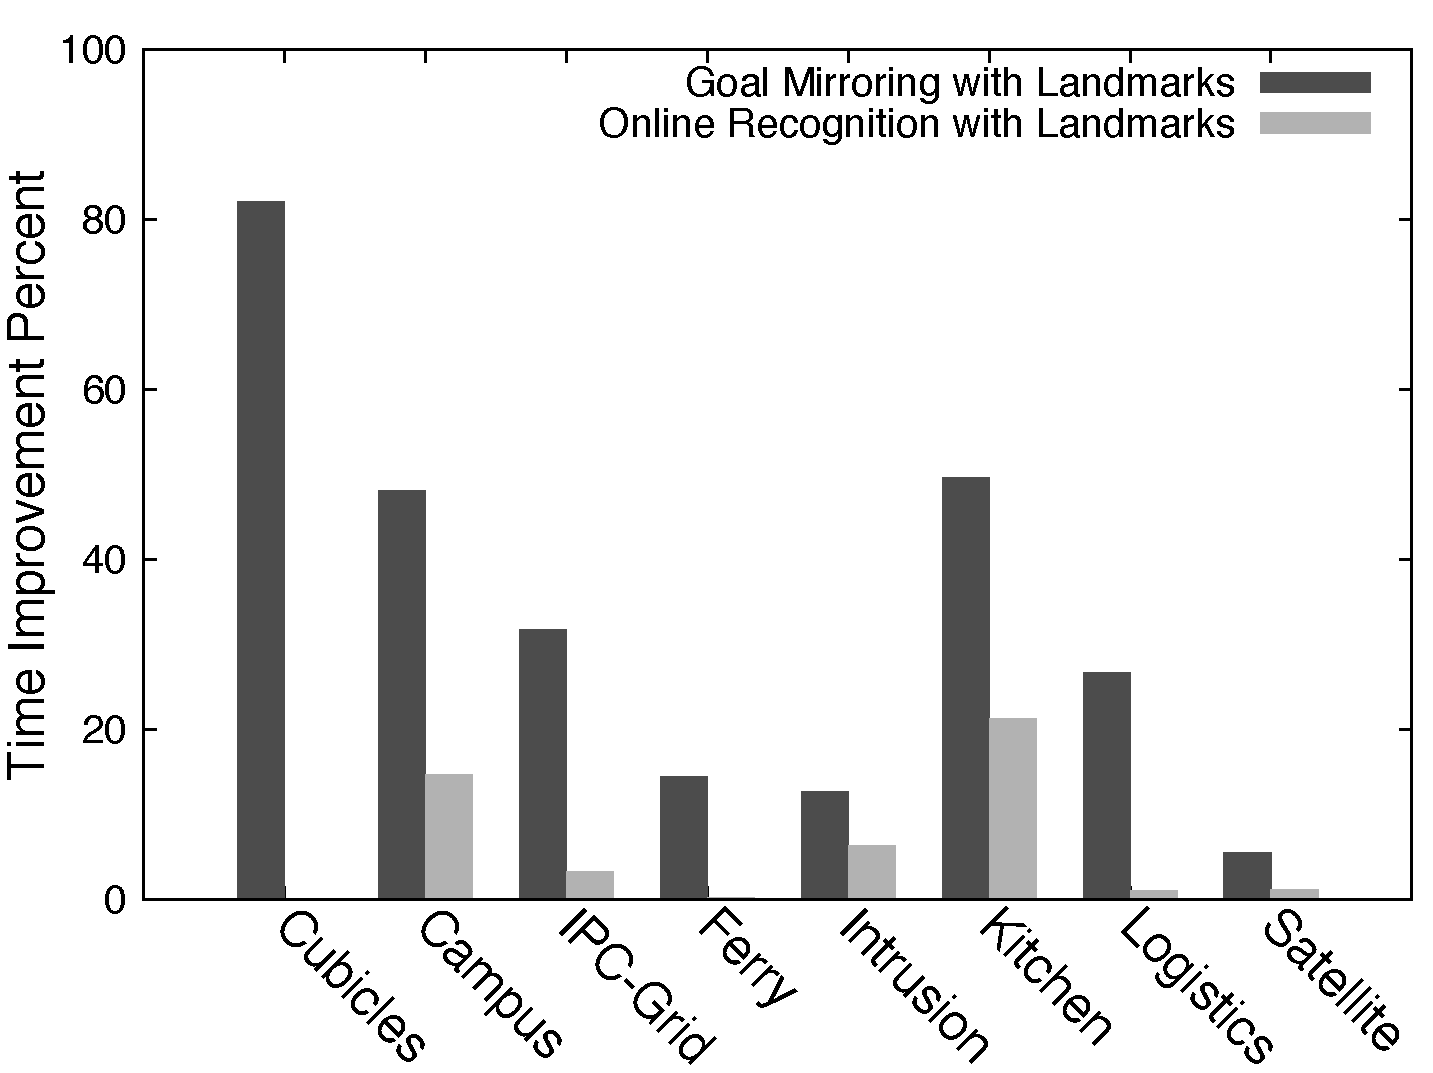
\includegraphics[width=.45\textwidth]{fig/histogram-time_improvement_percent.pdf}
		\end{center}
	\end{frame}
	
	\begin{frame}[c]\frametitle{Contributions and Limitations}
   	\begin{itemize}
   		\item \textbf{Contribution so far:}
			\begin{itemize}
				\item Extended de idea of landmarks for continuous domains; and
				\item Developed online algorithms able to recognize plans in\\ discrete and continuous domains;
				\item \textbf{Very} efficient in both discrete and continuous domains.
			\end{itemize}
		% \item We show that our heuristics are more accurate and much faster than Ramírez and Geffner's approach ({\footnotesize Plan Recognition as Planning. IJCAI, 2009}).
		\item \textbf{Limitations:}
			\begin{itemize}
				\item Naive notion of spatial landmarks;
				\item Much better performance on discrete domains.
			\end{itemize}
% 		\item \textbf{Future Work:}
% 			\begin{itemize}
% 				\item Use different landmark extraction algorithms;
% 				\item Use goal ordering techniques; 
% 				\item Derive a probabilistic interpretation for the landmarks; and
% 				\item Apply our landmark-based heuristics to continuous and temporal domains.
% 			\end{itemize}
	\end{itemize}
	\end{frame}

%---------------------------------------------------------------------------------

\if\masterclass1
\section{Goal Recognition in Incomplete Domains}

\subsection{Motivation and Background}

\begin{frame}[c]\frametitle{Motivation}
	\begin{itemize}
		\item So far, all goal recognition techniques assume that:
		\begin{itemize}
			\item domain knowledge is available;
			\item a domain engineer can build a \textbf{complete} and \textbf{correct} model of such domain knowledge 
			\item observations from sensor data agree with the model
		\end{itemize}
		\item However, most real world domains have two sources uncertainty:
		\begin{itemize}
			\item ambiguity in how actions performed by agents are realized; and
			\item ambiguity from how imperfect sensor data reports features of the world.
		\end{itemize}
		\item We aim to overcome both limitations by accepting \textbf{incomplete} domains
	\end{itemize}
\end{frame}

\begin{frame}[c]\frametitle{Overview}
	\begin{itemize}
		\item In this work, we develop a goal recognition approach that copes with \textbf{incomplete} planning \textbf{domain models}
		\item Our main contributions are:
		\begin{itemize}
			\item a new goal recognition formalization in incomplete domains
			\item the notion of \emph{potential landmarks} to deal with such incompleteness
			\item \emph{on-the-fly} landmark extraction techniques to deal with \emph{overlooked landmarks}
			\item an \textbf{efficient} goal recognition technique for incomplete domains
		\end{itemize}
		\item We evaluate the techniques empirically in an extensive new dataset that:
		\begin{itemize}
			\item includes hundreds of non-trivial problems
			\item includes various levels of domain model incompleteness
		\end{itemize}
	\end{itemize}
\end{frame}

\newcommand{\incp}[1]{\widetilde{\mathcal{#1}}}
\newcommand{\inc}[1]{\widetilde{#1}}
\newcommand{\pred}[1]{\texttt{\selectfont{#1}}}
\renewcommand{\lbrace}{[}
\renewcommand{\rbrace}{]}

\begin{frame}[c]\frametitle{Incomplete Planning Domain}
\begin{definition}[Incomplete Planning Domain]\label{def:planningIncompleteDomains}
An incomplete domain models is a tuple $\widetilde{\mathcal{D}} = \langle \mathcal{R}, \widetilde{\mathcal{O}} \rangle$, where:
\begin{itemize}
	\item $\mathcal{R}$ is the logic language
	\item $\widetilde{\mathcal{O}}$ is a set of incomplete operators $\inc{op} = \langle \mathit{pre}(\inc{op}), \widetilde{\mathit{pre}}(\inc{op}), \mathit{eff}^{+}(\inc{op}), \mathit{eff}^{-}(\inc{op}), \widetilde{\mathit{eff}}^{+}(\inc{op}), \widetilde{\mathit{eff}}^{-}(\inc{op}) \rangle$, where:
	\begin{itemize}
		\item $\mathit{pre}(\inc{op})$ and $\mathit{eff}(\inc{op})$ have the same semantics as in the STRIPS domain models;
		\item \textit{possible} preconditions $\widetilde{\mathit{pre}}(\inc{op}) \subseteq \mathcal{R}$; and
		\item \textit{possible} add and delete effects $\widetilde{\mathit{eff}}^{+}(\inc{op}) \subseteq \mathcal{R}$ and $\widetilde{\mathit{eff}}^{-}(\inc{op}) \subseteq \mathcal{R}$.
	\end{itemize}
\end{itemize}
\end{definition}
\begin{itemize}
	\item $\widetilde{\mathcal{D}}$ has a \textit{completion set} $\langle\langle \widetilde{\mathcal{D}} \rangle\rangle$ comprising all derivable domain models.
	\item $2^{\sum_{\inc{op} \in \widetilde{\mathcal{O}}}(|\widetilde{\mathit{pre}}(\inc{op})| + |\widetilde{\mathit{eff}}^{+}(\inc{op})| + |\widetilde{\mathit{eff}}^{-}(\inc{op})|)}$  such models
	\item single ground-truth model $\mathcal{D}^{*}$ that drives observed states. 
\end{itemize}
	% An incomplete planning problem derived from an incomplete domain $\incp{D}$ and a set of typed objects $Z$ is defined as $\incp{P} = \langle \mathcal{F}, \incp{\mathcal{A}}, \mathcal{I}, G \rangle$, where: $\mathcal{F}$ is the set of facts (instantiated predicates from $Z$), $\incp{\mathcal{A}}$ is the set of incomplete instantiated actions from $\inc{\mathcal{O}}$ with objects from $Z$, $\mathcal{I} \subseteq \mathcal{F}$ is the initial state, and $G \subseteq \mathcal{F}$ is the goal state.
\end{frame}

\begin{frame}[c]\frametitle{Incomplete domain example}
\begin{itemize}
	\item $\mathcal{F} = \lbrace p,q,r,g \rbrace$;
	\item $\incp{\mathcal{A}} = \lbrace \inc{a},\inc{b},\inc{c} \rbrace$, where:
	\begin{itemize}
		\item $\mathit{pre}(\inc{a}) = \lbrace p,q \rbrace, \widetilde{\mathit{pre}}(\inc{a}) = \lbrace r \rbrace, \widetilde{\mathit{eff}}^{+}(\inc{a}) = \lbrace r \rbrace, \widetilde{\mathit{eff}}^{-}(\inc{a}) = \lbrace p \rbrace$
		\item $\mathit{pre}(\inc{b}) = \lbrace p \rbrace, \mathit{eff}^{+}(\inc{b}) = \lbrace r \rbrace, \mathit{eff}^{-}(\inc{b}) = \lbrace p \rbrace, \widetilde{\mathit{eff}}^{-}(\inc{b}) = \lbrace q \rbrace$
		\item $\mathit{pre}(\inc{c}) = \lbrace r \rbrace, \widetilde{\mathit{pre}}(\inc{c}) = \lbrace q \rbrace, \mathit{eff}^{+}(\inc{c}) = \lbrace g \rbrace$
	\end{itemize}
	\item $\mathcal{I} = \lbrace p,q \rbrace$; and
	\item $G = \lbrace g \rbrace$.
\end{itemize}

Solution:
\begin{itemize}
	\item Here, $[\inc{a},\inc{b},\inc{c}]$ is a valid plan that achieves the goal stated $\lbrace g \rbrace$ from the initial state $\lbrace p,q \rbrace$.
	\item corresponds to  \textit{optimistic} state sequence:
	$s_{0} =  \lbrace p,q \rbrace, s_{1} = \lbrace p,q,r \rbrace, s_{2} = \lbrace q,r \rbrace, s_{3} = \lbrace q,r,g \rbrace$.
	\item This example has $2^{5}$ completion (2 possible preconditions and 3 possible effects).
\end{itemize}
\end{frame}

% \begin{frame}[c]\frametitle{Solving Problems in Incomplete Domains}
% 	\todo{Get material from Rao}
% \end{frame}

\begin{frame}[c]\frametitle{Goal Recognition in Incomplete Domain}
	\begin{definition}[\textbf{Goal Recognition Problem}]\label{def:GoalRecognitionIncompleteDomains}
	A goal recognition problem with an incomplete domain model is a quadruple $\incp{T} = \langle \incp{D}, Z, \mathcal{I}, \mathcal{G}, O \rangle$,
	where:
	\begin{itemize}
		\item $\incp{D} = \langle \mathcal{R}, \widetilde{\mathcal{O}} \rangle$ is an incomplete domain model;
		\item $Z$ is a set of typed objects in the environment, $\mathcal{F}$ is a set instantiated facts from $Z$, and $\incp{\mathcal{A}}$ is a set of instantiated incomplete actions from $\inc{\mathcal{O}}$ with objects from $Z$;
		\item $\mathcal{I} \in \mathcal{F}$ an initial state;
		\item $\mathcal{G}$ is a set of possible goals, including a hidden goal $G$; and
		\item $O = \langle o_1, o_2, ..., o_n\rangle$ is an observation sequence.
	\end{itemize}
	\end{definition}
	
	Each observation $o_i \in \incp{\mathcal{A}}$. $O$ corresponds to the sequence of actions (\idest, a plan) that achieves the correct hidden goal $G$ in a complete domain in $\langle\langle \widetilde{\mathcal{D}} \rangle\rangle$.
\end{frame}



% \begin{frame}[c]\frametitle{Problem Example}
%
% \end{frame}


\subsection{Landmarks in Incomplete Domains}

\begin{frame}[c]\frametitle{Optimistic RPG and Landmarks}
	\begin{center}
		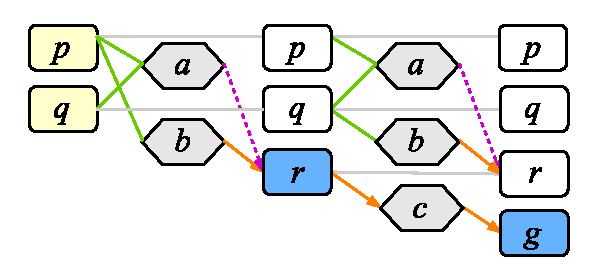
\includegraphics[width=.55\textwidth]{fig/ORPG-Example.pdf}
	\end{center}
	\begin{itemize}
		\item Previous approaches to landmark-based plan recognition extract landmarks using a \emph{Relaxed Planning Graph} (RPG)
		\item In order to cope with uncertainty, we build an \emph{optimistic} RPG
		\begin{itemize}
			\item ignores all \emph{possible} preconditions and delete effects \\ (definite and possible)
			\item includes all \emph{possible add} effects to the graph
		\end{itemize}
		\item Extracted landmarks are now either \emph{definite} of \emph{possible}
	\end{itemize}
\end{frame}

\begin{frame}[c]\frametitle{Definite and Possible Landmarks}
	\begin{center}
		\vspace{-2em}
		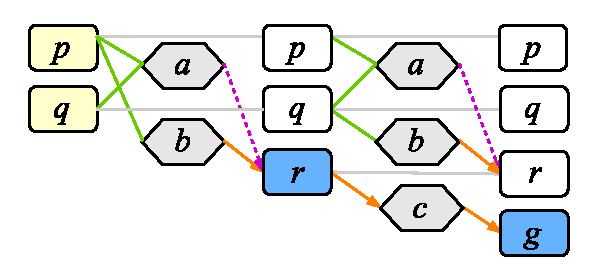
\includegraphics[width=.55\textwidth]{fig/ORPG-Example.pdf}
	\end{center}
	\vspace{-1.5em}
	\begin{definition}[\textbf{Definite Landmark}]\label{def:DefiniteLandmark}
	A \textit{definite} landmark $L_{Definite}$ is a fact (landmark) extracted from a known add effect ($\mathit{eff}^{+}(a)$) of an achiever $a$ (action) in the ORPG.
	\end{definition}
	\begin{definition}[\textbf{Possible Landmark}]\label{def:PossibleLandmark}
	A \textit{possible} landmark $L_{Possible}$ is a fact (landmark) extracted from a possible add effect ($\widetilde{\mathit{eff}}^{+}(a)$) of an achiever $a$ (action) in the ORPG.
	\end{definition}
	
\end{frame}

\newcommand{\set}[1]{\{#1\}}

\begin{frame}[c]\frametitle{Definite and Possible Landmarks}
	\begin{center}
		\vspace{-2em}
		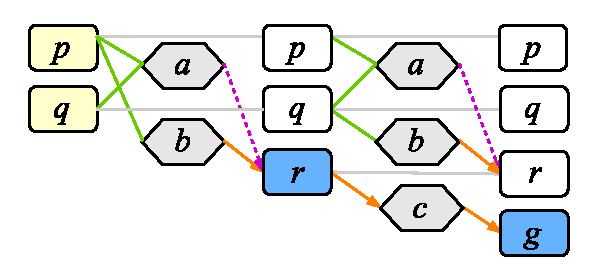
\includegraphics[width=.55\textwidth]{fig/ORPG-Example.pdf}
	\end{center}
	\vspace{-1.5em}
	\begin{itemize}
		\item Landmarks: $\set{p,q,r,g}$
		\begin{itemize}
			\item Definite Landmarks: $\set{r,g}$
			\item Possible Landmarks: $\set{p,q}$
		\end{itemize}
	\end{itemize}
\end{frame}

\subsection{Recognizing Goals in Incomplete Domains}

\begin{frame}[c]\frametitle{Computing Landmarks on the Fly}
\begin{itemize}
	\item Most \emph{efficient} landmark extraction algorithms (e.g. based on Relaxed Planning Graphs) are \emph{incomplete}\\
	Since extracting all landmarks is as difficult as planning itself
	\item Given the observations, we can focus landmark extraction to identify \emph{overlooked} landmarks 
	\begin{itemize}
		\item Rebuild the ORPG without an observation
		\item Check for satisfiability
	\end{itemize}
\end{itemize}
\end{frame}

\begin{frame}[c]\frametitle{Heuristic for Incomplete Domains}
	\begin{itemize}
		\item Combining these three types of landmarks, we define the $h_{\widetilde{GR}}(G)$ heuristic
		\begin{itemize}
			\item \textit{definite}  landmarks: $\mathcal{AL}_{G}$, $\mathcal{L}_{G}$;
			\item \textit{possible}  landmarks: $\mathcal{\widetilde{AL}}_{G}$, $\mathcal{\widetilde{L}}_{G}$; and
			\item \textit{overlooked} landmarks $\mathcal{ANL}_{G}$, $\mathcal{NL}_{G}$
		\end{itemize}
		\item $h_{\widetilde{GR}}(G)$ computes the ratio of achieved landmarks over computed ones
	\end{itemize}
$$h_{\widetilde{GR}}(G) = \left(\frac{\mathcal{AL}_{G} + \mathcal{\widetilde{AL}}_{G} + \mathcal{ANL}_{G}}{\mathcal{L}_{G} + \mathcal{\widetilde{L}}_{G} + \mathcal{NL}_{G}}\right)$$	
\end{frame}

\begin{frame}[c]\frametitle{Goal Recognition in Incomplete Domains}
	% \todo{Shrink this}
	    % \caption{{\footnotesize Recognize Goals in Incomplete Domain Models.}}
	    % \textbf{Input:} $\incp{T} = \langle \incp{D}, Z, \mathcal{I}, \mathcal{G}, O \rangle$, \textit{in which} $\incp{D}$ \textit{is an incomplete domain model}, $Z$ \textit{is a set of typed objects}, $\mathcal{I}$ \textit{is the initial state}, $\mathcal{G}$ \textit{is the set of candidate goals}, \textit{and} $O$ \textit{represents observations with incomplete action sequences}.
% 	    \\\textbf{Output:} \textit{Recognized goal(s).}
	    \label{alg:RecognizeIncompleteDomains}
	    \begin{algorithmic}[1]
			{\footnotesize
	        \Function{recognize}{$\incp{D}, Z, \mathcal{I}, \mathcal{G}, O$}
			\State $\mathcal{H}_{\mathcal{G}} \gets \langle \rangle$ \Comment{{\scriptsize \textit{Map goals to heuristic estimated values}.}}
	        \For{\textbf{each} goal $G$ in $\mathcal{G}$}
				\State $\mathcal{NL}_{G} \gets \langle \rangle$ \Comment{{\scriptsize \textit{Set of overlooked landmarks for G}.}}
				\State $\mathcal{L}_{G}, \mathcal{\widetilde{L}}_{G} \gets \textsc{extractLandmarks}(\incp{D}, Z, \mathcal{I}, G$) %\Comment{{\scriptsize \textit{Extracted definite and possible landmarks for G from $\mathcal{I}$}.}}\label{alg:RecognizeIncompleteDomains:ExtractLandmarks}
				\State $\mathcal{AL}_{G}, \mathcal{\widetilde{AL}}_{G}, \mathcal{ANL}_{G} \gets \langle \rangle$ \Comment{{\scriptsize \textit{Achieved landmarks}.}}
				\For{\textbf{each} observed action $o$ in $O$}
					\State $OF_{o} \gets$ all facts in $\mathit{pre}(o) \cup \mathit{eff}^{+}(o) \cup \widetilde{\mathit{eff}}^{+}(o)$ \Comment{{\scriptsize \textit{Observed facts in the incomplete model of action o}.}}\label{alg:RecognizeIncompleteDomains:UpdateState}
					\State $\mathcal{AL}_{G} \gets $ all landmarks $l$ in $\mathcal{L}_{G}$ s.t $l \in OF_{o}$ \label{alg:RecognizeIncompleteDomains:AchievedDefiniteLandmarks}
					\State $\mathcal{\widetilde{AL}}_{G} \gets $ all landmarks $\inc{l}$ in $\mathcal{AL}_{G}$ s.t $\inc{l} \in OF_{o}$ \label{alg:RecognizeIncompleteDomains:AchievedPossibleLandmarks}
					\For{\textbf{each} fact $f$ in $OF_{o}$ s.t $f \notin (\mathcal{L}_{G} \cup \mathcal{\widetilde{L}}_{G})$}
						\If{\textsc{isLandmark($f, \mathcal{I}, G$)}} \label{alg:RecognizeIncompleteDomains:OverlookedLandmarks}
							\State $\mathcal{NL}_{G} \gets \mathcal{NL}_{G} \cup f$ \label{alg:RecognizeIncompleteDomains:OverlookedLandmarksStore}
							\State $\mathcal{ANL}_{G} \gets \mathcal{ANL}_{G} \cup f$ \label{alg:RecognizeIncompleteDomains:AchievedOverlookedLandmarks}
						\EndIf
					\EndFor
				\EndFor
				\State $\mathcal{H}_{\mathcal{G}} := \mathcal{H}_{\mathcal{G}} \cup \langle G,\left(\frac{\mathcal{AL}_{G} + \mathcal{\widetilde{AL}}_{G} + \mathcal{ANL}_{G}}{\mathcal{L}_{G} + \mathcal{\widetilde{L}}_{G} + \mathcal{NL}_{G}}\right)\rangle$ \Comment{{\scriptsize Estimate value for G using the \textit{Use $h_{\widetilde{GR}}$ heuristic}.}} \label{alg:RecognizeIncompleteDomains:Heuristic}
			\EndFor
			\State \textbf{return} {all $G$ s.t $\langle G, v \rangle \in \mathcal{H}_{\mathcal{G}}$ and \newline \hspace*{\algorithmicindent}{\phantom{return }} $v \geq (\max_{v_i}{ \langle G',v_i \rangle \in \mathcal{H}_{\mathcal{G}}})$} \label{alg:RecognizeIncompleteDomains:Return}
	        \EndFunction
			}
	    \end{algorithmic}
\end{frame}

\begin{frame}[c]\frametitle{Algorithm Example}
	\todo{Fill this in with an example}
\end{frame}


\subsection{Results}

\begin{frame}[c]\frametitle{Experiments}
	\begin{itemize}
		\item Our evaluation uses a modified version of our IPC dataset
		\item We automatically generated incomplete versions of these domains:
		\begin{enumerate}
			\item randomly move a percentage of known preconditions and effects into possible lists of preconditions and effects; 
			\item randomly add possible preconditions from delete effects that are not preconditions of a corresponding operator; and 
			\item randomly add into possible lists \\(of preconditions, add effects, or delete effects) predicates whose parameters fit into the operator signatures.
		\end{enumerate}
		\item Evaluated accuracy and runtime
	\end{itemize}
\end{frame}

\begin{frame}[c]\frametitle{Results Low Incompleteness}
	\begin{columns}
		\begin{column}{0.45\textwidth}
			\centering
		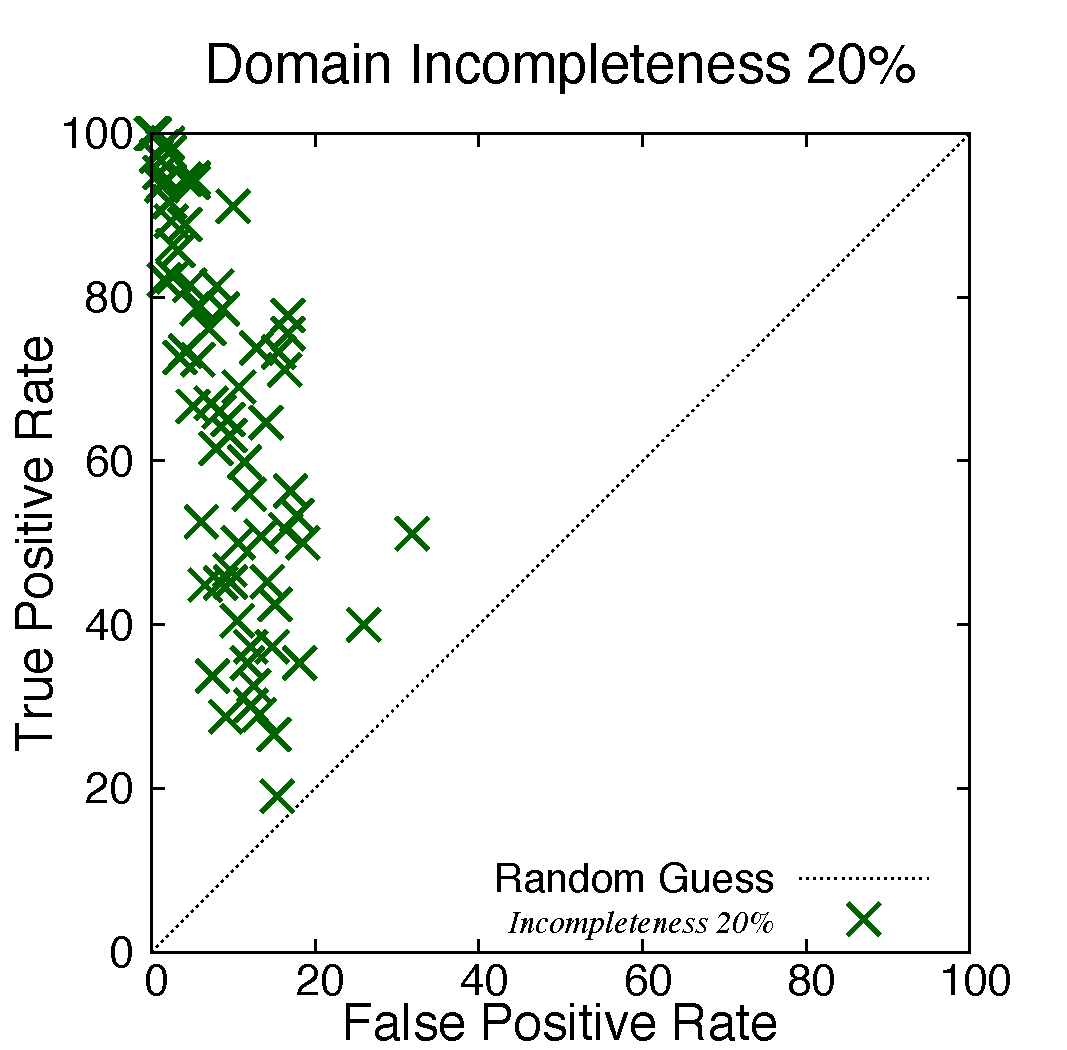
\includegraphics[width=.9\linewidth]{roc_space_incomplete/rocspace-domain_incompleteness-20.pdf}
		\end{column}
		\begin{column}{0.45\textwidth}
			\centering
		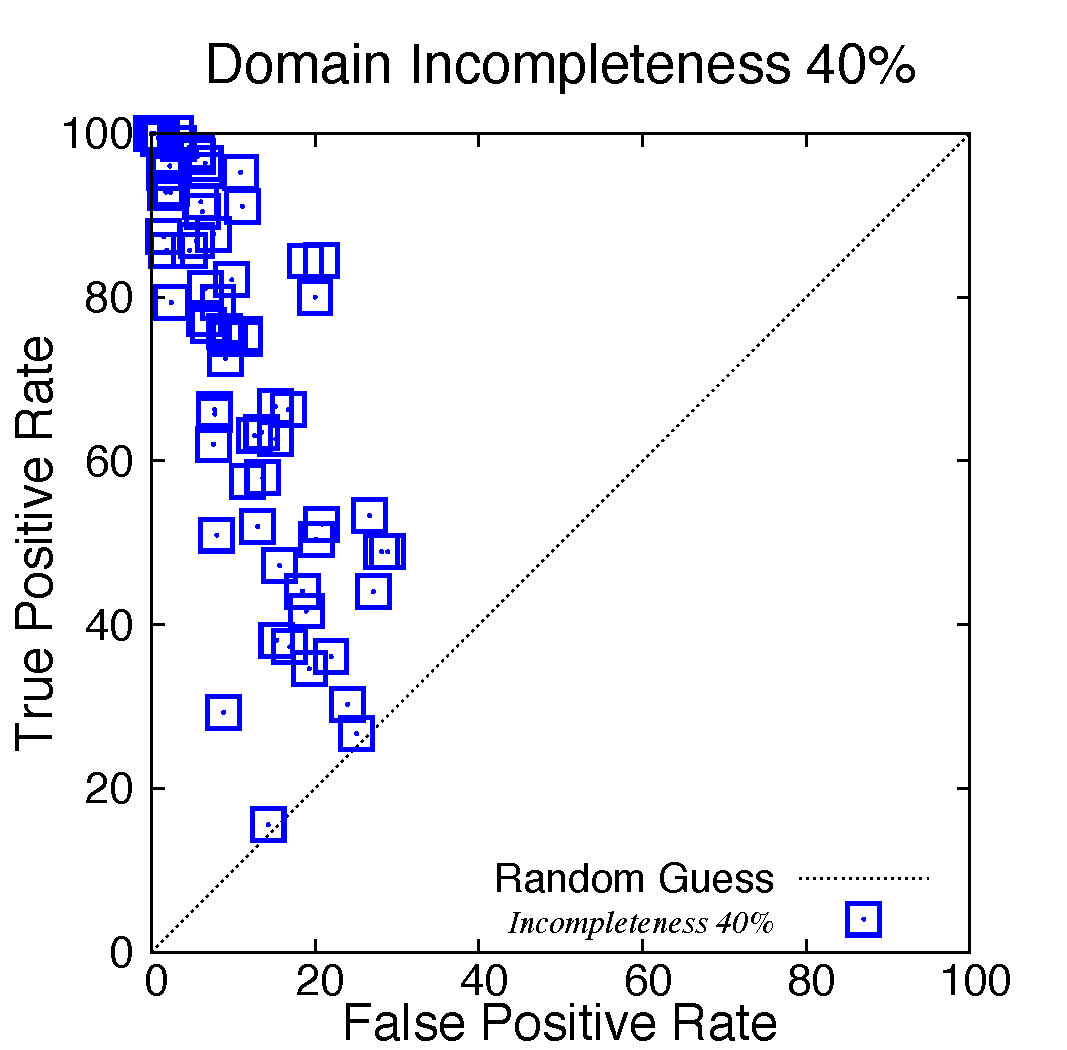
\includegraphics[width=.9\linewidth]{roc_space_incomplete/rocspace-domain_incompleteness-40.pdf}
		\end{column}
	\end{columns}
\end{frame}

\begin{frame}[c]\frametitle{Results High Incompleteness}
	\begin{columns}
		\begin{column}{0.45\textwidth}
			\centering
		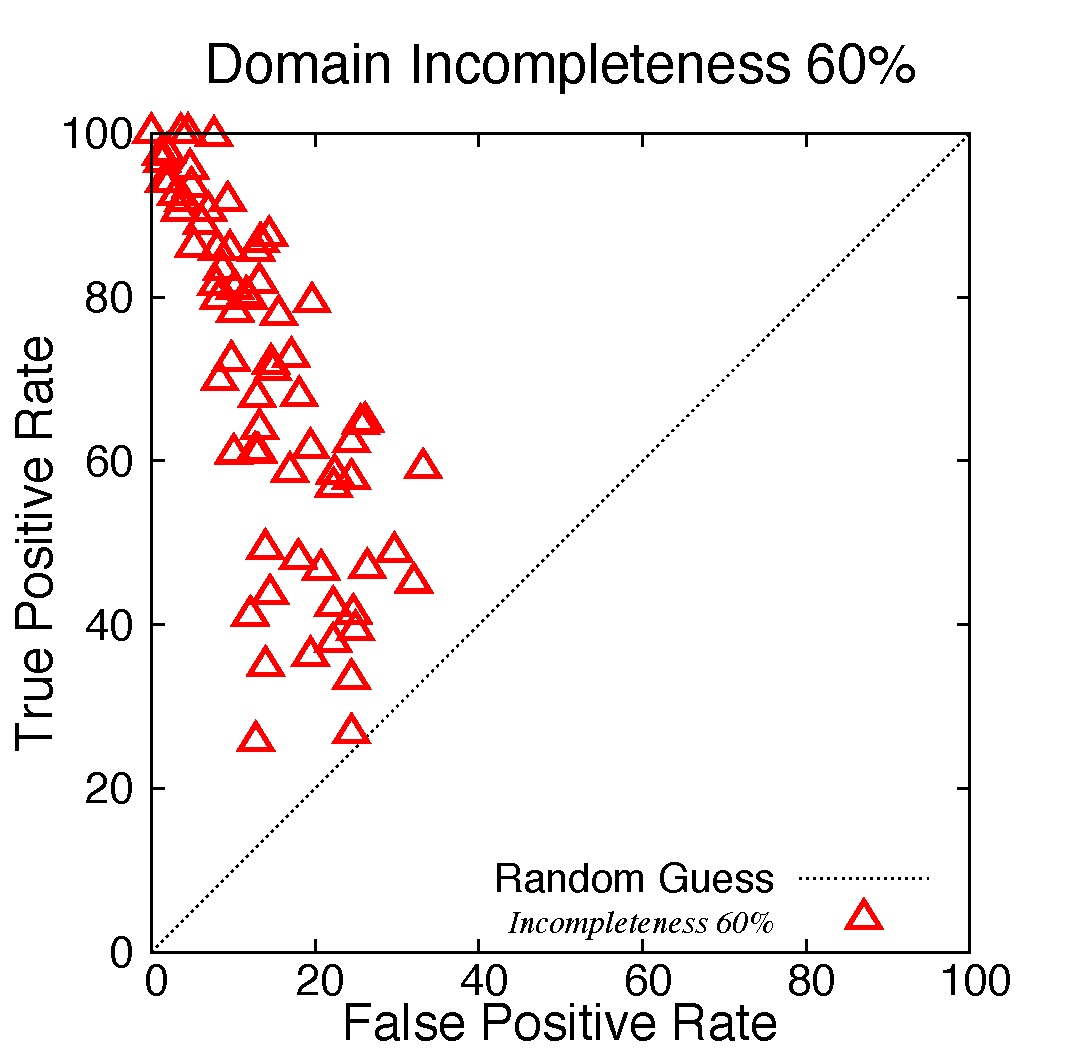
\includegraphics[width=.9\linewidth]{roc_space_incomplete/rocspace-domain_incompleteness-60.pdf}
		\end{column}
		\begin{column}{0.45\textwidth}
			\centering
		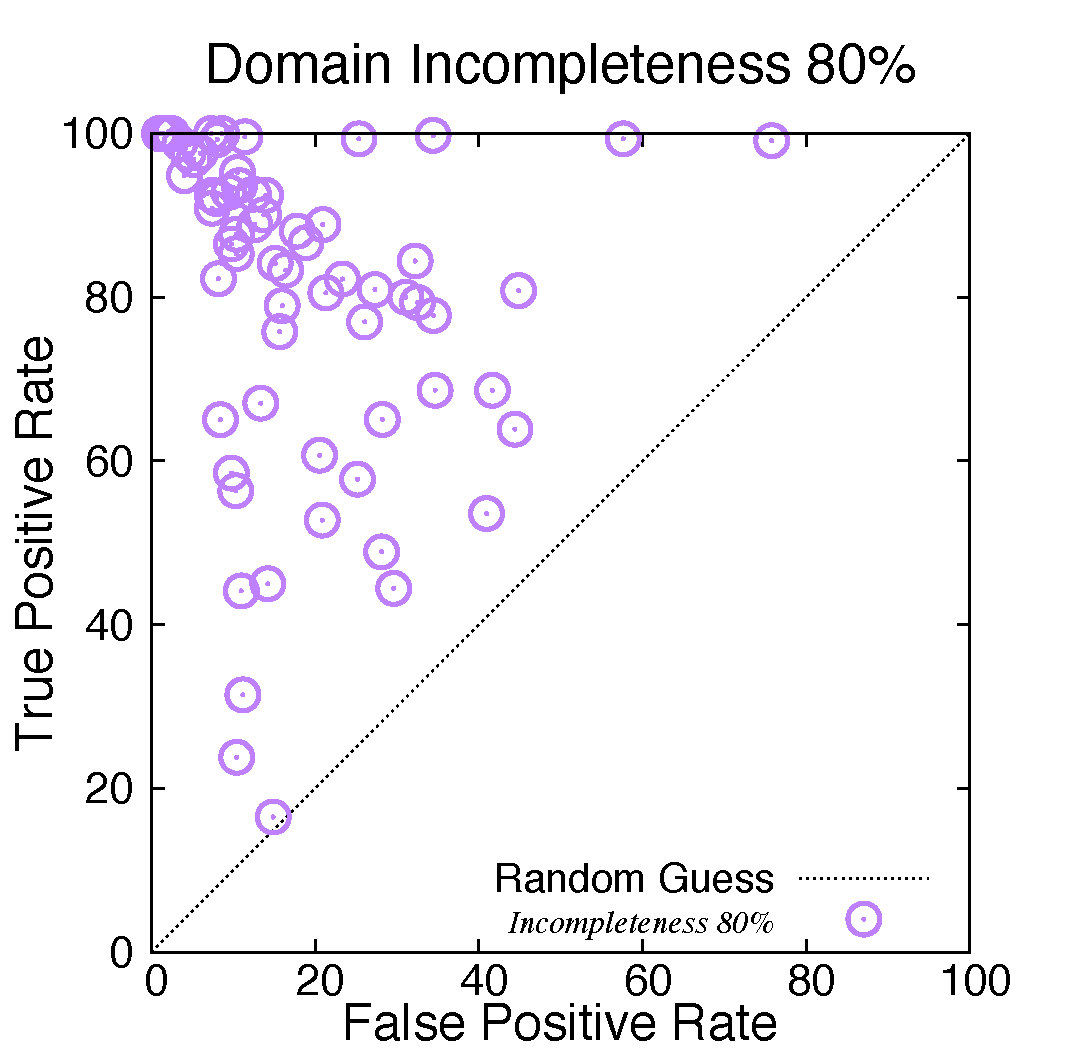
\includegraphics[width=.9\linewidth]{roc_space_incomplete/rocspace-domain_incompleteness-80.pdf}
		\end{column}
	\end{columns}
\end{frame}

\begin{frame}[c]\frametitle{Recognition Time}
	\todo{Add graph from Ramon}
\end{frame}

\fi

%---------------------------------------------------------------------------------

\section{Real World Applications}

\if\masterclass1
\subsection{Optimality Monitoring and Plan Abandonment}
\begin{frame}[c]\frametitle{Optimality Monitoring}
   	\begin{itemize}
   		\item Agents often \textbf{deviate} from the optimal plan for multiple reasons
		\begin{itemize}
			\item they have concurrent/multiple goals; or 
			\item they are not perfect optimizers;
		\end{itemize}
		\item We would like to be able to detect which actions in a plan do not advance (are non-optimal) towards a monitored goal;
		\item Our contribution is twofold:
			\begin{itemize}
				\item We formalize this problem using \textbf{planning domain definition}; and
				\item We combine two planning techniques to solve this problem: \textbf{landmarks} and \textbf{domain-independent heuristics}.
			\end{itemize}
		\item We evaluate our approach using several planning domains, and show that our approach yields \textbf{high accuracy} at \textbf{low computational cost}.
	\end{itemize}
\end{frame}

%---------------------------------------------------------------------------------

\begin{frame}[c]\frametitle{Background: Planning, Heuristics, and Landmarks}
	\vspace{-2mm}
	\begin{definition}[Planning]
		A planning instance is represented by a triple $\Pi = \langle \Xi, \mathcal{I}, G\rangle$, in which:
		\begin{itemize}
			\item $\Xi= \langle \Sigma, \mathcal{A}\rangle$ is the \textbf{domain definition}, and consists of a finite set of \textbf{facts} $\Sigma$ and a finite set of \textbf{actions} $\mathcal{A}$ (action costs $=$ 1);
			\item $\mathcal{I}$ and $G$ represent the \textbf{planning problem}, in which $\mathcal{I}$ $\subseteq$ $\Sigma$ is the \textbf{initial state}, and $G$ $\subseteq$ $\Sigma$ is the \textbf{goal state}.
		\end{itemize}
	\end{definition}
	\vspace{-3mm}
	\begin{itemize}
		\item \textbf{Heuristics} are used to estimate the cost to achieve a particular goal. In this work, we use \textbf{domain-independent heuristics};
	\end{itemize}
	\vspace{-3mm}
	\begin{definition}[Landmarks]
		Given a planning instance $\Pi = \langle \Xi, \mathcal{I}, G\rangle$, a \textbf{fact} (or \textbf{action}) $L$ is a landmark in $\Pi$ iff $L$ 	must be \textbf{satisfied} (or \textbf{executed}) at some point along all valid plans that achieve $G$ from $\mathcal{I}$.
	\end{definition}
\end{frame}

%---------------------------------------------------------------------------------

\begin{frame}[c]\frametitle{Plan Optimality Monitoring Problem}
	\begin{definition}[Plan Optimality Monitoring Problem]
		\begin{itemize}
   			\item Domain definition (Facts and Actions) $\Xi$ $=$ $\langle \Sigma, \mathcal{A} \rangle$;
   			\item Initial state \textbf{$\mathcal{I}$};
   			\item A monitored goal $G$; and
   			\item An observation sequence $O = \langle o_1, o_2, ..., o_n \rangle$, representing a full observable plan execution;
   		\end{itemize}			
	\end{definition}
    % FRM - I'm not sure I like the sentence below, I will try to rephrase it
	\begin{itemize}
		\item The solution to a plan optimality monitoring problem is the set of observations (\textbf{non-optimal actions}) that do not advance an optimal plan that the agent may be following.
	\end{itemize}
\end{frame}

\begin{frame}[c]\frametitle{Roboschool Example}
	\begin{columns}
		\begin{column}[t]{0.5\textwidth}
			{\color{red} Optimal Plan}\\
				\texttt{(walk roomb\_3 roomb\_4)}\\
				\texttt{(walk roomb\_4 rooma\_4)}\\
				\texttt{(pick p3 rooma\_4)}\\
				\texttt{(walk rooma\_4 roomb\_4)}\\
				\texttt{(walk roomb\_4 roomb\_3)}\\
				\texttt{(walk roomb\_3 roomb\_2)}\\
				\texttt{(walk roomb\_2 roomc\_2)}\\
				\texttt{(throw p3 roomc\_2 roomd\_2 b1)}\\
				\texttt{(pick p4 roomc\_2)}\\
				\texttt{(throw p4 roomc\_2 roomd\_2 b1)}\\
		\end{column}
			\begin{column}[t]{0.5\textwidth}
				{\color{red} Suboptimal Plan}\\
				\texttt{(walk roomb\_3 roomb\_4)}\\
				\texttt{(walk roomb\_4 rooma\_4)}\\
				\texttt{(pick p3 rooma\_4)}\\
				\texttt{(walk rooma\_4 roomb\_4)}\\
				\texttt{(walk roomb\_4 roomb\_3)}\\
				\texttt{(walk roomb\_3 roomb\_2)}\\
				\only<1>{\texttt{(walk roomb\_2 roomb\_1)}} 
				\only<2>{ {\color{red} \texttt{(walk roomb\_2 roomb\_1)} } }\\
				\only<1>{ \texttt{(walk roomb\_1 roomc\_1)} }
				\only<2>{{\color{red} \texttt{(walk roomb\_1 roomc\_1)} }}
				\\
				\texttt{(walk roomc\_1 roomc\_2)}\\
				\texttt{(throw p3 roomc\_2 roomd\_2 b1)}\\
				\texttt{(pick p4 roomc\_2)}\\
				\texttt{(throw p4 roomc\_2 roomd\_2 b1)}\\
		\end{column}
	\end{columns}
\end{frame}

%---------------------------------------------------------------------------------
\begin{frame}[c]\frametitle{Plan Optimality Monitoring Approach}
   	\begin{itemize}
   		\item Our approach \textbf{combines planning techniques}, \textit{i.e.}, landmarks and domain-independent heuristics.
		\item We use \textbf{landmarks} to obtain information about \textbf{what cannot be avoided} to achieve a monitored goal $G$; and
		\item We use \textbf{heuristics} to analyze possible \textbf{plan execution deviation}.
	\end{itemize}
\end{frame}
\begin{frame}[c]\frametitle{Analyzing Plan Execution Deviation}
   	\begin{itemize}
		\item If an observation $o_i$ results a state $s_i$, we consider a \textbf{deviation from a plan} to occur if $h(s_{i-1}) < h(s_i)$.
   	\end{itemize}
  	\begin{figure}[here]
		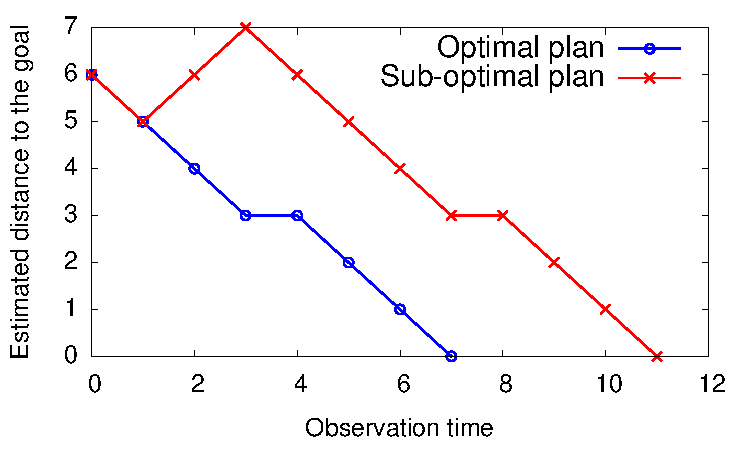
\includegraphics[width=0.85\linewidth]{fig/plan_execution-deviation.pdf}
	\end{figure} 
\end{frame}
%---------------------------------------------------------------------------------
\begin{frame}[c]\frametitle{Predicting Non-regressive Actions via Landmarks}
	\begin{itemize}
		\item To predict which actions could be executed in the next observation, we \textbf{analyze the closest landmarks by estimating the distance} (using $h_{max}$) from the current state to the extracted landmarks $\mathcal{L}$, namely:
			\begin{itemize}
				\item For every fact landmark $l \in \mathcal{L}$ in which the estimated \textbf{distance is 0},we select those actions $a \in \mathcal{A}$ such that $l \in \textit{pre}(a)$; and
				\item For every fact landmark $l \in \mathcal{L}$ in which the estimated \textbf{distance is 1}, we select those actions $a \in \mathcal{A}$ such that $pre(a) \in$ current state and $l \in \textit{eff}(a)^+$;
			\end{itemize}
		\item These predicted actions \textbf{may reduce the distance} to the \textbf{monitored goal} and \textbf{next landmarks}.
	\end{itemize}
\end{frame}

\begin{frame}[c]\frametitle{Finding Non-regressive actions}
	% \todo{Possibly avoid this slide}
    \begin{algorithmic}[1]
		\Require{$\Xi = \langle \Sigma, \mathcal{A} \rangle$ \textit{planning domain}, $\delta$ \textit{current state}, and $\mathcal{L}$ \textit{ordered fact landmarks}}
        \Function{NonRegressiveActions}{$\Xi$, $\delta$, $\mathcal{L}$}
        		\State $\eta_{PActions} \gets \langle$ $\rangle$
			\For{each fact landmark $l$ in $\mathcal{L}$} \label{alg:predictiNextActions:for}
				\State $Al \gets \langle \rangle$
            		\If{$h_{max}(l) = 0$} \Comment{\footnotesize $h_{max}(l)$ \textit{estimates} $l$ \textit{from} $\delta$.} \label{alg:predictiNextActions:h0}
            			\State $Al \gets$ all $a$ in $\mathcal{A}$ s.t. $l \in \textit{pre}(a)$ \label{alg:predictiNextActions:now}
				\ElsIf{$h_{max}$($l$) $=$ 1} \label{alg:predictiNextActions:h1}
					\State $Al \gets$ all $a \in \mathcal{A}$ s.t $\textit{pre}(a) \in \delta \land l \in \textit{eff}(a)^+$\label{alg:predictiNextActions:next}
				\EndIf
				\State $\eta_{PActions}$ := $\eta_{PActions}$ $\cup$ $Al$
            \EndFor
            	\State \textbf{return} $\eta_{PActions}$ \Comment{set of possible upcoming actions}
        \EndFunction
    \end{algorithmic}
\end{frame}

%---------------------------------------------------------------------------------
\begin{frame}[c]\frametitle{Detecting Sub-Optimal Steps}

	\begin{itemize}
		\item To detect sub-optimal steps (actions) in observation sequence $O$ for a monitored goal $G$, we combine the techniques we developed and filter with the following condition:
			\begin{itemize}
            	\item \textbf{An observed action $o \in O$ is considered sub-optimal if}: \\ $o$ $\notin$ set of predicted actions AND ($h(s_{i-1}) < h(s_i)$).
			\end{itemize}  
	\end{itemize}
\end{frame}


\begin{frame}[c]\frametitle{Detecting Sub-Optimal Steps (Monitor Plan Optimality)}
	% \vspace{-3mm}
%   	\begin{figure}[here]
% 		\includegraphics[width=0.73\linewidth]{algo-monitor_planoptimality.png}
% 	\end{figure}
    \begin{algorithmic}[1]
		\Require{$\Xi = \langle \Sigma, \mathcal{A}, \rangle$ \textit{planning domain}, $\mathcal{I}$ \textit{initial state}, $G$ \textit{monitored goal}, and $O$ \textit{observed actions}.}
		% \Ensure{$A_{SubOptimal}$ \textit{as sub-optimal actions}.}
        \Function{MonitorPlanOptimality}{$\Xi$,$\mathcal{I}$,$G$,$O$}
        		\State $A_{SubOptimal} \gets \langle\rangle$ \Comment{\footnotesize \textit{Non-contributing actions towards goal} $G$.}
        		\State $L \gets $ \textsc{ExtractLandmarks($\mathcal{I}$, $G$)}
			\State $\delta \gets \mathcal{I}$ \Comment{\footnotesize $\delta$ \textit{is the current state.}}
			\State $\eta_{PActions} \gets $ \textsc{NonRegressiveActions}($\Xi$, $\delta$, $L$)
			\State $D_{G} \gets$ \textsc{EstimateGoalDistance}($\delta$, $G$) \Comment{\footnotesize{\textit{Any domain-independent heuristic}}} 
        		\For{each observed action $o$ in $O$}
        			\State $\delta \gets \delta$.\textsc{Apply}($o$)
        			\State $D'_{G} \gets$ \textsc{EstimateGoalDistance}($\delta$, $G$)
        			\If{$o$ $\notin$ $\eta_{PActions}$ $\wedge$ $(D'_{G} > D_{G})$}\label{alg:monitor:estimatesuboptimalstep}
              		\State $A_{SubOptimal} \gets A_{SubOptimal} \cup o$
            		\EndIf
				\State $\eta_{PActions} \gets$ {\textsc{NonRegressiveActions}($\Xi$, $\delta$, $L$)}
        			\State $D_{G} \gets D'_{G}$
        		\EndFor
        		\State \textbf{return} $A_{SubOptimal}$
        \EndFunction
    \end{algorithmic}
\end{frame}

\begin{frame}[c]\frametitle{Example 1: Optimal Plan}
	\begin{columns}
		\begin{column}[t]{0.5\textwidth}
			{\Large Observations}\\
			\texttt{(walk roomb\_3 roomb\_4)}\\
			\texttt{(walk roomb\_4 rooma\_4)}\\
			\texttt{(pick p3 rooma\_4)}\\
			\texttt{(walk rooma\_4 roomb\_4)}\\
			\texttt{(walk roomb\_4 roomb\_3)}\\
			\texttt{(walk roomb\_3 roomb\_2)}\\
			\texttt{(walk roomb\_2 roomc\_2)}\\
			\texttt{(throw p3 roomc\_2 roomd\_2 b1)}\\
			\texttt{(pick p4 roomc\_2)}\\
			\texttt{(throw p4 roomc\_2 roomd\_2 b1)}\\
			
		\end{column}
		\begin{column}[t]{0.5\textwidth}
			{\Large $h_{\mathit{ff}}(o)$}
			\begin{tikzpicture}
				\begin{axis}[width=\textwidth,axis x line=bottom, axis y line=left, tick align=outside, xmin=0, ymin=0, xmax=12, ymax=10, xlabel=$o_{i}$, ylabel=$h_{\mathit{ff}}(o_{i})$]
					\addplot+[] coordinates{
											(0,8)
											(1,9)
											(2,9)
											(3,9)
											(4,8)
											(5,6)
											(6,4)
											(7,3)
											(8,2)
											(9,1)
											(10,0)
											};
					% \node[pin=0:{\small$\theta_1=0.5$}] at (axis cs:1,1) {};
% 					\addplot+[mark=none,smooth] (\x,{0.5*\x});
				\end{axis}
			\end{tikzpicture}
		\end{column}
	\end{columns}
\end{frame}

\begin{frame}[c]\frametitle{Example 2: Suboptimal Plan}
	\begin{columns}
		\begin{column}[t]{0.5\textwidth}
			{\Large Observations}\\
			\texttt{(walk roomb\_3 roomb\_4)}\\
			\texttt{(walk roomb\_4 rooma\_4)}\\
			\texttt{(pick p3 rooma\_4)}\\
			\texttt{(walk rooma\_4 roomb\_4)}\\
			\texttt{(walk roomb\_4 roomb\_3)}\\
			\texttt{(walk roomb\_3 roomb\_2)}\\
			\only<1>{\texttt{(walk roomb\_2 roomb\_1)}} 
			\only<2>{ {\color{red} \texttt{(walk roomb\_2 roomb\_1)} } }\\
			\only<1>{ \texttt{(walk roomb\_1 roomc\_1)} }
			\only<2>{{\color{red} \texttt{(walk roomb\_1 roomc\_1)} }}
			\\
			\texttt{(walk roomc\_1 roomc\_2)}\\
			\texttt{(throw p3 roomc\_2 roomd\_2 b1)}\\
			\texttt{(pick p4 roomc\_2)}\\
			\texttt{(throw p4 roomc\_2 roomd\_2 b1)}\\
			
			\vspace{1em}
			\only<2>{Suboptimal actions:\\ \texttt{(walk roomb\_2 roomb\_1)}}
		\end{column}
		\begin{column}[t]{0.5\textwidth}
			{\Large $h_{\mathit{ff}}(o)$}
			\begin{tikzpicture}
				\begin{axis}[width=\textwidth,axis x line=bottom, axis y line=left, tick align=outside, xmin=0, ymin=0, xmax=12, ymax=10, xlabel=$o_{i}$, ylabel=$h_{\mathit{ff}}(o_{i})$]
					\addplot+[] coordinates{
											(0,8)
											(1,9)
											(2,9)
											(3,9)
											(4,8)
											(5,6)
											(6,4)
											(7,5)
											(8,4)
											(9,3)
											(10,2)
											(11,1)
											(11,0)
											};
					\only<2>{
						\addplot+[only marks, color=red] coordinates{
											(7,5)
											};
					     \node[pin=90:{\tiny \texttt{(walk roomb\_2 roomb\_1)}}] at (axis cs:7,5) {};}
% 					\addplot+[mark=none,smooth] (\x,{0.5*\x});
				\end{axis}
			\end{tikzpicture}
			\only<2>{Step 7: \texttt{(walk roomb\_2 roomb\_1)}\\
			Expected Landmarks: None \\
			$h_{\mathit{ff}}(o_{7}) = 5$ 
			$h_{\mathit{ff}}(o_{6}) = 4$ 
			}
		\end{column}
	\end{columns}
\end{frame}
	
%---------------------------------------------------------------------------------
\begin{frame}[c]\frametitle{Experiments and Evaluation (1 of 2)}
   	\begin{itemize}
   		\item We evaluate our approach over 10 planning domains;
		\begin{itemize}
			\item Precision: percentage of correctly detected sub-optimal steps;
			\item Recall: percentage of true sub-optimal steps, actually detected. 
			% Here, a false negative is a sub-optimal action that is not detected by our approach. Recall provides the percentage of positive cases that our approach has detected.
		\end{itemize}
		\item We use 6 domain-independent heuristics: 
		\begin{itemize}
			\item $h_{adjsum}$, $h_{adjsum2}$, $h_{adjsum2M}$, $h_{combo}$, $h_{ff}$, and $h_{sum}$;
		\end{itemize}
		\item To extract landmarks and their ordering, we use an algorithm developed by Hoffman \emph{et al.} {\footnotesize (Ordered Landmarks in Planning. JAIR, 2004)};
		\item We manually generate the dataset from medium and large planning problems, containing both optimal and sub-optimal plan execution.
	\end{itemize}
\end{frame}

\begin{frame}[c]\frametitle{Experiments and Evaluation (2 of 2)}
	\begin{table}[]
		\scriptsize
		\centering
		\begin{tabular}{|c|c|c|c|cc|}
		\hline
		\textbf{Domain}             & $|O|$  & $|\mathcal{L}|$  & \textbf{Heuristic}          & \textbf{Time}        & \textbf{Precision / Recall / F1} \\ \hline
		\textsc{Blocks-World}  & 15.2 & 20.1 & $h_{adjsum2}$ / $h_{ff}$ 	& 0.19 / 0.21 & 100\% / 74.2\% / 85.2\%       \\ \hline
		\textsc{Driver-Log}    & 20.1 & 53.6 & $h_{adjsum2M}$            & 1.33        & 100\% / 100\% / 100\% 	  	  \\ \hline
		\textsc{Depots}        & 16.7 & 64.7 & $h_{adjsum2}$ / $h_{ff}$  & 1.22 / 1.43 & 81.2\% / 100\% / 89.6\%       \\ \hline
		\textsc{Easy-IPC-Grid} & 14.1 & 48.5 & $h_{adjsum2}$ / $h_{ff}$  & 0.77 / 0.86 & 100\% / 100\% / 100\%         \\ \hline
		\textsc{Ferry} 		  & 13.8 & 18.1 & $h_{adjsum}$ / $h_{sum}$  & 0.23 / 0.19 & 88.8\% / 78.5\% / 83.1\%        \\ \hline
		\textsc{Logistics}     & 20.8 & 24.0 & $h_{adjsum2}$ / $h_{ff}$  & 0.35 / 0.55 & 100\% / 91.3\% / 95.4\%       \\ \hline
		\textsc{Miconic}       & 18.1 & 19.4 & $h_{adjsum}$ / $h_{sum}$  & 0.29 / 0.21 & 100\% / 86.9\% / 93.1\%       \\ \hline
		\textsc{Satellite}     & 25.7 & 60.8 & $h_{adjsum2M}$        	& 9.58 		  & 88.8\% / 53.3\% / 66.6\%       \\ \hline
		\textsc{Sokoban}       & 24.0 & 76.5 & $h_{combo}$           	& 4.28		  & 90.9\% / 83.3\% / 86.9\%       \\ \hline
		\textsc{Zeno-Travel}   & 12.2 & 38.7 & $h_{adjsum2}$ / $h_{ff}$  & 0.86 / 0.99 & 100\% / 92.8\% / 96.2\%       \\ \hline
		\end{tabular}
        \caption{Plan Optimality Monitoring experimental (best) results.}
	\end{table}
\end{frame}	

%---------------------------------------------------------------------------------
\begin{frame}[c]\frametitle{Contributions and Limitations}
	% \todo{REDO THIS SLIDE}
   	\begin{itemize}
   		\item \textbf{Contribution:}
			\begin{itemize}
				\item Formalized plan optimality monitoring problem as planning;
				\item Developed an approach based on landmarks and heuristics;
				\item We show that our approach has high accuracy in almost all domains (besides \textsc{Satellite}).
			\end{itemize}
		\item \textbf{Limitations:}
			\begin{itemize}
				\item We do not yet deal with partial observability;
			\end{itemize}
		% \item \textbf{Future Work:}
% 			\begin{itemize}
%             	\item Evaluate our approach using more modern domain-independent heuristics;
% 				\item Try/use different landmark extraction algorithms; and
% 				\item Apply our approach to goal recognition (online and offline).
% 			\end{itemize}
	\end{itemize}
\end{frame}	
\fi
%---------------------------------------------------------------------------------	

% ================================
% = Plan recognition using video =
% ================================
\subsection{Plan Recognition using Video Data}
% \begin{frame}[c]\frametitle{Plan Recognition using Video Data}
% 	Get slides from Roger
% \end{frame}

\begin{frame}[c]\frametitle{Plan Recognition using Video Data}
	\begin{itemize}
   		\item \textbf{Plan recognition}
   		\begin{itemize}
				\item Task of recognizing the plan (i.e., the sequence of actions) the observed agent is following in order to achieve his intention (Sadri, 2012)
	    \end{itemize}
		\item \textbf{Activity recognition}
			\begin{itemize}
				\item The task of recognizing the independent set of actions that generates an interpretation to the movement that is being performed (Poppe,~2010)
				\item Such task is particularly challenging in the real physical world
			 \end{itemize}
		\item Much research effort focuses on activity and plan recognition as separate challenges;
		\item We develop a hybrid approach that comprises both activity and plan recognition;
		\item The approach infers, from a set of candidate plans, which plan a human subject is pursuing based exclusively on fixed-camera video.
	\end{itemize}
	\begin{flushright}
	{\tiny Poppe, R. A survey on vision-based human action recognition. \\Image and Vision Computing 28(6), pp. 976–990, 2010. \\
	       Sadri, Fariba. Intention Recognition in Agents for Ambient Intelligence: Logic-Based Approaches. \\ Ambient Intelligence and Smart Environments, pp. 197-236, 2012.
	}
	\end{flushright}
\end{frame}

\begin{frame}[c]\frametitle{A Hybrid Architecture for Activity and Plan Recognition}
   	\begin{itemize}
   		\item \textbf{Conceptually divided in two main parts}
   		\begin{itemize}
				\item CNN-based activity recognition (CNN)
                \item CNN-backed symbolic plan recognition (SBR)
	    \end{itemize}
	\end{itemize}
	\begin{center}
		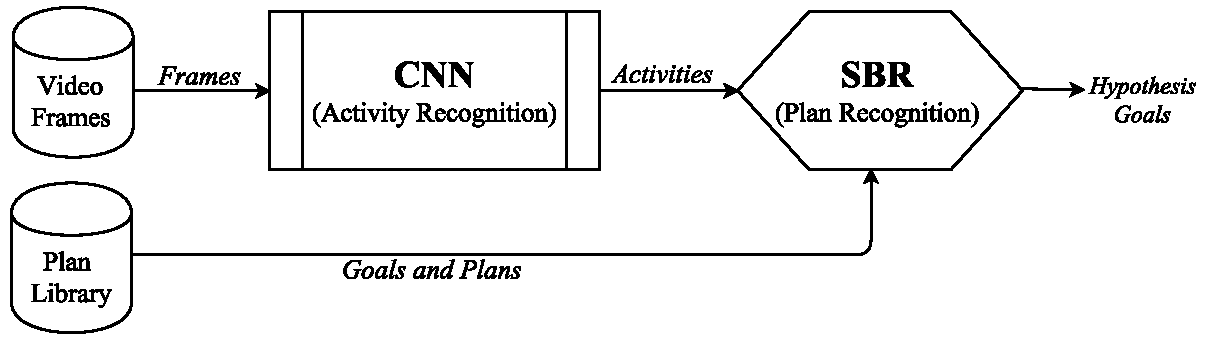
\includegraphics[width=0.8\linewidth]{fig/pipeline.pdf}
	\end{center}
\end{frame}

\if\masterclass1
\begin{frame}[c]\frametitle{CNN-based Activity Recognition}
   	\begin{itemize}
   		\item \textbf{Convolutional Neural Network}
   		\begin{itemize}
   		    \item Architecture: GoogLeNet
			\item 22-layer deep network based on the Inception module
            \item Input images: 224x224 (3 channels: RGB)
            \item Output classes: 9 (activities)
	    \end{itemize}
		
	\end{itemize}
\end{frame}

\begin{frame}{CNN-backed Symbolic Plan Recognition}
   	\begin{itemize}
   		\item \textbf{Symbolic Behavior Recognition (SBR)}
   		\begin{itemize}
				\item A plan recognition approach that takes as input a plan library and a sequence of observations
                \item Feature decision tree (FDT) maps observable features to plan-steps in a plan library
                \item SBR returns set of hypotheses plans such that each hypothesis represents a plan that achieves a top-level goal in a plan library
	    \end{itemize}
		\begin{center}
			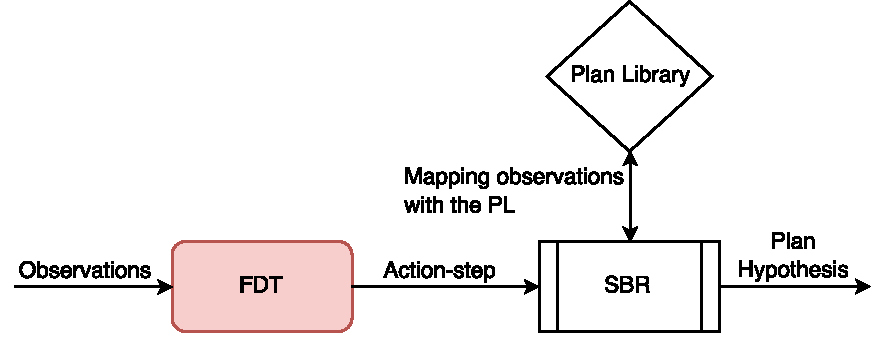
\includegraphics[width=0.7\linewidth]{fig/fdt.pdf}
		\end{center}
	\end{itemize}
\end{frame}

\begin{frame}[c]\frametitle{CNN-backed Symbolic Plan Recognition}
   	\begin{itemize}
   		\item \textbf{Our Symbolic Behavior Recognition}
   		\begin{itemize}
				\item We modify the SBR and replace the FDT with the CNN-backed Activity Recognition
                \item The CNN-backed Activity Recognition maps frames directly into nodes (activities) in the plan library used by SBR to compute sequential consistency of plan steps
	    \end{itemize}
		\begin{center}
			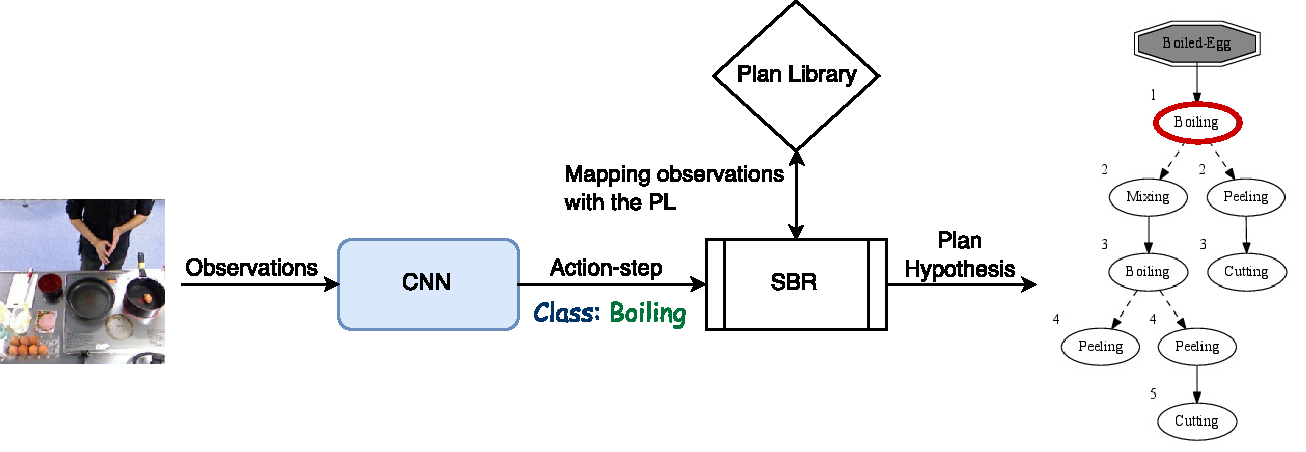
\includegraphics[width=0.9\linewidth]{fig/sbr.pdf}
		\end{center}
	\end{itemize}
\end{frame}
\fi

\begin{frame}{Experiments: Dataset}
   	\begin{itemize}
   		\item ICPR 2012 Kitchen Scene Context based Gesture Recognition dataset (KSCGR)%\footnote{http://www.murase.m.is.nagoya-u.ac.jp/KSCGR/}
	    \item \textbf{5 recipes for cooking eggs in Japan}
   		\begin{itemize}
				\item Ham and Eggs, Omelet, Scrambled-Egg, Boiled-Egg and Kinshi-Tamago
				\item Each recipe is performed by 7 subjects \\(5 in training set, 2 in testing set)
	    \end{itemize}
	    \item \textbf{9 cooking activities composes the dataset}
   		\begin{itemize}
				\item Breaking, mixing, baking, turning, cutting, boiling, seasoning, peeling, and none
	    \end{itemize}
		\begin{figure}[here]
			\centering
			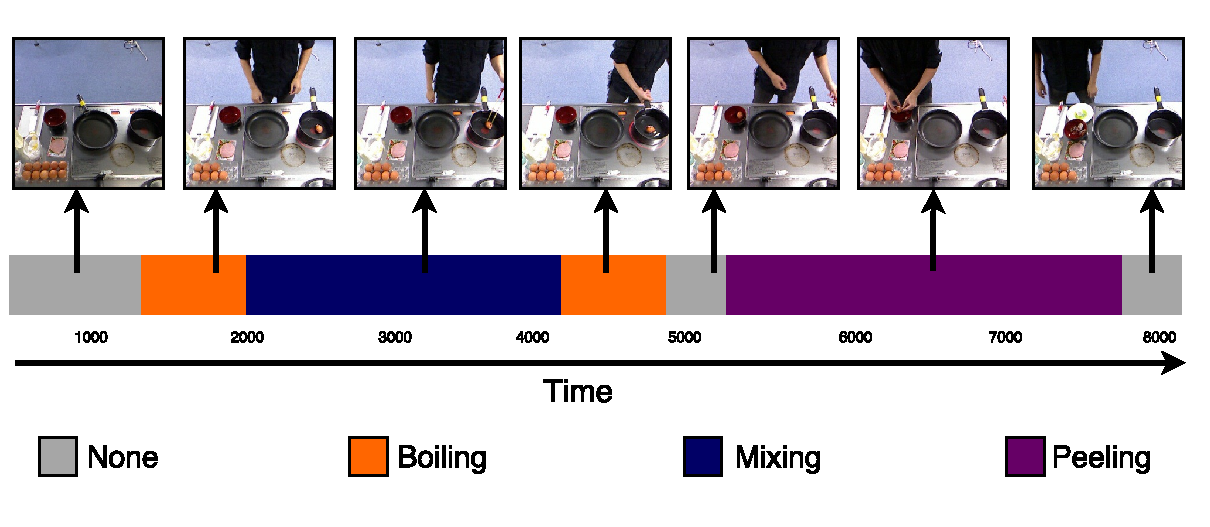
\includegraphics[width=0.7\linewidth]{fig/egg-dataset.pdf}
		\end{figure}
	\end{itemize}
\end{frame}

%---------------------------------------------------------------------------------
\if\masterclass1
\begin{frame}[c]\frametitle{Experiments: Plan Library Modeling}
   	\begin{itemize}
		\item We model a plan library containing knowledge of the agent's possible goals and plans based on the KSCGR dataset
		\item We consider that a sequence of cooking gestures is analogous to a sequence of a plan in the plan library
		\begin{figure}[here]
			\centering
			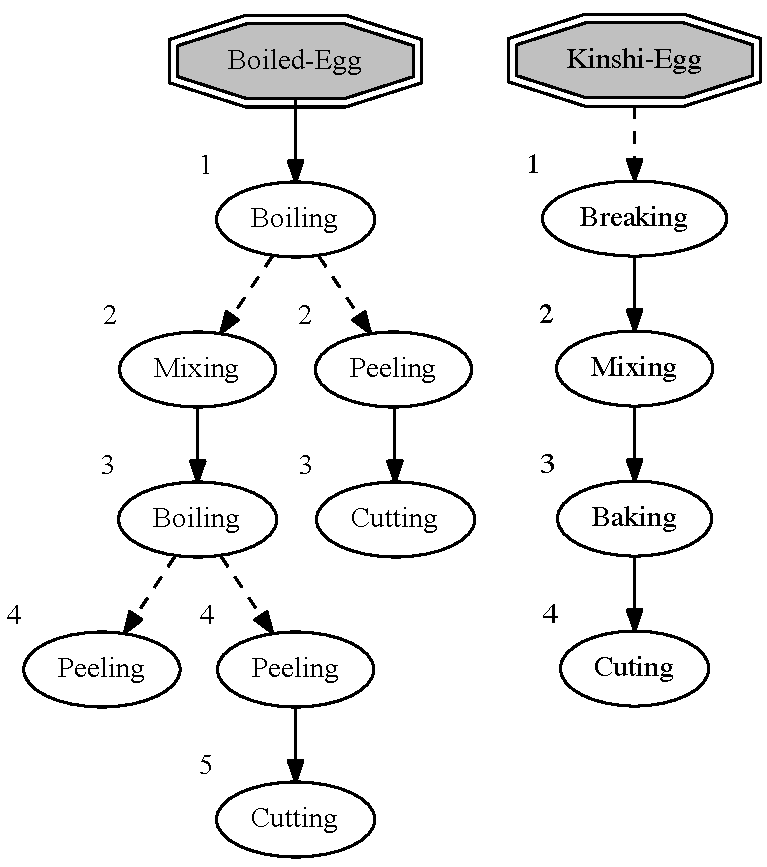
\includegraphics[width=0.4\linewidth]{fig/boiledegg-kinshiegg.pdf}
		\end{figure}
	\end{itemize}
\end{frame}

%---------------------------------------------------------------------------------
\iffalse
\begin{frame}[c]\frametitle{Experiments}
   	\begin{itemize}
   		\item \textbf{Convolutional Neural Network}: GoogLeNet
		\item Experiments separated into training, validation and test phases
		\item \textbf{Training phase}
   		\begin{itemize}
			\item Input images: 224x224
            \item Training stops after 30 epochs
	    \end{itemize}
	    \item \textbf{Validation phase}
   		\begin{itemize}
		    \item Select the model that achieves the highest accuracy
	    \end{itemize}
	    \item \textbf{Test phase}
   		\begin{itemize}
			\item CNN classifies each frame from input assigning to the image a probability score for each class
	    \end{itemize}
	\end{itemize}
\end{frame}
\fi 
%---------------------------------------------------------------------------------
\begin{frame}[c]\frametitle{Activity Recognition results}
	Precision, Recall, F-measure and Accuracy scores for each activity
	\begin{table}[tb!]
        \centering
        \footnotesize
        \begin{tabular}{l|cccc} 
            \hline\noalign{\smallskip}
            \textbf{Activity} & \textbf{Precision} & \textbf{Recall} & \textbf{F-measure} & \textbf{Accuracy} \\ 
            \noalign{\smallskip}\hline\hline\noalign{\smallskip}
            \textit{None}      &         0.65  & \textbf{0.97} &         0.78             &         0.64      \\ 
            \textit{Breaking}  &         0.44  &         0.41  &         0.42             &         0.27      \\
            \textit{Mixing}    &         0.67  &         0.34  &         0.45             &         0.29      \\
            \textit{Baking}    &         0.74  &         0.88  & \textbf{0.80}            & \textbf{0.67}     \\
            \textit{Turning}   &         0.77  &         0.38  &         0.51             &         0.34      \\
            \textit{Cutting}   &         0.87  &         0.63  &         0.73             &         0.58      \\
            \textit{Boiling}   &         0.61  &         0.34  &         0.43             &         0.28      \\
            \textit{Seasoning} & \textbf{0.89} &         0.37  &         0.52             &         0.35      \\
            \textit{Peeling}   &         0.72  &         0.10  &         0.18             &         0.09      \\
            \noalign{\smallskip}\hline
        \end{tabular}
    \end{table}
\end{frame}


%---------------------------------------------------------------------------------
\begin{frame}[c]\frametitle{Activity Recognition results}
	 Accuracy scores for each activity and the distribution of frames in KSCGR dataset
	
	\begin{minipage}{0.48\linewidth}
        \begin{table}[tb!]
            \centering
            \footnotesize
            \begin{tabular}{l|cc} 
                \hline\noalign{\smallskip}
                \textbf{Activity} & \textbf{Frames} & \textbf{Accuracy} \\ 
                \noalign{\smallskip}\hline\hline\noalign{\smallskip}
                \textit{None}      & \textbf{31\%}  & \textbf{0.64}     \\ 
                \textit{Breaking}  &          3\%   &         0.27      \\
                \textit{Mixing}    &         11\%   &         0.29      \\
                \textit{Baking}    & \textbf{25\%}  & \textbf{0.67}     \\
                \textit{Turning}   &          5\%   &         0.34      \\
                \textit{Cutting}   &          9\%   &         0.58      \\
                \textit{Boiling}   &          7\%   &         0.28      \\
                \textit{Seasoning} &          3\%   &         0.35      \\
                \textit{Peeling}   &          6\%   &         0.09      \\
                \noalign{\smallskip}\hline
            \end{tabular}
        \end{table}
    \end{minipage}
    \begin{minipage}{0.48\linewidth}
        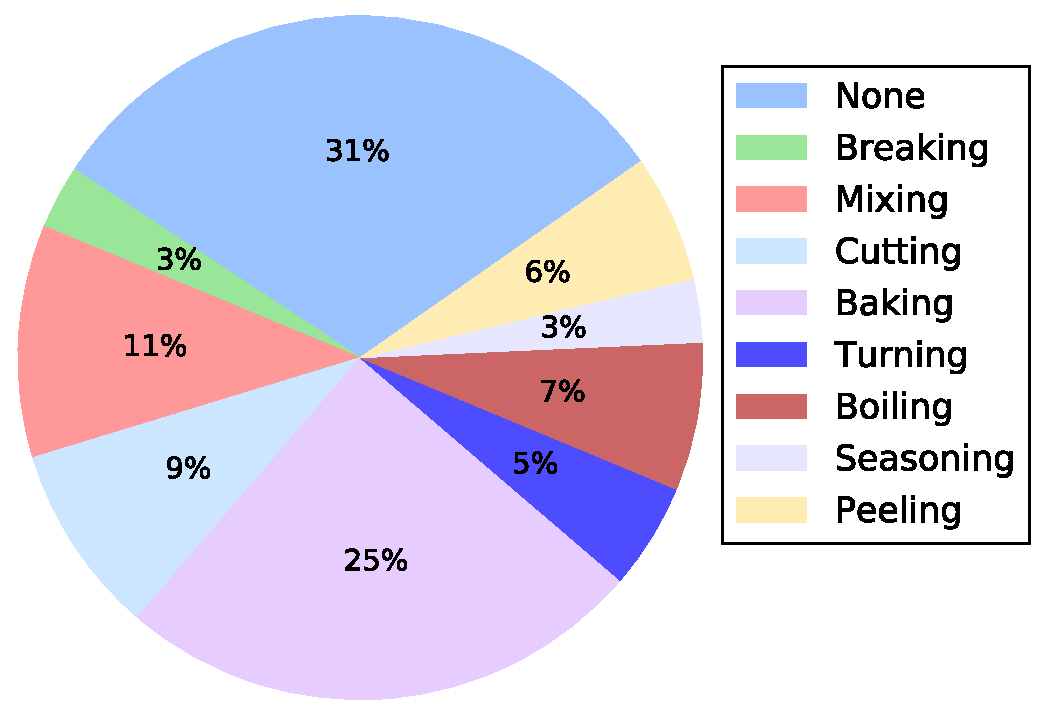
\includegraphics[width=\linewidth]{fig/perc.pdf}
    \end{minipage}
\end{frame}

%---------------------------------------------------------------------------------
% True labels in columns and predicted labels in lines, thus:
% The system should classify ``Breaking'' but instead some frames are classified as ``Peeling''
\begin{frame}[c]\frametitle{Activity Recognition results}
	Confusion matrix
	
	\begin{minipage}{0.48\linewidth}
        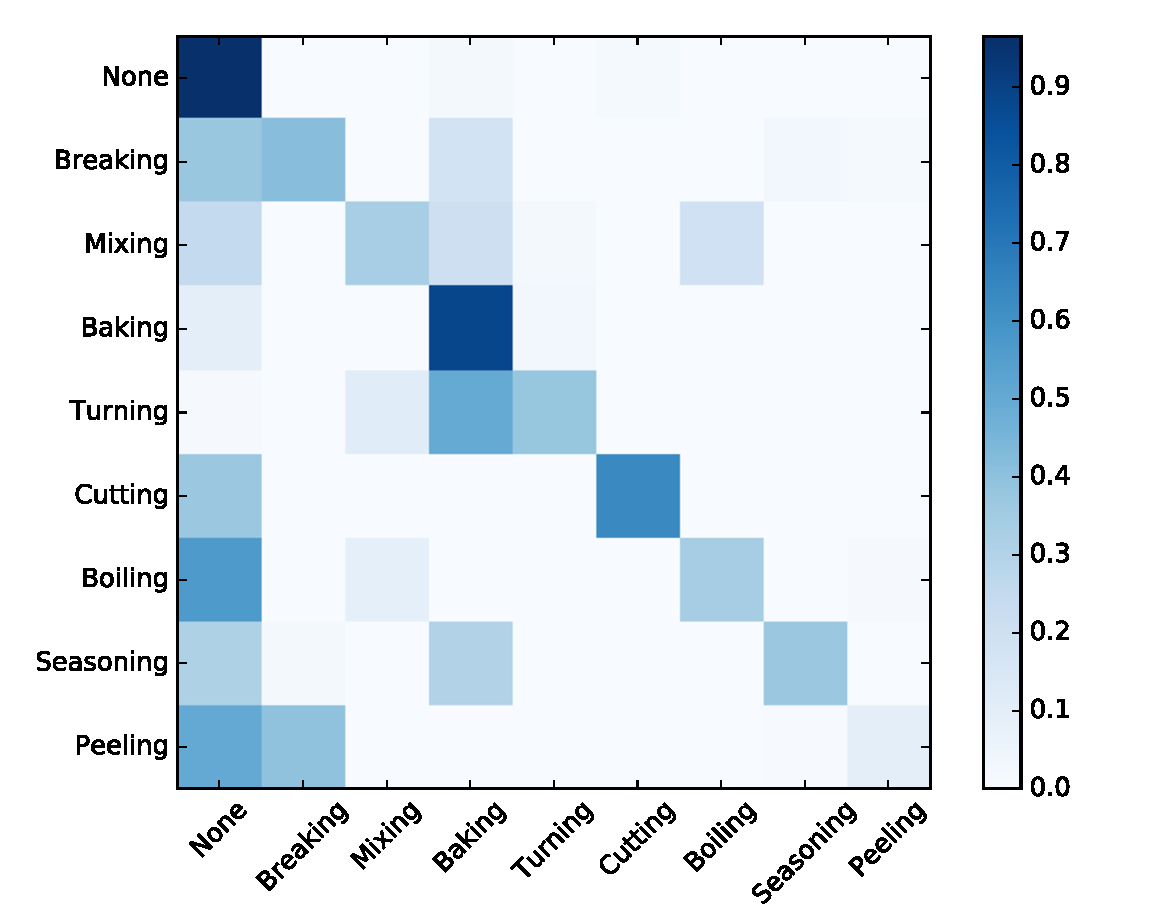
\includegraphics[width=\linewidth]{fig/egg-confusion_matrix.pdf}
    \end{minipage}
    \begin{minipage}{0.48\linewidth}
        \includegraphics[width=0.8\linewidth]{fig/egg-cooking-similar.pdf}
    \end{minipage}
    \begin{itemize}
		\item Close position in the scene
        \item Similar movements
    \end{itemize}
\end{frame}

%---------------------------------------------------------------------------------

\begin{frame}[c]\frametitle{Plan Recognition results}
   	\begin{itemize}
		\item We evaluate the whole pipeline using the number of hypotheses inferred by the plan recognizer
        \item \textbf{Score} weights correct predictions by the number of hypotheses
	\end{itemize}
	
	\begin{equation*}
        Score = \frac{c}{\#recipesFromSBR}
    \end{equation*}
    \begin{itemize}
		\item c: 1 if the correct recipe was inferred, 0 otherwise
        \item \#recipesFromSBR: Number of recipes yielded by the recognizer
    \end{itemize}
\end{frame}

%---------------------------------------------------------------------------------

\begin{frame}[c]\frametitle{Plan Recognition results}
    \begin{center}
        \scriptsize
        \begin{tabular}{l|llc} 
            \hline\noalign{\smallskip}
            \#                 & \textbf{True Recipe} & \textbf{Predicted Recipes} & \textbf{Score}\\ 
            \noalign{\smallskip}\hline\hline\noalign{\smallskip}
                              & Boiled-Egg   & Scramble-Egg, Omelette, Ham-Egg              & 0.00 \\ 
                              & Ham-Egg      & Scramble-Egg, Omelette                       & 0.00 \\
            10                & Kinshi-Egg   & Kinshi-Egg                                   & 1.00 \\
                              & Omelette     & Scramble-Egg, Omelette                       & 0.50 \\
                              & Scramble-Egg & Ham-Egg                                      & 0.00 \\
            \noalign{\smallskip}\hline\hline\noalign{\smallskip}
                              & Boiled-Egg   & Kinshi-Egg, Omelette, Ham-Egg                & 0.00 \\
                              & Ham-Egg      & Scramble-Egg                                 & 0.00 \\
            11                & Kinshi-Egg   & Scramble-Egg, Omelette, Ham-Egg              & 0.00 \\
                              & Omelette     & Kinshi-Egg, Scramble-Egg, Omelette, Ham-Egg  & 0.25 \\
                              & Scramble-Egg & Kinshi-Egg                                   & 0.00 \\
            \noalign{\smallskip}\hline\hline\noalign{\smallskip}
                                                        \multicolumn{3}{r}{\textbf{Average:}} & 0.18 \\
            \noalign{\smallskip}\hline
            \end{tabular}
    \end{center}
\end{frame}
\fi

%---------------------------------------------------------------------------------
\iffalse
\begin{frame}[c]\frametitle{Plan Recognition results}
   	\begin{itemize}
			\item Some activity sequences occur only in test set and not in training set
            \item Kinshi-Egg does not have any Turning activity in training set

    		{\scriptsize
    		\item[] \textbf{Dataset}: \#11 (testing set)
    		\item[] \textbf{Recipe}: Kinshi-Egg
    		\item[] \textbf{Activity sequence}: Breaking $\rightarrow$ Mixing $\rightarrow$ Baking $\rightarrow$ Turning $\rightarrow$ Baking $\rightarrow$ Cutting
    		}
	\end{itemize}
    \begin{itemize}
		\item Some sequences occur in more than one recipe in testing set
        \item[]

		{\scriptsize
		\item[] \textbf{Dataset}: \#11 (testing set)
		\item[] \textbf{Recipe}: Scrambled-Egg and Omelette
		\item[] \textbf{Activity sequence}: Breaking $\rightarrow$ Cutting $\rightarrow$ Seasoning $\rightarrow$ Mixing $\rightarrow$ Baking $\rightarrow$ Mixing $\rightarrow$ Baking
		}
    \end{itemize}
\end{frame}
\fi

\if\masterclass0
\begin{frame}[c]\frametitle{Summary of the Results}
	Conducted experiments on two levels:
	\begin{itemize}
		\item Activity Recognition
		\begin{itemize}
			\item Accuracy lower than 50\% (in 9-label classification) for infrequent activities
			\item Very good accuracy to identify ``no-action''
		\end{itemize}
		\item Overall Plan Recognition
		\begin{itemize}
			\item Low accuracy for overall plan recognition using plan-libraries
		\end{itemize}
	\end{itemize}
\end{frame}
\fi

%---------------------------------------------------------------------------------
\begin{frame}{Contributions and Future Work}
   	\begin{itemize}
   		\item We developed a hybrid architecture for activity and plan recognition
        \item Pipeline includes:
        \begin{itemize}
            \item A CNN for activity recognition that feeds directly into:
            \item a modified (SBR) approach that uses the CNN to index activities in the plan library
        \end{itemize}
        
        \item Approach limited by the plan library in the plan recognizer
        \item Next steps:
		\begin{itemize}
			\item Employ other deep learning architectures such as Long-Short Term Memory networks (LSTM) and 3D CNNs
	        \item Use a more flexible approach for plan recognition, such as PRAP
	        \item Explore object recognition to provide additional clues of the activity that is being performed 
		\end{itemize}
		\begin{center}
			Demo video: \url{https://youtu.be/BoiLjU1vg3E}
		\end{center}
    \end{itemize}
\end{frame}

%---------------------------------------------------------------------------------

%---------------------------------------------------------------------------------

% \begin{frame}[c]\frametitle{Motivation}
% 	\begin{itemize}
% 		\item Activity recognition:
% 		\begin{itemize}
% 			\item \emph{The task of recognizing the independent set of actions that generates an interpretation to the movement that is being performed} (Poppe,~2010)
% 			\item Such task is particularly challenging in the real physical world
% 		\end{itemize}
% 		\item Advances in hardware and greater availability of data have allowed deep learning algorithms
% 		\item Encouraged by the state-of-the-art results in object recognition, detection and semantic segmentation more and more applications are relying on deep neural architectures to perform video-based tasks
% 	\end{itemize}
% 	\begin{flushright}
% 		{\tiny Poppe, R. A survey on vision-based human action recognition. \\Image and Vision Computing 28(6), pp. 976–990, 2010.}
% 	\end{flushright}
% \end{frame}
%
%
% \begin{frame}[c]\frametitle{Contributions}
%    	\begin{itemize}
% 		\item We address the problem of recognizing human activities in an indoor environment with a single static camera
% 		\item Resulting approach aims at supporting people in cooking activities, recognizing their actions when cooking meals
% 		\item Our approach relies on a deep neural architecture that comprises multiple convolutional neural networks (CNNs) that are fused prior to performing the action classification
% 	\end{itemize}
% 	\begin{center}
% 		\includegraphics[width=0.6\linewidth]{fig/dataset_imgs.jpg}
% 	\end{center}
% \end{frame}
%
% \begin{frame}[c]\frametitle{Recognition Pipeline}
%    	\begin{itemize}
%    	    \item Our architecture has three main components:
%         \begin{itemize}
% 			\item Data pre-processing
% 			\item Convolutional Neural Networks (CNNs) for action recognition
% 			\item Fusion strategies for final classification
% 	    \end{itemize}
% 	\end{itemize}
% 	\begin{center}
% 		\includegraphics[width=0.6\linewidth]{fig/pipeline.pdf}
% 	\end{center}
% \end{frame}

%---------------------------------------------------------------------------------
\section{Summary and Future Directions}

\begin{frame}[c]\frametitle{Publications}
	\footnotesize
	\begin{itemize}
	\item[] FRAGA PEREIRA, Ramon; MENEGUZZI, Felipe. \textbf{Landmark-based Plan Recognition.} ECAI, 2016.
	\item[] PEREIRA, Ramon F.; OREN, Nir; and MENEGUZZI, Felipe. \textbf{Landmark-Based Heuristics for Goal Recognition}. AAAI, 2017.
	\item[] PEREIRA, Ramon F.; OREN, Nir; and MENEGUZZI, Felipe. \textbf{Monitoring Plan Optimality using Landmarks and Domain-Independent Heuristics}. PAIR Workshop@AAAI, 2017.
    \item[] GRANADA, Roger L.; PEREIRA, Ramon F.; MONTEIRO, Juarez; BARROS, Rodrigo; RUIZ, Duncan; and MENEGUZZI, Felipe. \textbf{Hybrid Activity and Plan Recognition for Video Streams}. PAIR Workshop@AAAI, 2017.
    \item[] PEREIRA, Ramon F.; OREN, Nir; and MENEGUZZI, Felipe. \textbf{Detecting Commitment Abandonment by Monitoring Plan Execution}. AAMAS, 2017.
    \item[] MONTEIRO, Juarez; GRANADA, Roger; BARROS, Rodrigo and MENEGUZZI, Felipe. \textbf{Deep Neural Networks for Kitchen Activity Recognition}. IJCNN, 2017.
    \item[] VERED, Mor; PEREIRA, Ramon F.; MAGNAGUAGNO, Maurício C.; KAMINKA, Gal; and MENEGUZZI, Felipe. \textbf{Online Goal Recognition Combining Landmarks and Planning}. GRW@IJCAI, 2017.
	\end{itemize}
\end{frame}

\begin{frame}[c]\frametitle{Summary}
	\begin{itemize}
		\item We progressively relaxed many assumptions about plan recognition:
		\begin{itemize}
			\item Domain knowledge
			\item Quality of observations
			\item Exclusively discrete domains
			\item Precise domain knowledge
		\end{itemize}
		\item We illustrated applications of these techniques:
		\begin{itemize}
			\item Real world video-data
			\item Multiagent systems
		\end{itemize}
	\end{itemize}
\end{frame}

\begin{frame}[c]\frametitle{Future Directions}
	\begin{itemize}
		\item Plan Recognition with Domain Theories
        \begin{itemize}
        	\item Use different landmark extraction algorithms;
% 			\item Use goal ordering techniques; 
% 			\item Derive a probabilistic interpretation for the landmarks; and
% 			\item Apply our landmark-based heuristics to continuous and temporal domains.
			\item Extend landmark-based heuristics to temporal and non-uniform-cost domains
            \item Experiment with more advanced notions of numeric landmarks \\(e.g. Scala et al.)
        \end{itemize}
        \item Applications of Plan Recognition
        \begin{itemize}
        	\item Use object recognition techniques (deep learning) to generate fact observations in video
            \item Couple the above with plan recognition in domain theories
            \item Do plan recognition in latent space
        \end{itemize}
	\end{itemize}
\end{frame}

\begin{frame}[c]\frametitle{Thanks and Acknowledgement}
	People involved in this research
	\begin{itemize}
		\item Ramon Fraga Pereira (PhD Student)
		\item Mor Vered (PhD Student, Bar Ilan University)
		\item Maurício Magnaguagno (PhD Student)
		\item Juarez Monteiro (MSc Student)
		\item Roger Granada (Postdoc)
		\item Gal Kaminka (Bar Ilan University) 
		\item Nir Oren (University of Aberdeen)
		\item Rodrigo Barros (PUCRS colleague) 
		\item Duncan Ruiz (PUCRS colleague) 
	\end{itemize}
	Institutions
	\begin{itemize}
		\item The Scottish Informatics and Computer Science Alliance (SICSA) \\ Distinguished Visiting Fellowship (DVE)
		\item Conselho Nacional de Desenvolvimento Científico e Tecnológico (CNPq) -- PQ Fellowship
	\end{itemize}
\end{frame}

% \if\masterclass1
% \begin{frame}[c]\frametitle{Master Class Plug}
% 	If this talk was interesting and you want to know more, please come to:\\[2em]
% 	\begin{center}
% 		{\Large
% 		Plan Recognition Master Class \\[2em] University of Aberdeen -- 16th October 2017
% 		}
% 	\end{center}
% 	We will cover:
% 	\begin{itemize}
% 		\item Detailed algorithms
% 		\item Worked out examples
% 		\item Plan recognition with incomplete \textbf{domains}
% 		\item Much more
% 	\end{itemize}
% \end{frame}
%
% \fi

% \begin{frame}[c]\frametitle{Research Plug}
% 	If this class was interesting and you want to do research, consider a PhD:\\[2em]
% 	\begin{center}
% 		{\Large
% 		Plan Recognition Master Class \\[2em] University of Aberdeen -- 16th October 2017
% 		}
% 	\end{center}
% 	We will cover:
% 	\begin{itemize}
% 		\item Detailed algorithms
% 		\item Worked out examples
% 		\item Plan recognition with incomplete \textbf{domains}
% 		\item Much more
% 	\end{itemize}
% \end{frame}



	{
	\setbeamercolor{background canvas}{bg=lightgray}
    \begin{frame}{}
    		\centering
    		Thank you!
			\\
    \end{frame}
    }

%---------------------------------------------------------------------------------

\end{document}